%\documentclass[11pt]{article}
%\usepackage[margin=1in]{geometry}
%\usepackage[utf8]{inputenc}
%\usepackage{amsmath}
%\usepackage{xspace}
%\usepackage{graphicx}
%\usepackage{subfig}
%\usepackage{hyperref}
%\usepackage{lineno}
%\usepackage{stackengine}
%\usepackage{tabularx}
%\usepackage{rotating}
%\usepackage{braket}
%\usepackage{placeins}
%\usepackage{caption}
%\usepackage{float}
%\usepackage{subcaption}
%\usepackage{amssymb}
%\usepackage{authblk}

\documentclass{article}
\usepackage[utf8]{inputenc}
\usepackage{geometry}
\usepackage{lineno}
\usepackage{amsmath}
\usepackage{graphicx}
\usepackage{hyperref}
\usepackage{float}
\usepackage{tabularx}
\usepackage{rotating}
\usepackage{braket}
\usepackage{placeins}
\usepackage{caption}
\usepackage{float}
\usepackage{subcaption}
\usepackage{amssymb}
\usepackage{authblk}

%usepackage{subcaption}

\geometry{a4paper, margin=1in}



\begin{document}

\title{Detector Acceptance Calculation for Drell-Yan Process}
\author[1]{Chatura Kuruppu} 
\affil[1]{New Mexico State University, Las Cruces, NM 88003}
\date{\today}
\maketitle

\section{Introduction}

In experimental particle physics, detector acceptance is a crucial correction factor that quantifies the probability of a physics event being successfully detected and reconstructed by the experimental apparatus. Due to geometrical constraints, detector inefficiencies, and the kinematic requirements of event reconstruction algorithms, not all events produced in a collision are recorded. The acceptance, $A$, is therefore defined as the ratio of the number of events that are detected and pass all selection criteria ($N_{acc}$) to the total number of events generated within a specific kinematic phase space ($N_{gen}$).

\begin{equation}
\text{Acceptance (A)} = \frac{N_{acc}}{N_{gen}}
\label{eq:acceptance}
\end{equation}

This document outlines the step-by-step procedure for calculating the detector acceptance for the Drell-Yan process using Monte Carlo (MC) simulations. The acceptance is evaluated as a function of the dimuon invariant mass and Feynman-x ($x_F$) for both Liquid Hydrogen (LH2) and Liquid Deuterium (LD2) targets. The calculation is based on the analysis performed by the ROOT C++ script \texttt{run\_all\_plots.C}.

\section{Monte Carlo Files Used}

The calculation relies on pre-generated Monte Carlo simulation files. For each target, two distinct sets of data are used:

\begin{itemize}
    \item \textbf{Thrown Files:} These files contain the generated four-vector information for Drell-Yan events, simulated over a $4\pi$ solid angle. They represent the theoretical population of events ($N_{gen}$) before any detector effects are considered.
    \begin{itemize}
        \item \texttt{mc\_drellyan\_LH2\_M027\_S001\_4pi\_pTxFweight\_v2.root}
        \item \texttt{mc\_drellyan\_LD2\_M027\_S001\_4pi\_pTxFweight\_v2.root}
    \end{itemize}
    \item \textbf{Accepted Files:} These files contain events from the thrown sample that have been processed through a full detector simulation (e.g., Geant4) and reconstructed using the same algorithms applied to real experimental data. These events represent the detected population ($N_{acc}$).
    \begin{itemize}
        \item \texttt{mc\_drellyan\_LH2\_M027\_S001\_clean\_occ\_pTxFweight\_v2.root}
        \item \texttt{mc\_drellyan\_LD2\_M027\_S001\_clean\_occ\_pTxFweight\_v2.root}
    \end{itemize}
\end{itemize}
Each event in these files includes a \texttt{ReWeight} factor, which is used to adjust the MC simulation to better match the transverse momentum ($p_T$) distribution observed in experimental data. All calculated histograms are weighted by this factor.

\section{Event Selection}
To ensure a valid comparison, specific event selection criteria (cuts) are applied to both the thrown and accepted datasets.

\begin{itemize}
    \item \textbf{Thrown Sample Cut (\texttt{MCcut}):} A minimal cut is applied to the generated events to define the kinematic phase space of interest. In the provided script, this is set to \texttt{"1"}, indicating all generated events are considered.

    \item \textbf{Accepted Sample Cut (\texttt{allCut}):} A comprehensive set of cuts is applied to the reconstructed data. These cuts are designed to select high-quality dimuon events and mimic the selection criteria used in the final physics analysis. They are defined in external files (\texttt{chuckcuts.h}, \texttt{otherCuts.c}) and combined into a single \texttt{TCut} object.
\end{itemize}

\section{Kinematic Binning for Acceptance Study}
The acceptance is studied differentially across the invariant mass and $x_F$ variables. The binning schemes are defined in the header file \texttt{abs\_cs.h}.

\subsection{Feynman-x ($x_F$) Bins}
The analysis is performed in 16 discrete bins of $x_F$. The bin edges are defined as:
\begin{verbatim}
xFEdge[] = {0, 0.05, 0.1, 0.15, 0.2, 0.25, 0.3, 0.35,
            0.4, 0.45, 0.5, 0.55, 0.6, 0.65, 0.7, 0.75, 0.8};
\end{verbatim}

\subsection{Mass Bins}
Within each $x_F$ bin, the acceptance is calculated as a function of the dimuon invariant mass. The histograms are created with 10 mass bins defined by the following edges (in GeV/$c^2$):
\begin{verbatim}
massEdge[] = {4.5, 4.8, 5.1, 5.4, 5.7, 6, 6.3, 6.6,
              6.9, 7.5, 8.7};
\end{verbatim}

\section{Acceptance Plots for each $x_F$ Bin}
The following subsections show the resulting acceptance plots as a function of mass for each of the 16 $x_F$ bins. Each figure is arranged in a 2x2 grid displaying four plots:
\begin{itemize}
    \item \textbf{Top Left:} The detector acceptance for the LH2 target.
    \item \textbf{Top Right:} The detector acceptance for the LD2 target.
    \item \textbf{Bottom Left:} The combined average acceptance for both targets.
    \item \textbf{Bottom Right:} The ratio of the LH2 acceptance to the LD2 acceptance, used to check for target-dependent effects.
\end{itemize}

\begin{figure}[H]
    \centering
    \begin{subfigure}[b]{0.48\textwidth}
       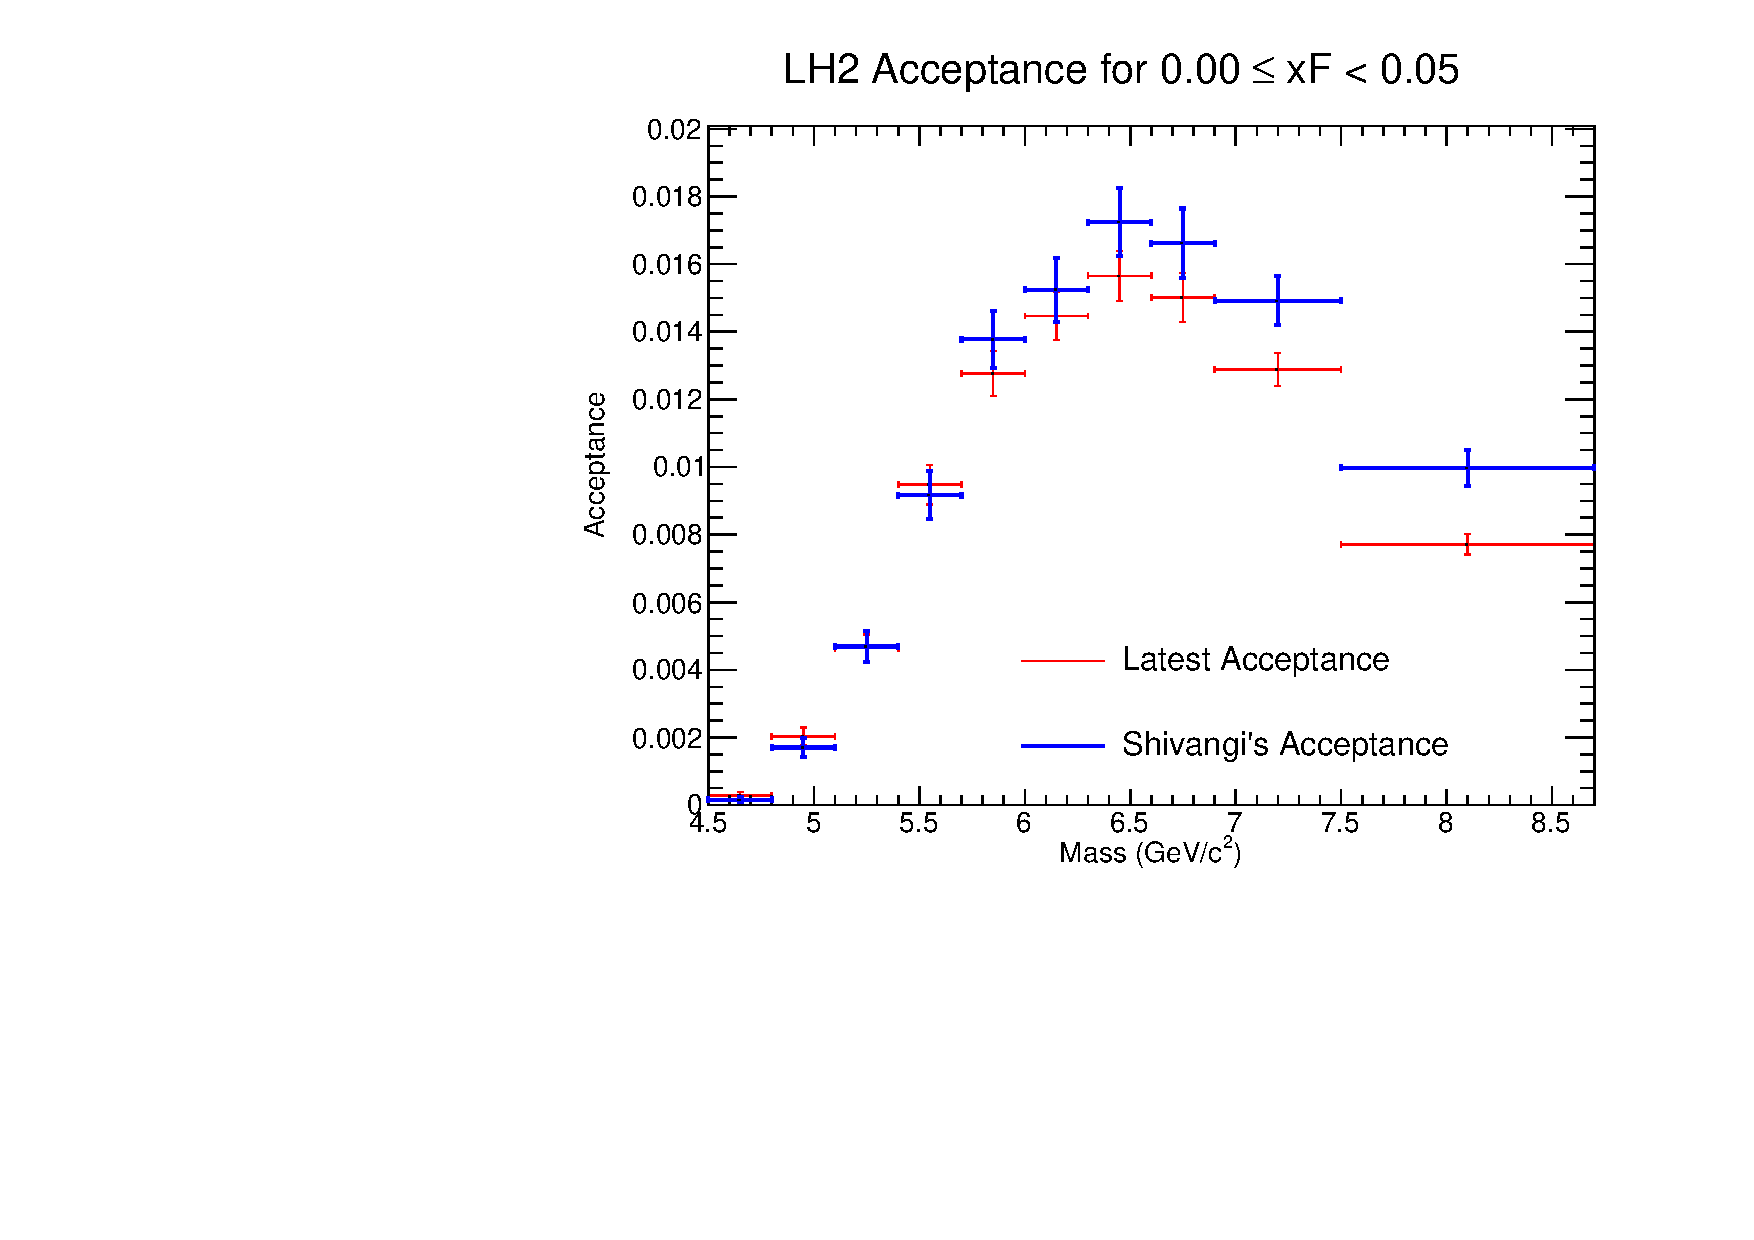
\includegraphics[width=\linewidth]{LH2_acceptance_xF_bin_0.pdf}
       \caption{Acceptance for LH2}
    \end{subfigure}
    \hfill
    \begin{subfigure}[b]{0.48\textwidth}
       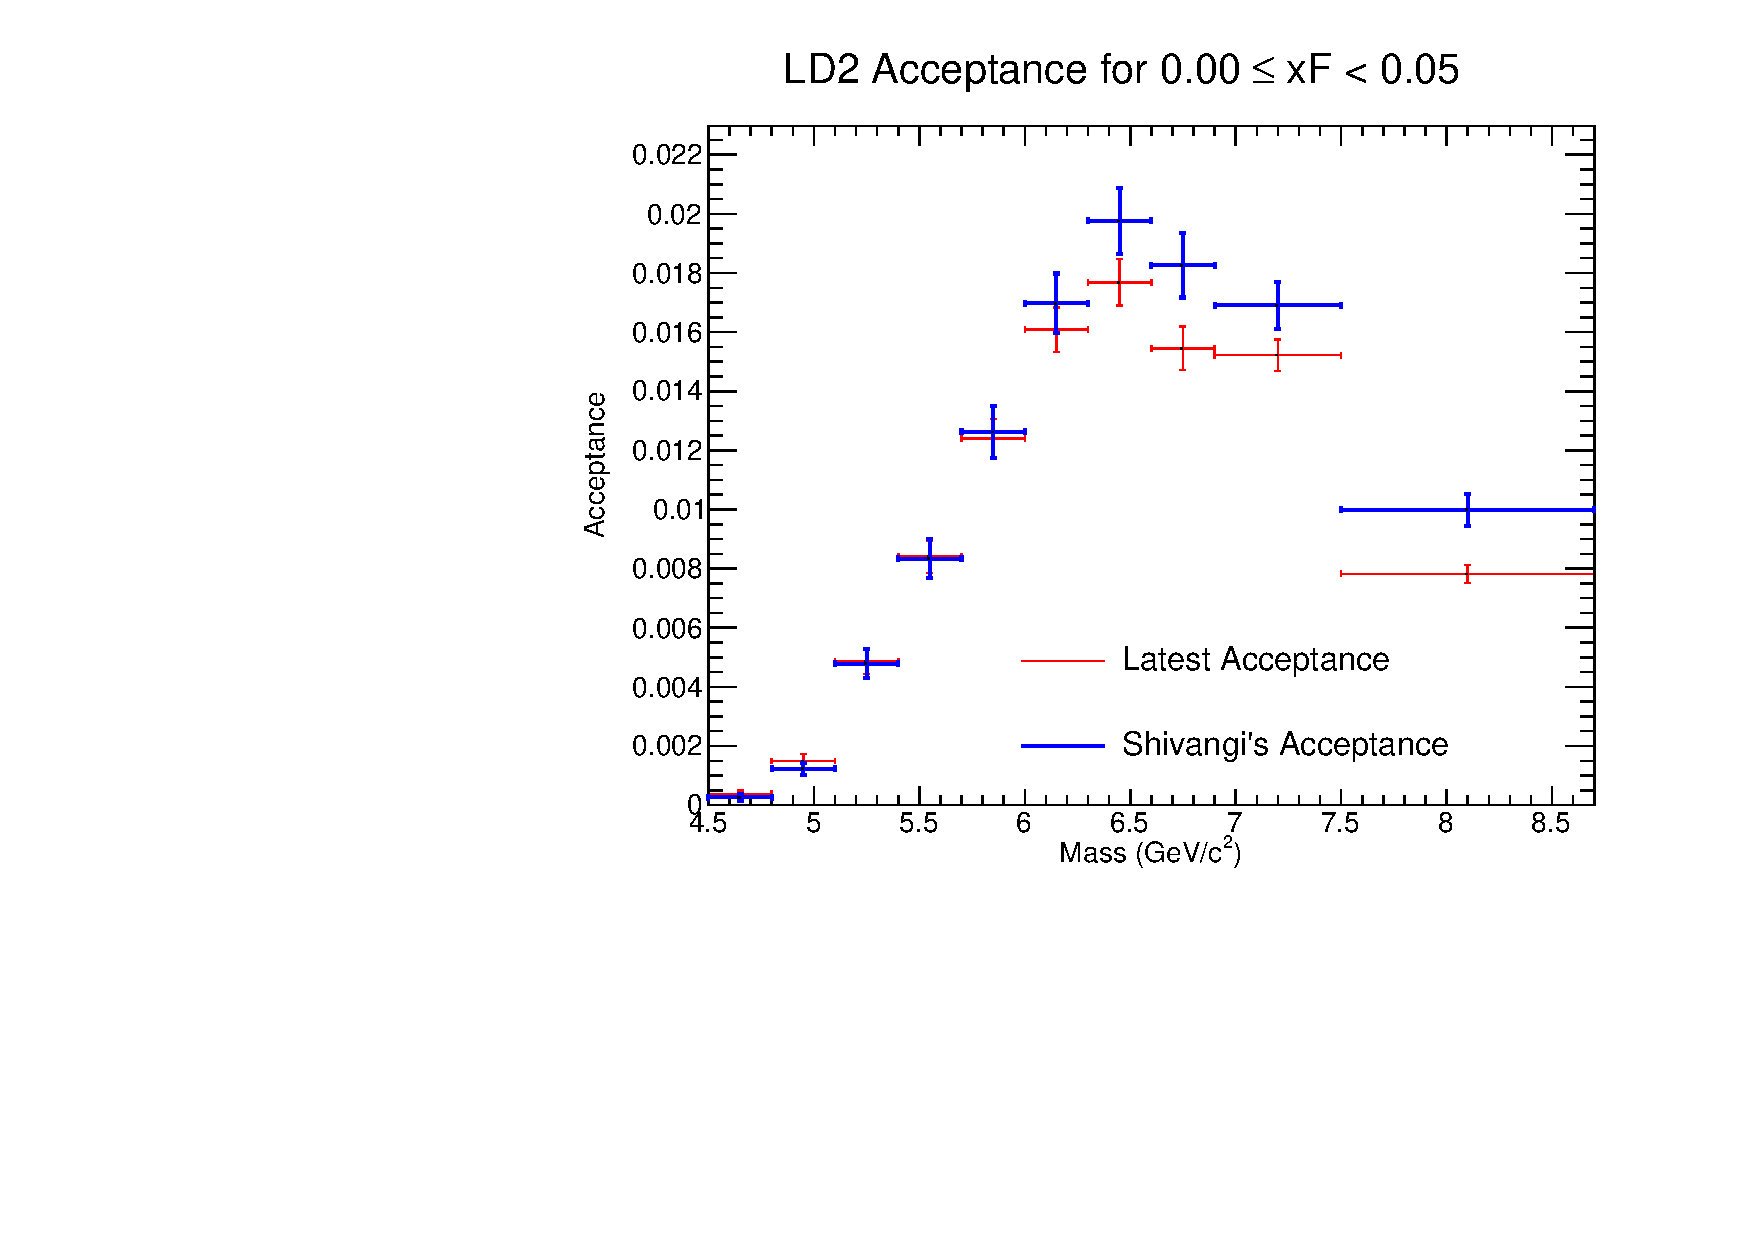
\includegraphics[width=\linewidth]{LD2_acceptance_xF_bin_0.pdf}
       \caption{Acceptance for LD2}
    \end{subfigure}

    \begin{subfigure}[b]{0.48\textwidth}
       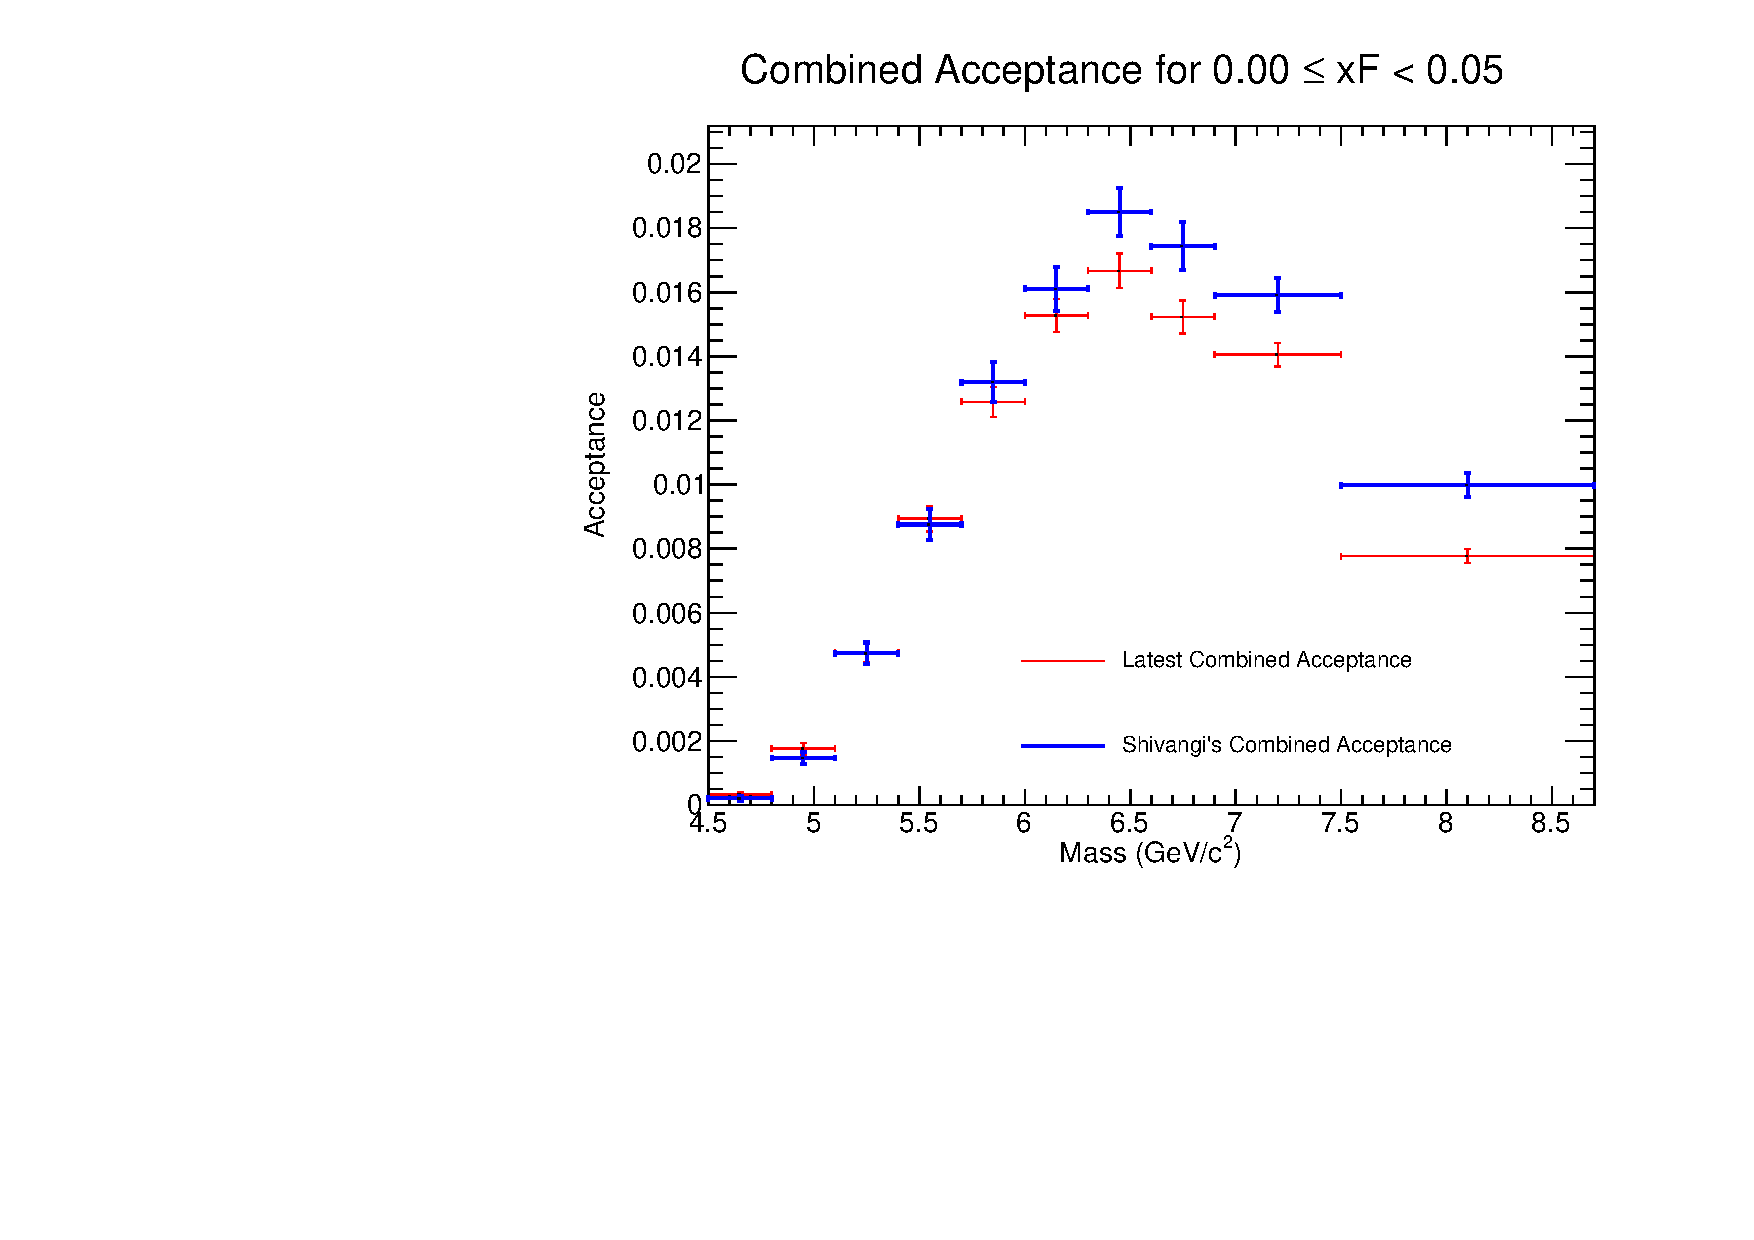
\includegraphics[width=\linewidth]{Combined_acceptance_xF_bin_0.pdf}
       \caption{Combined Acceptance}
    \end{subfigure}
    \hfill
    \begin{subfigure}[b]{0.48\textwidth}
       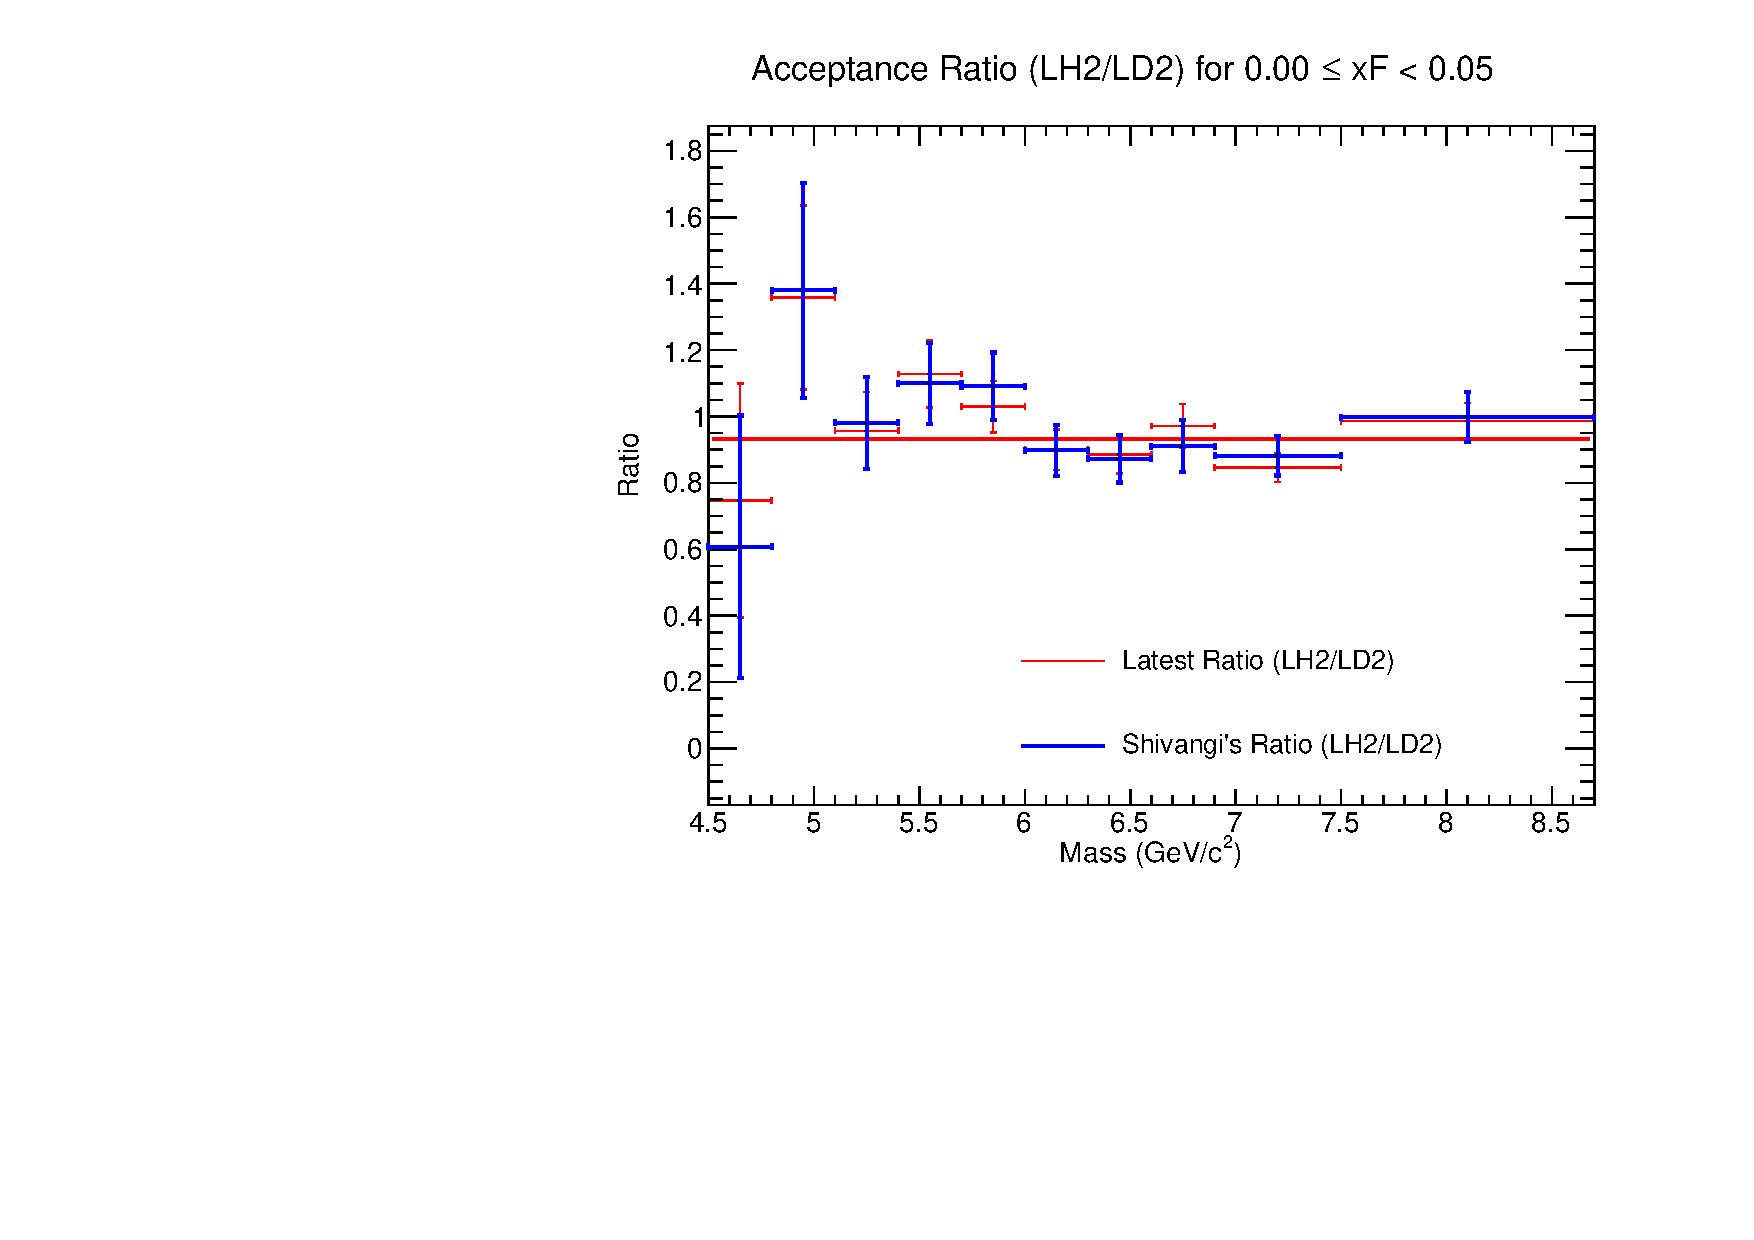
\includegraphics[width=\linewidth]{Acceptance_ratio_xF_bin_0.pdf}
       \caption{Acceptance Ratio (LH2/LD2)}
    \end{subfigure}
    \caption{Acceptance plots for $0.00 \le x_F < 0.05$.}
\end{figure}

\begin{figure}[H]
    \centering
    \begin{subfigure}[b]{0.48\textwidth}
       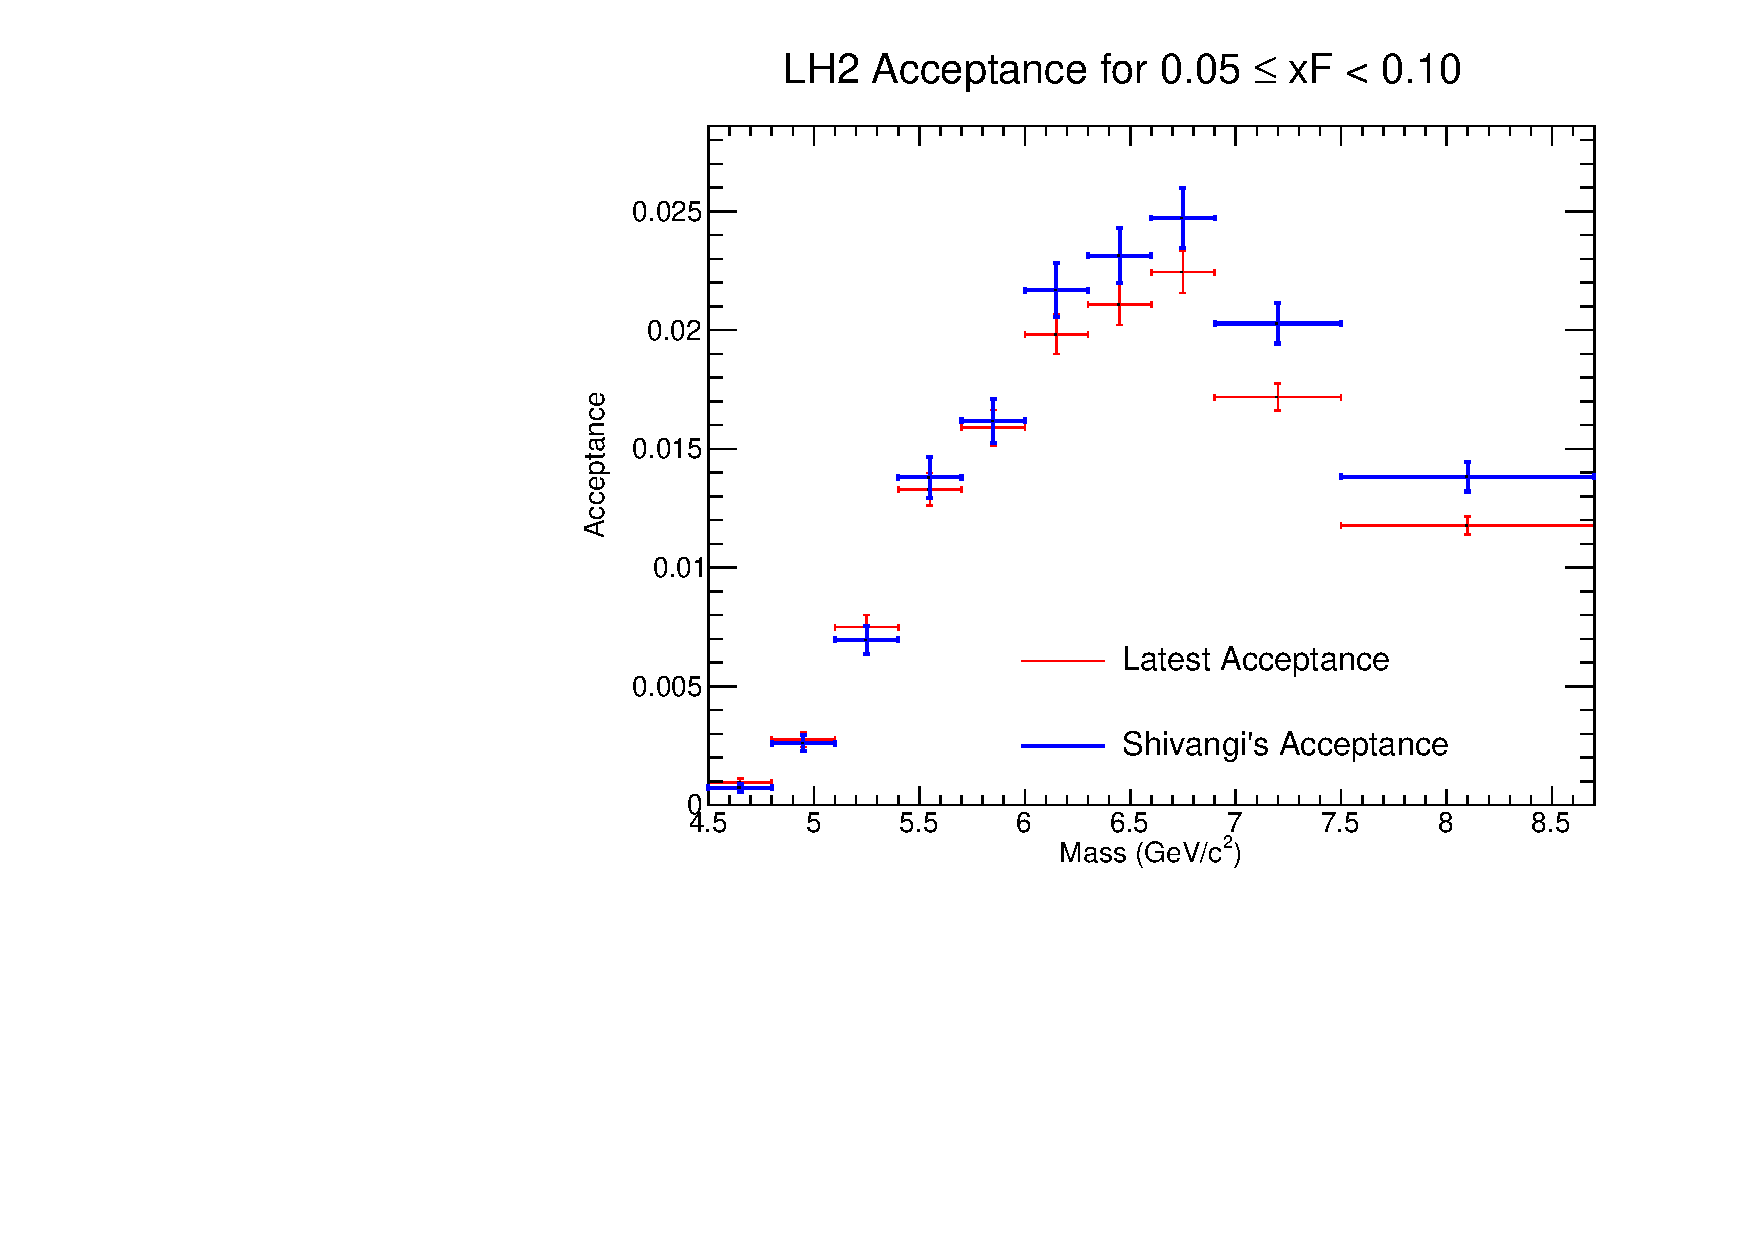
\includegraphics[width=\linewidth]{LH2_acceptance_xF_bin_1.pdf}
       \caption{Acceptance for LH2}
    \end{subfigure}
    \hfill
    \begin{subfigure}[b]{0.48\textwidth}
       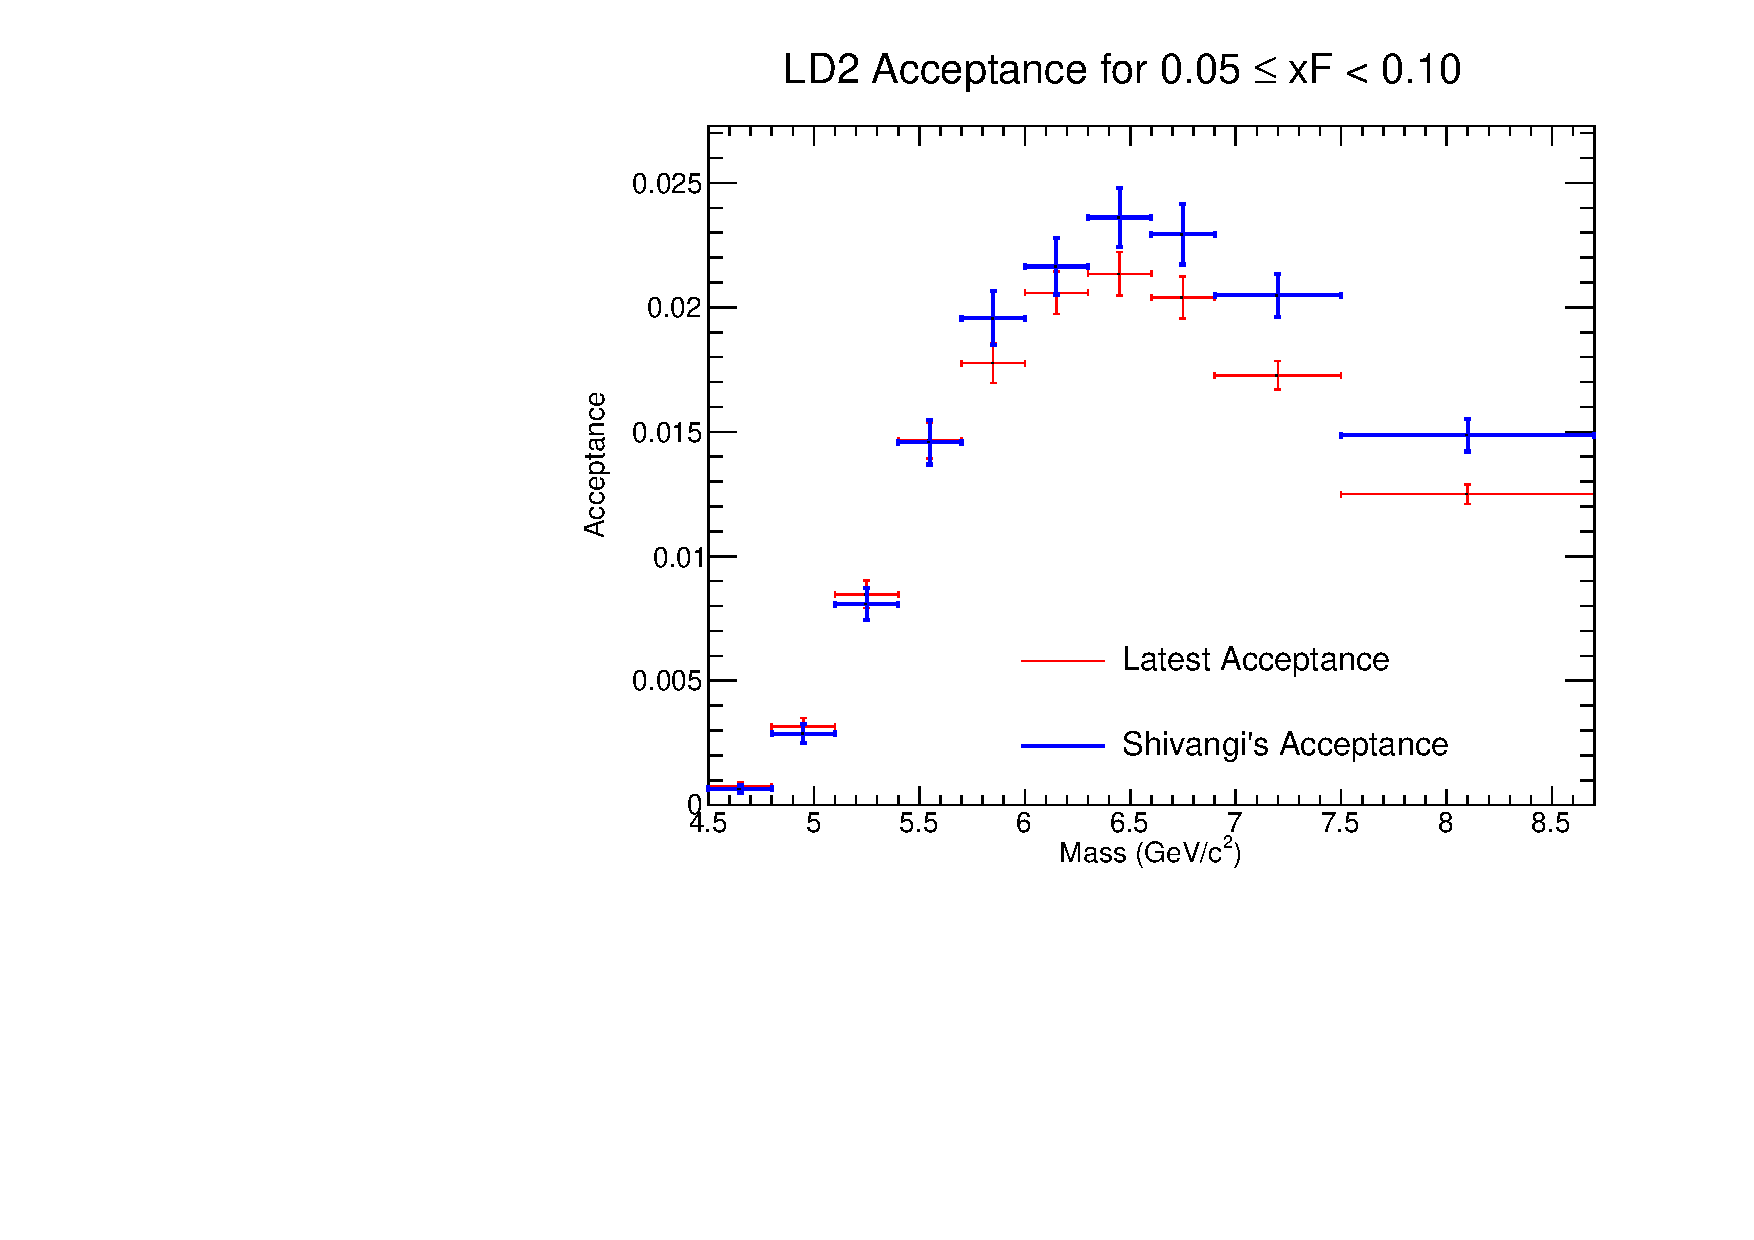
\includegraphics[width=\linewidth]{LD2_acceptance_xF_bin_1.pdf}
       \caption{Acceptance for LD2}
    \end{subfigure}

    \begin{subfigure}[b]{0.48\textwidth}
       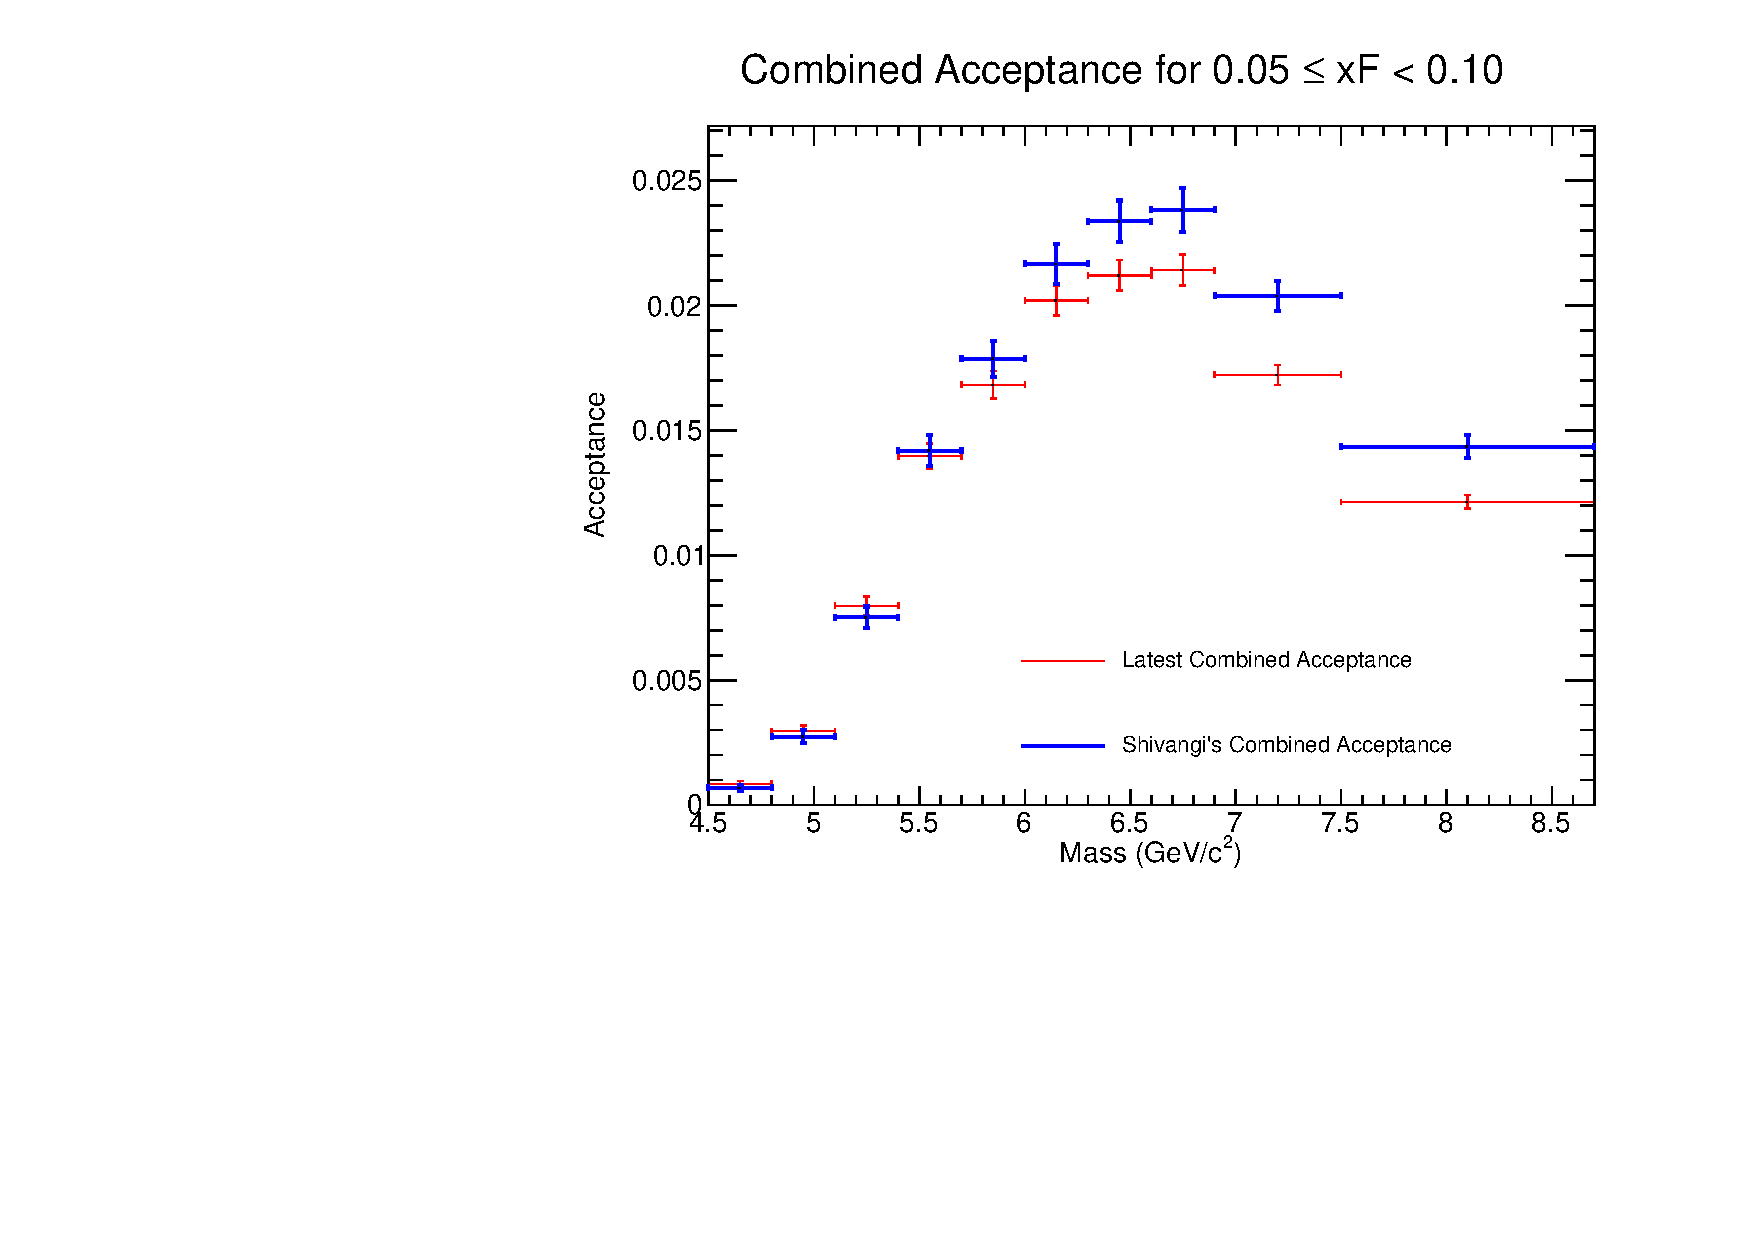
\includegraphics[width=\linewidth]{Combined_acceptance_xF_bin_1.pdf}
       \caption{Combined Acceptance}
    \end{subfigure}
    \hfill
    \begin{subfigure}[b]{0.48\textwidth}
       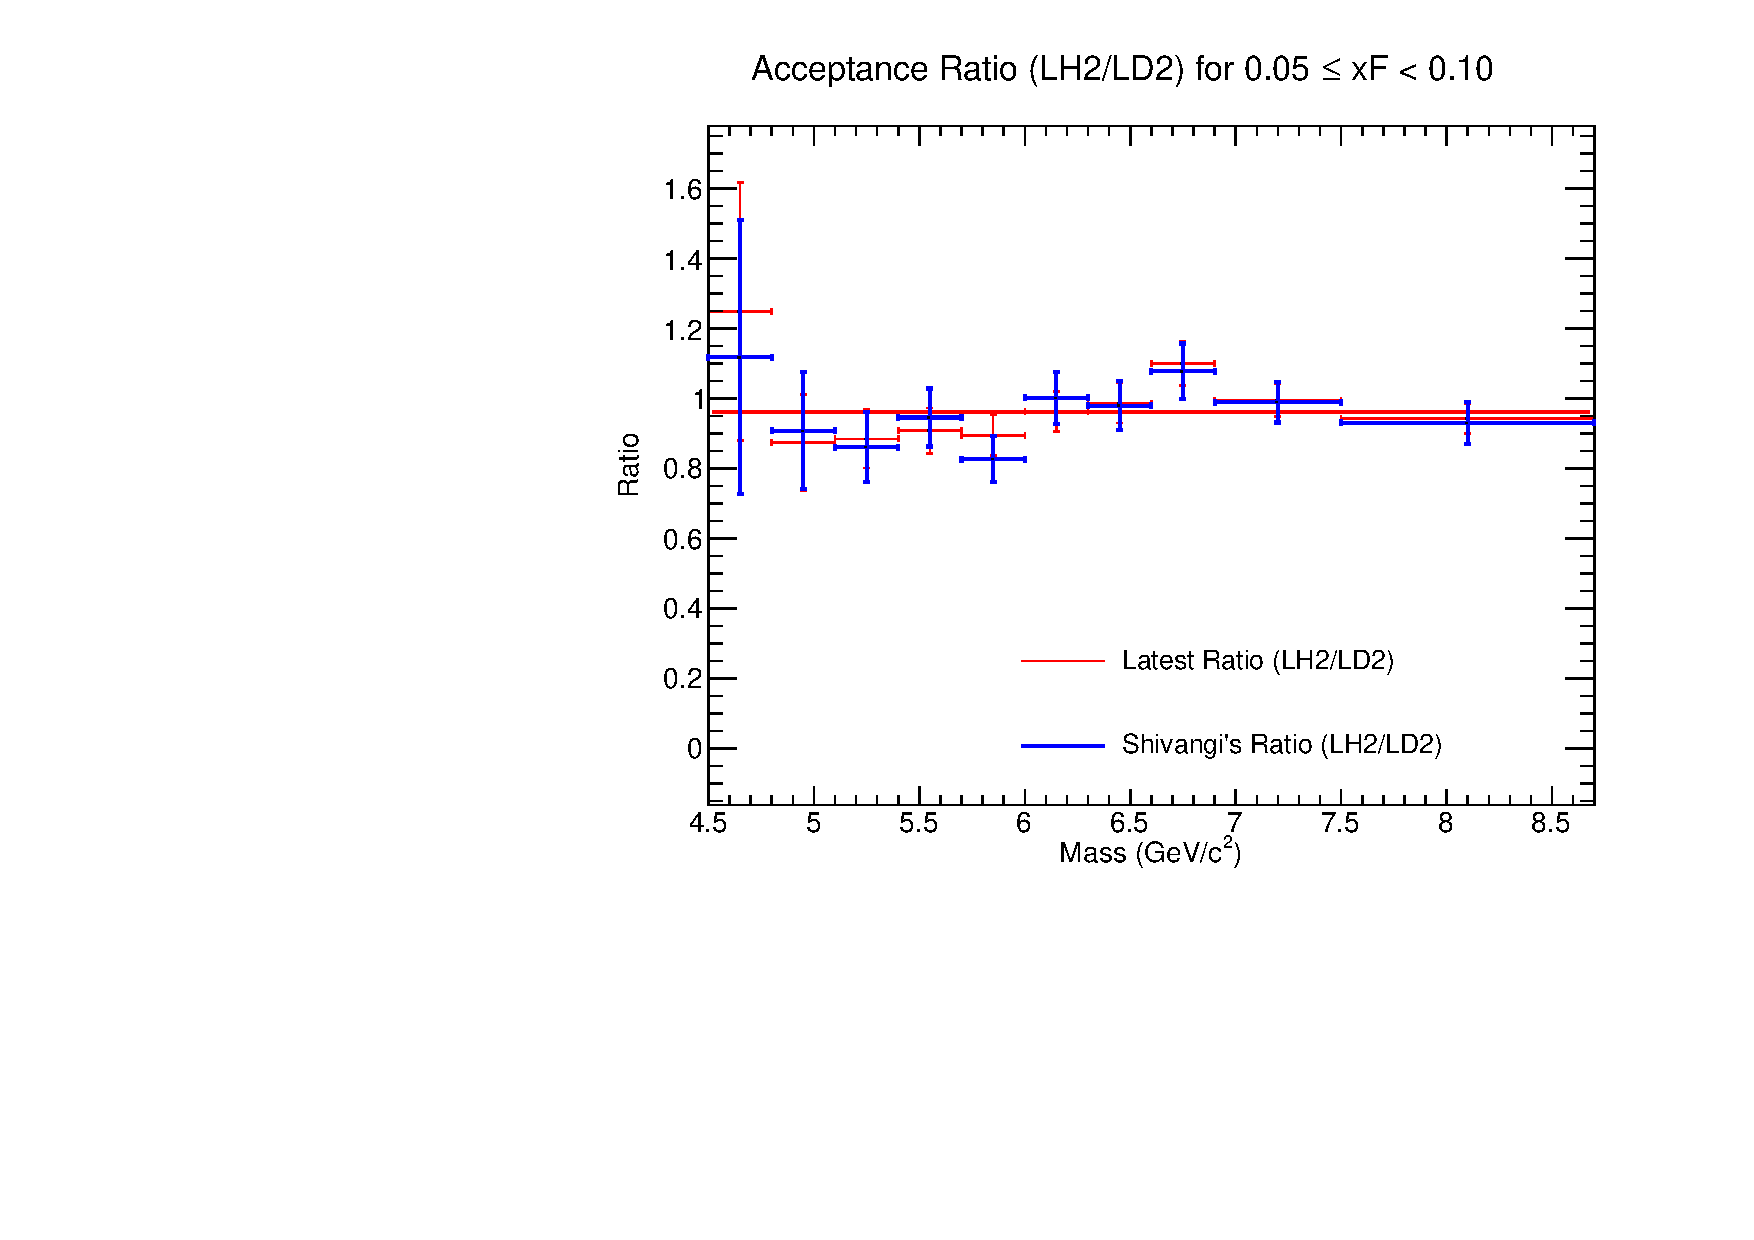
\includegraphics[width=\linewidth]{Acceptance_ratio_xF_bin_1.pdf}
       \caption{Acceptance Ratio (LH2/LD2)}
    \end{subfigure}
    \caption{Acceptance plots for $0.05 \le x_F < 0.10$.}
\end{figure}

\begin{figure}[H]
    \centering
    \begin{subfigure}[b]{0.48\textwidth}
       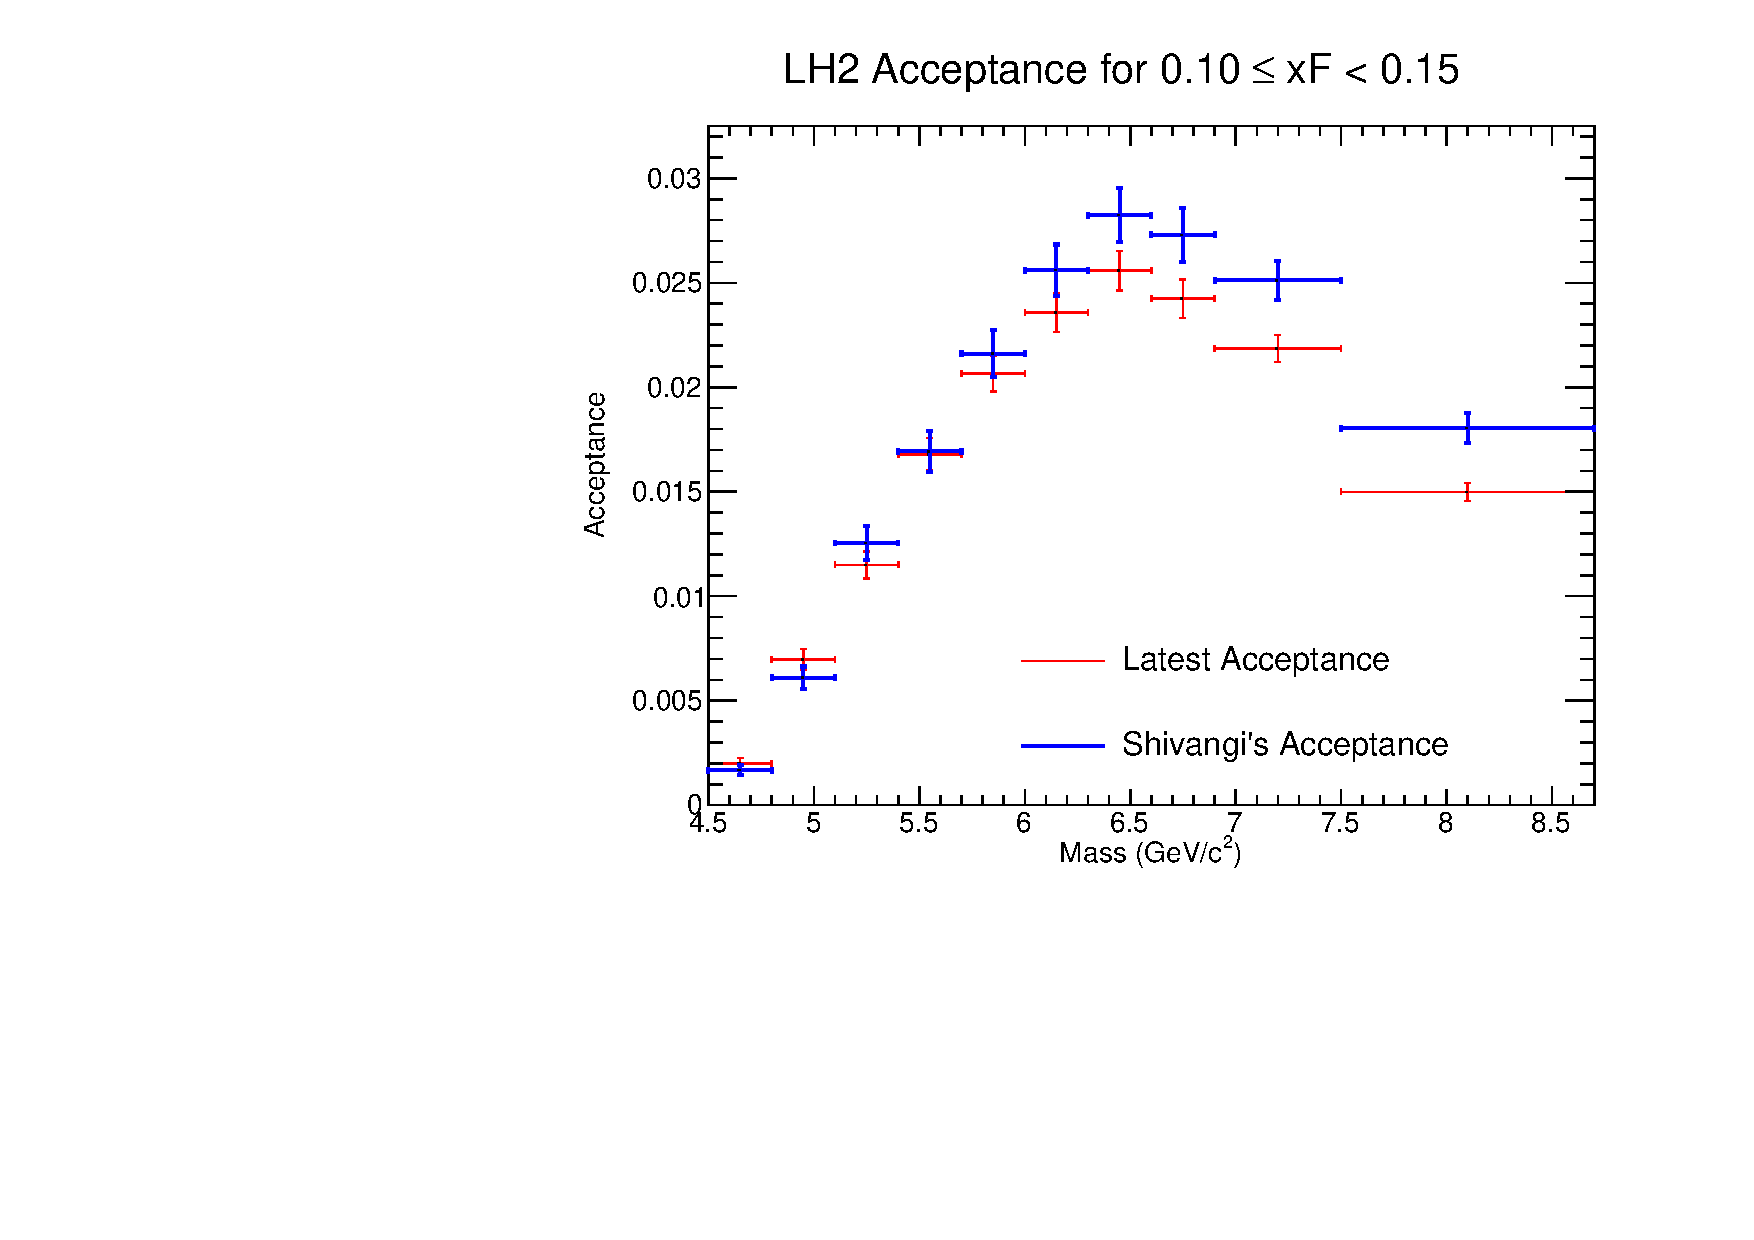
\includegraphics[width=\linewidth]{LH2_acceptance_xF_bin_2.pdf}
       \caption{Acceptance for LH2}
    \end{subfigure}
    \hfill
    \begin{subfigure}[b]{0.48\textwidth}
       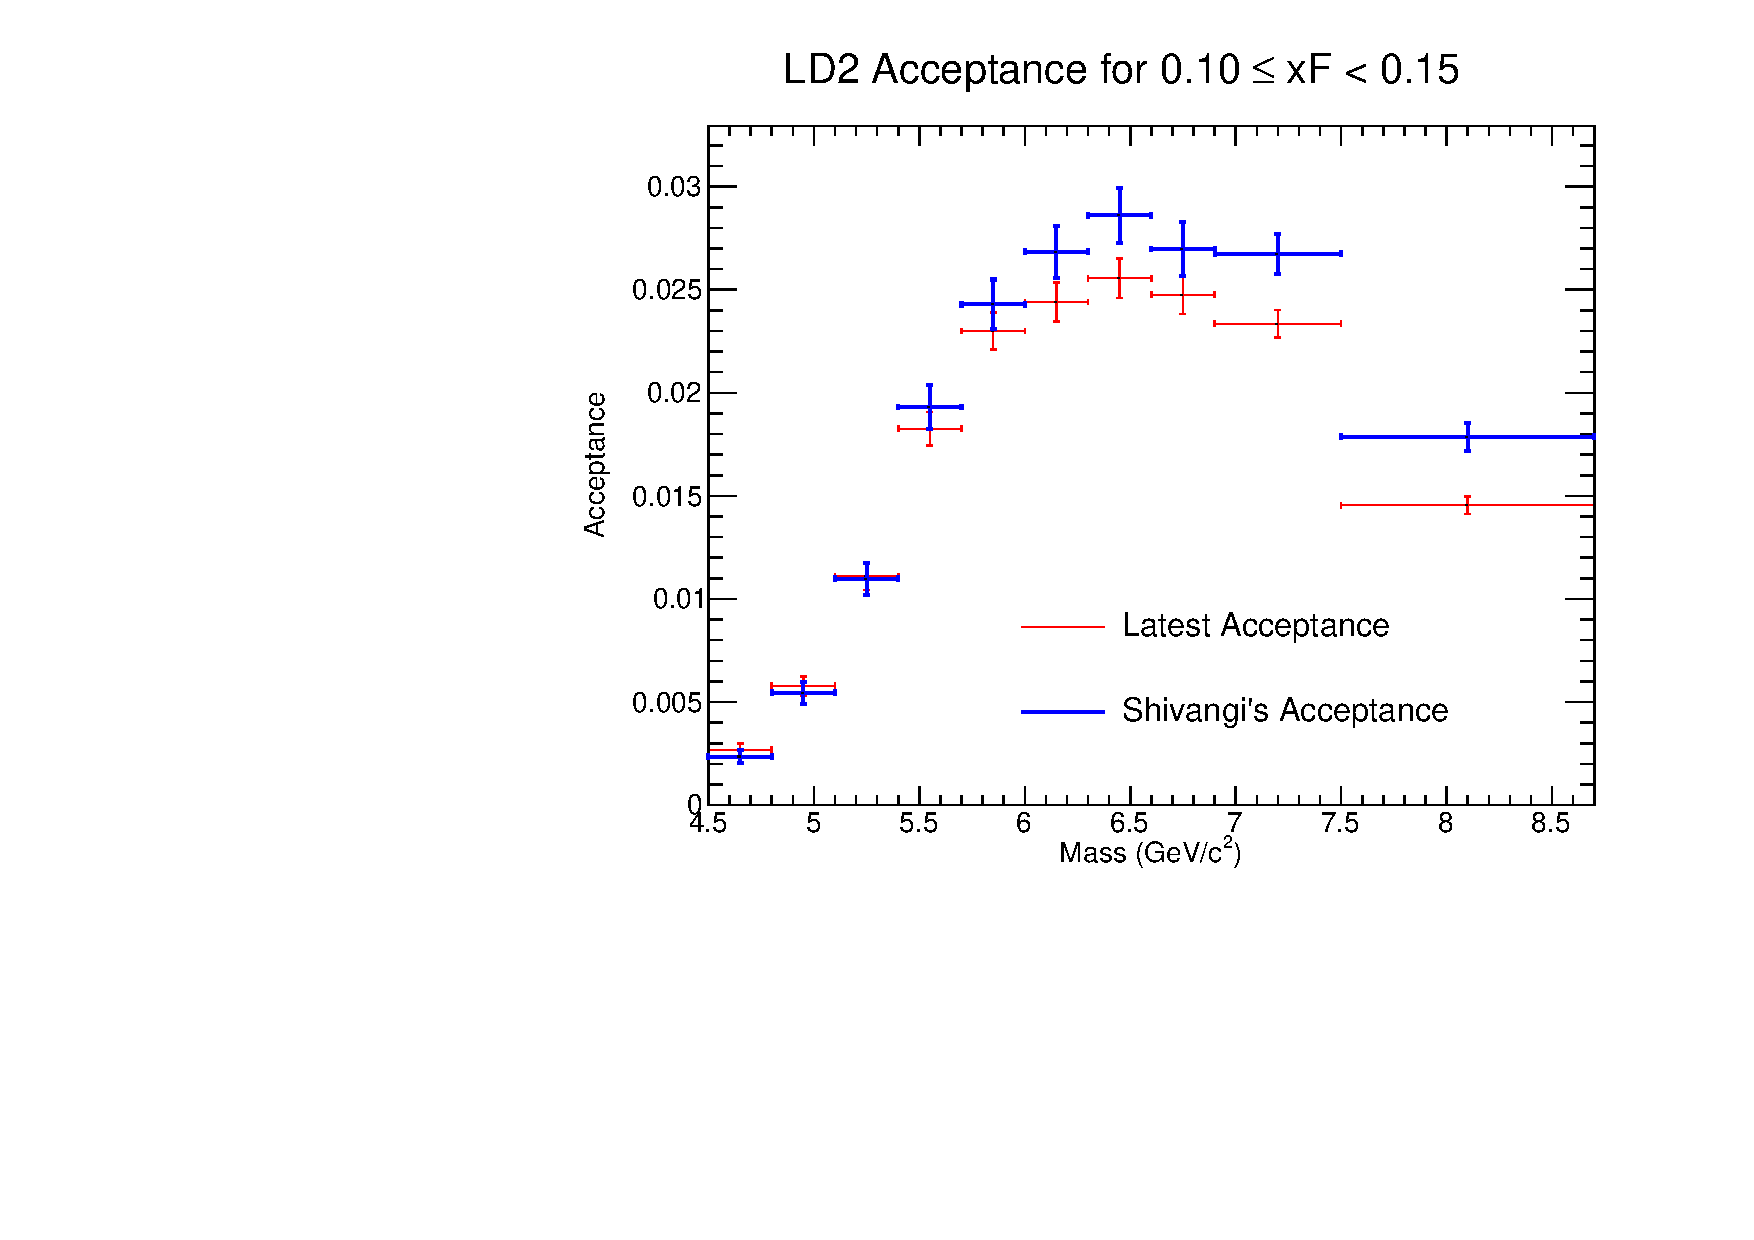
\includegraphics[width=\linewidth]{LD2_acceptance_xF_bin_2.pdf}
       \caption{Acceptance for LD2}
    \end{subfigure}

    \begin{subfigure}[b]{0.48\textwidth}
       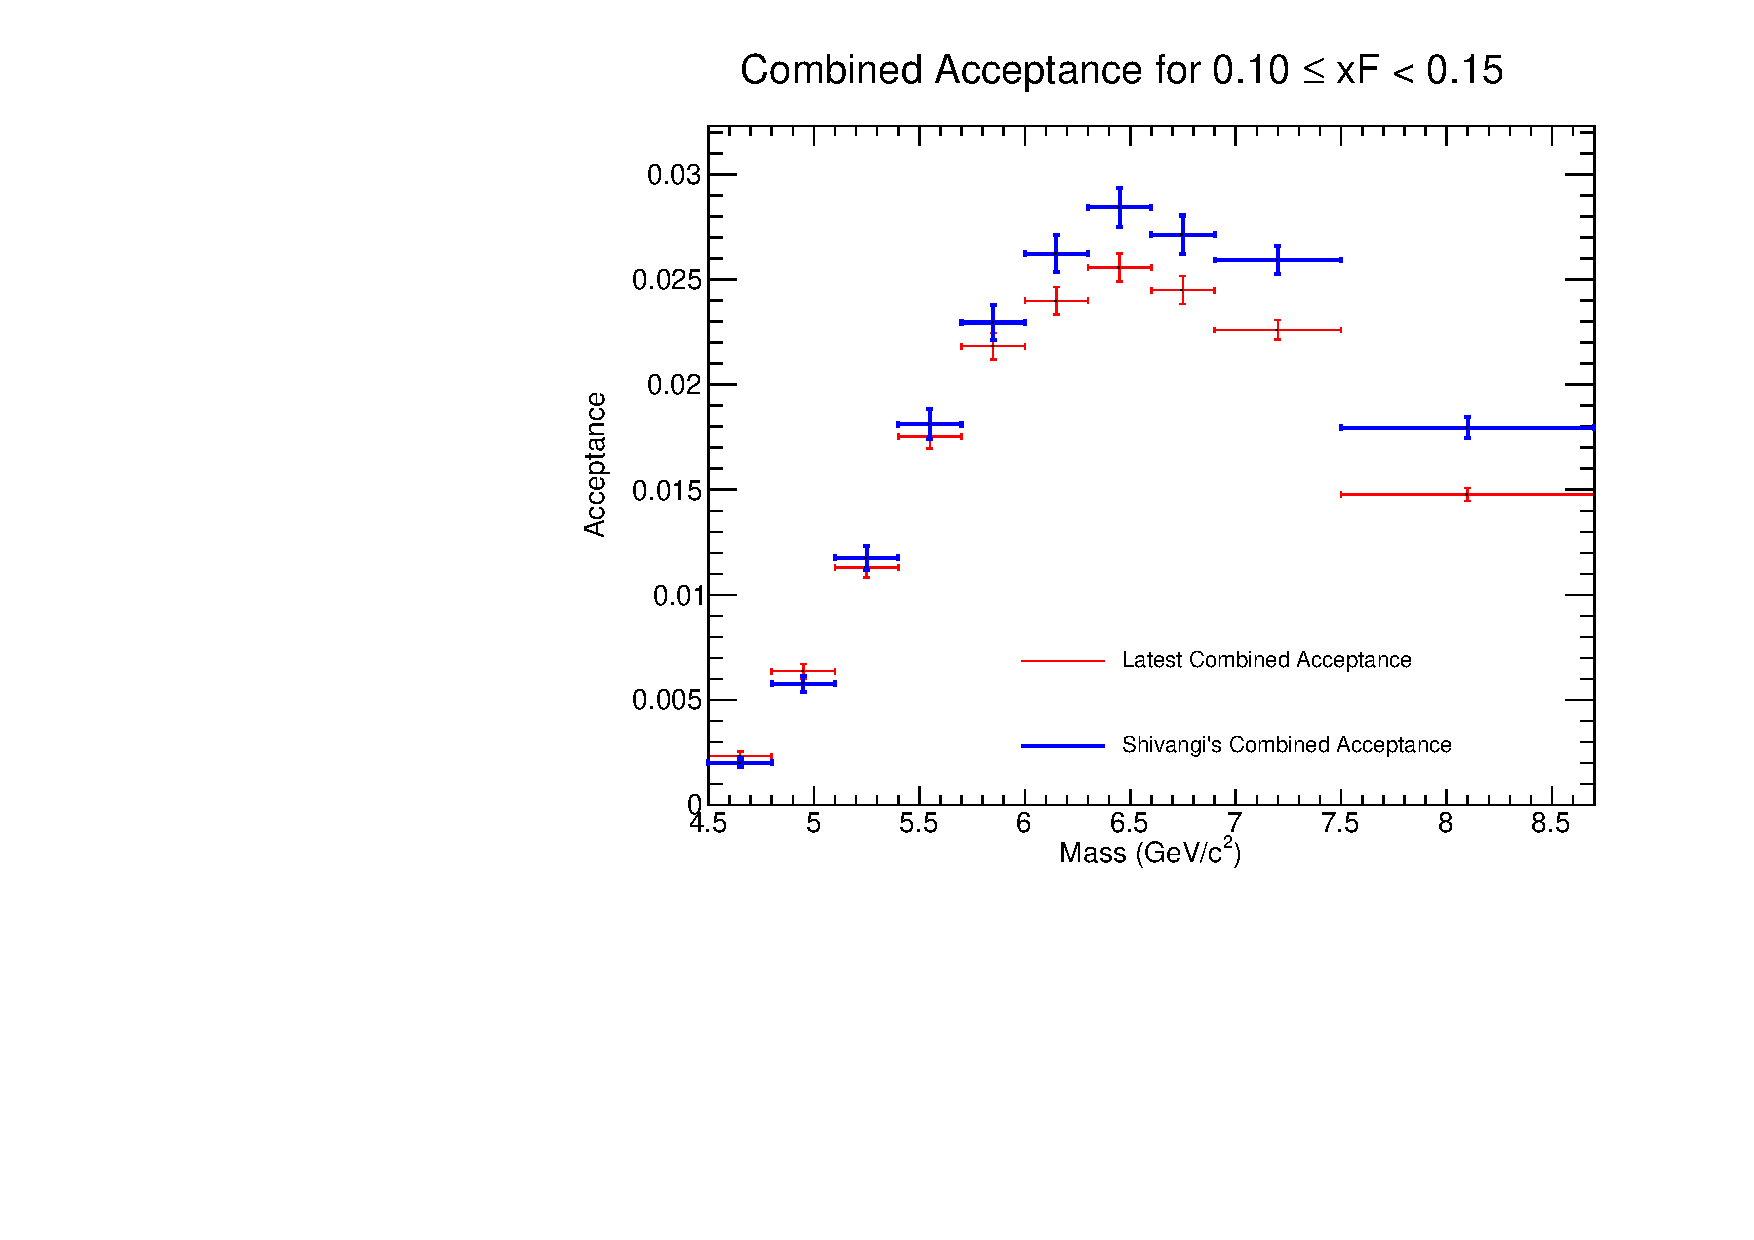
\includegraphics[width=\linewidth]{Combined_acceptance_xF_bin_2.pdf}
       \caption{Combined Acceptance}
    \end{subfigure}
    \hfill
    \begin{subfigure}[b]{0.48\textwidth}
       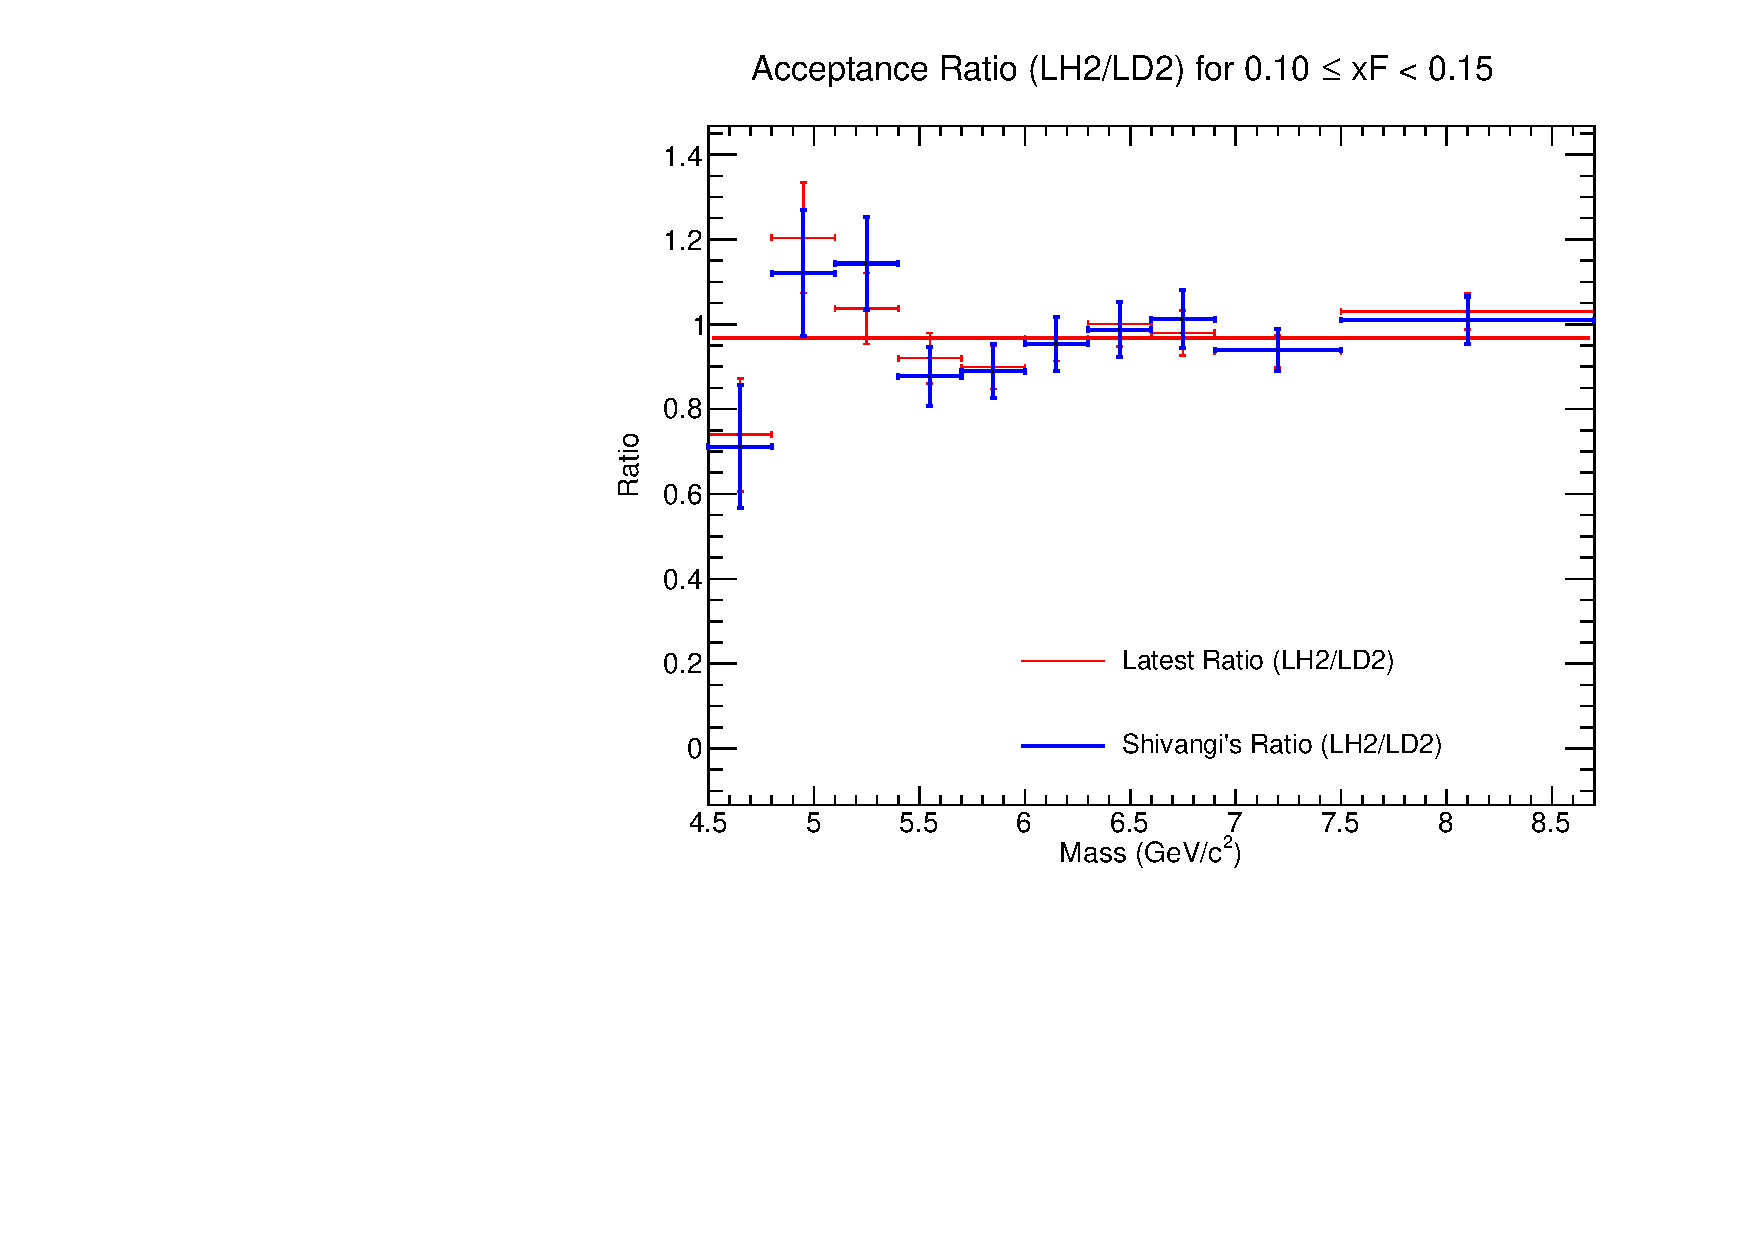
\includegraphics[width=\linewidth]{Acceptance_ratio_xF_bin_2.pdf}
       \caption{Acceptance Ratio (LH2/LD2)}
    \end{subfigure}
    \caption{Acceptance plots for $0.10 \le x_F < 0.15$.}
\end{figure}

\begin{figure}[H]
    \centering
    \begin{subfigure}[b]{0.48\textwidth}
       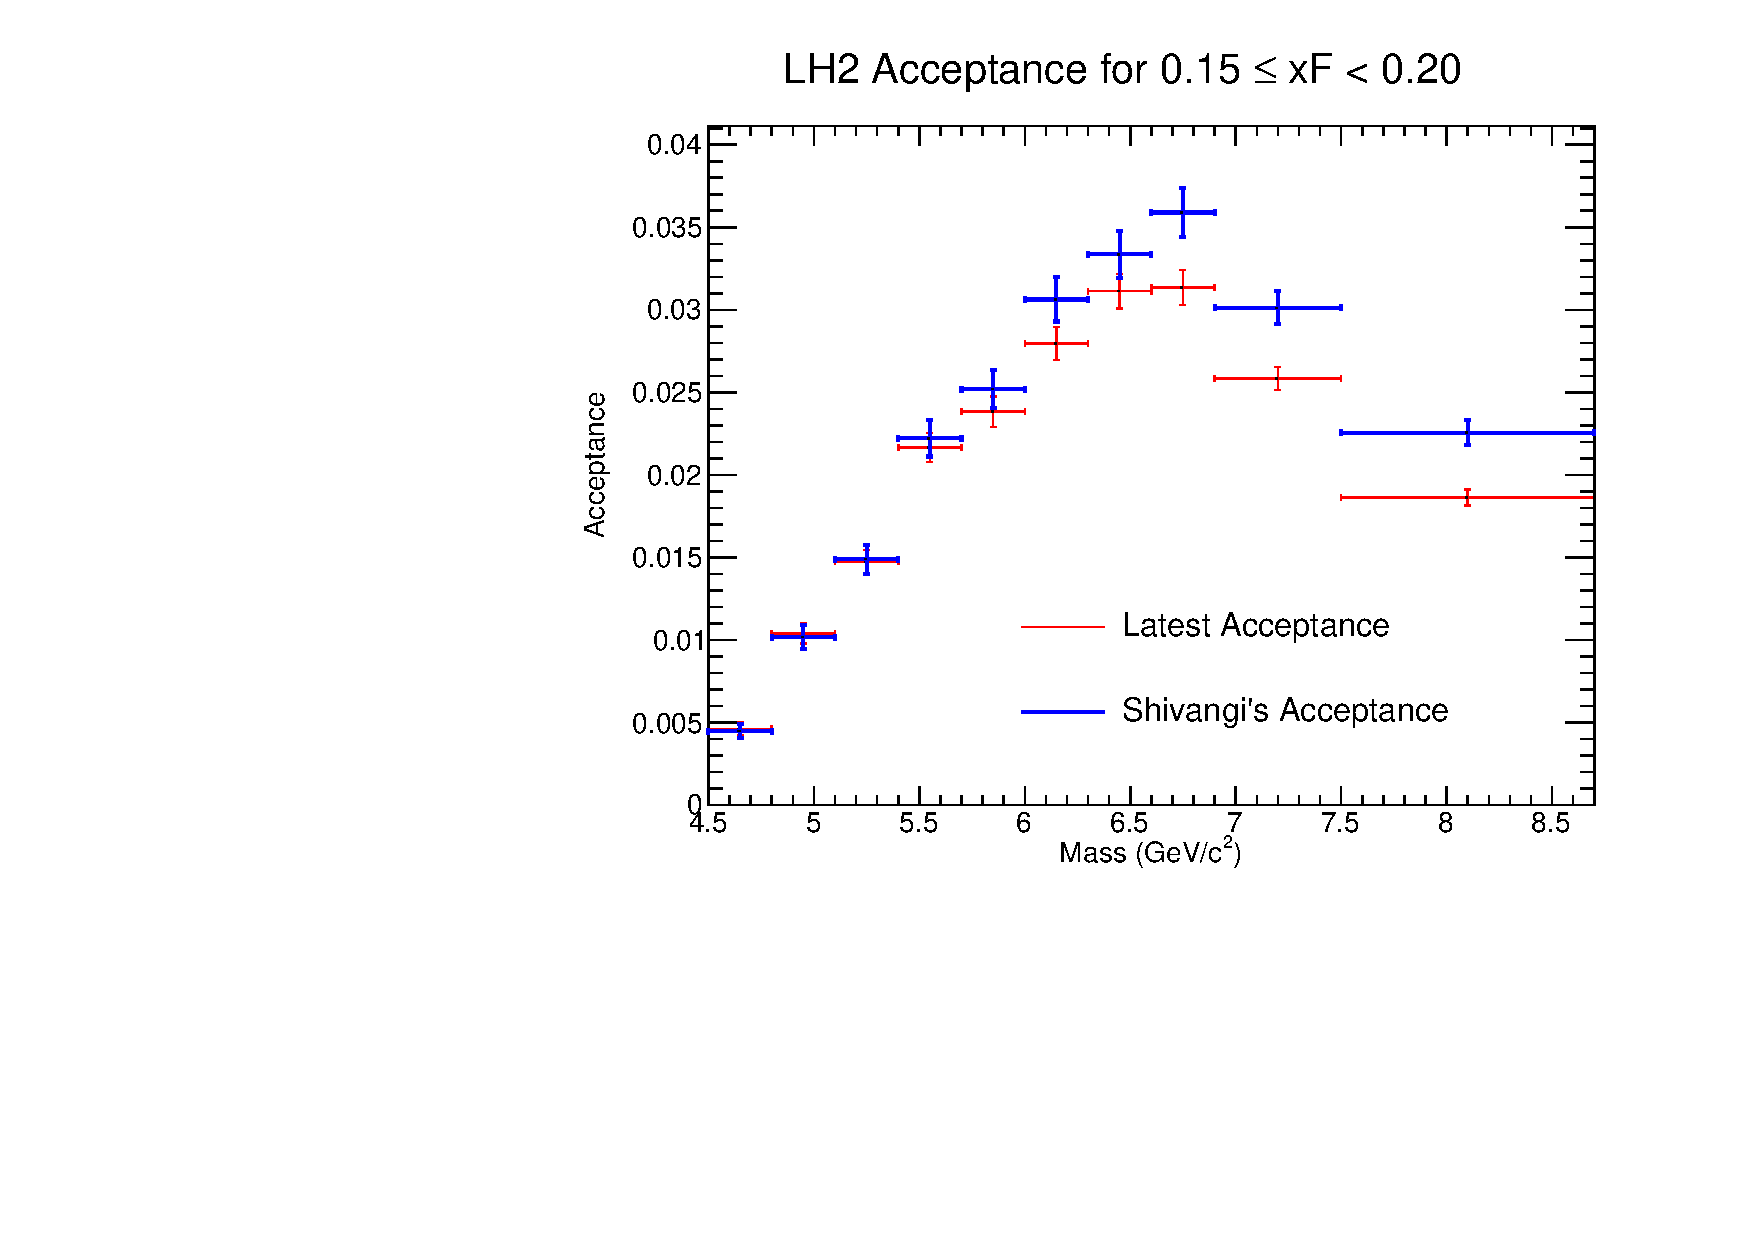
\includegraphics[width=\linewidth]{LH2_acceptance_xF_bin_3.pdf}
       \caption{Acceptance for LH2}
    \end{subfigure}
    \hfill
    \begin{subfigure}[b]{0.48\textwidth}
       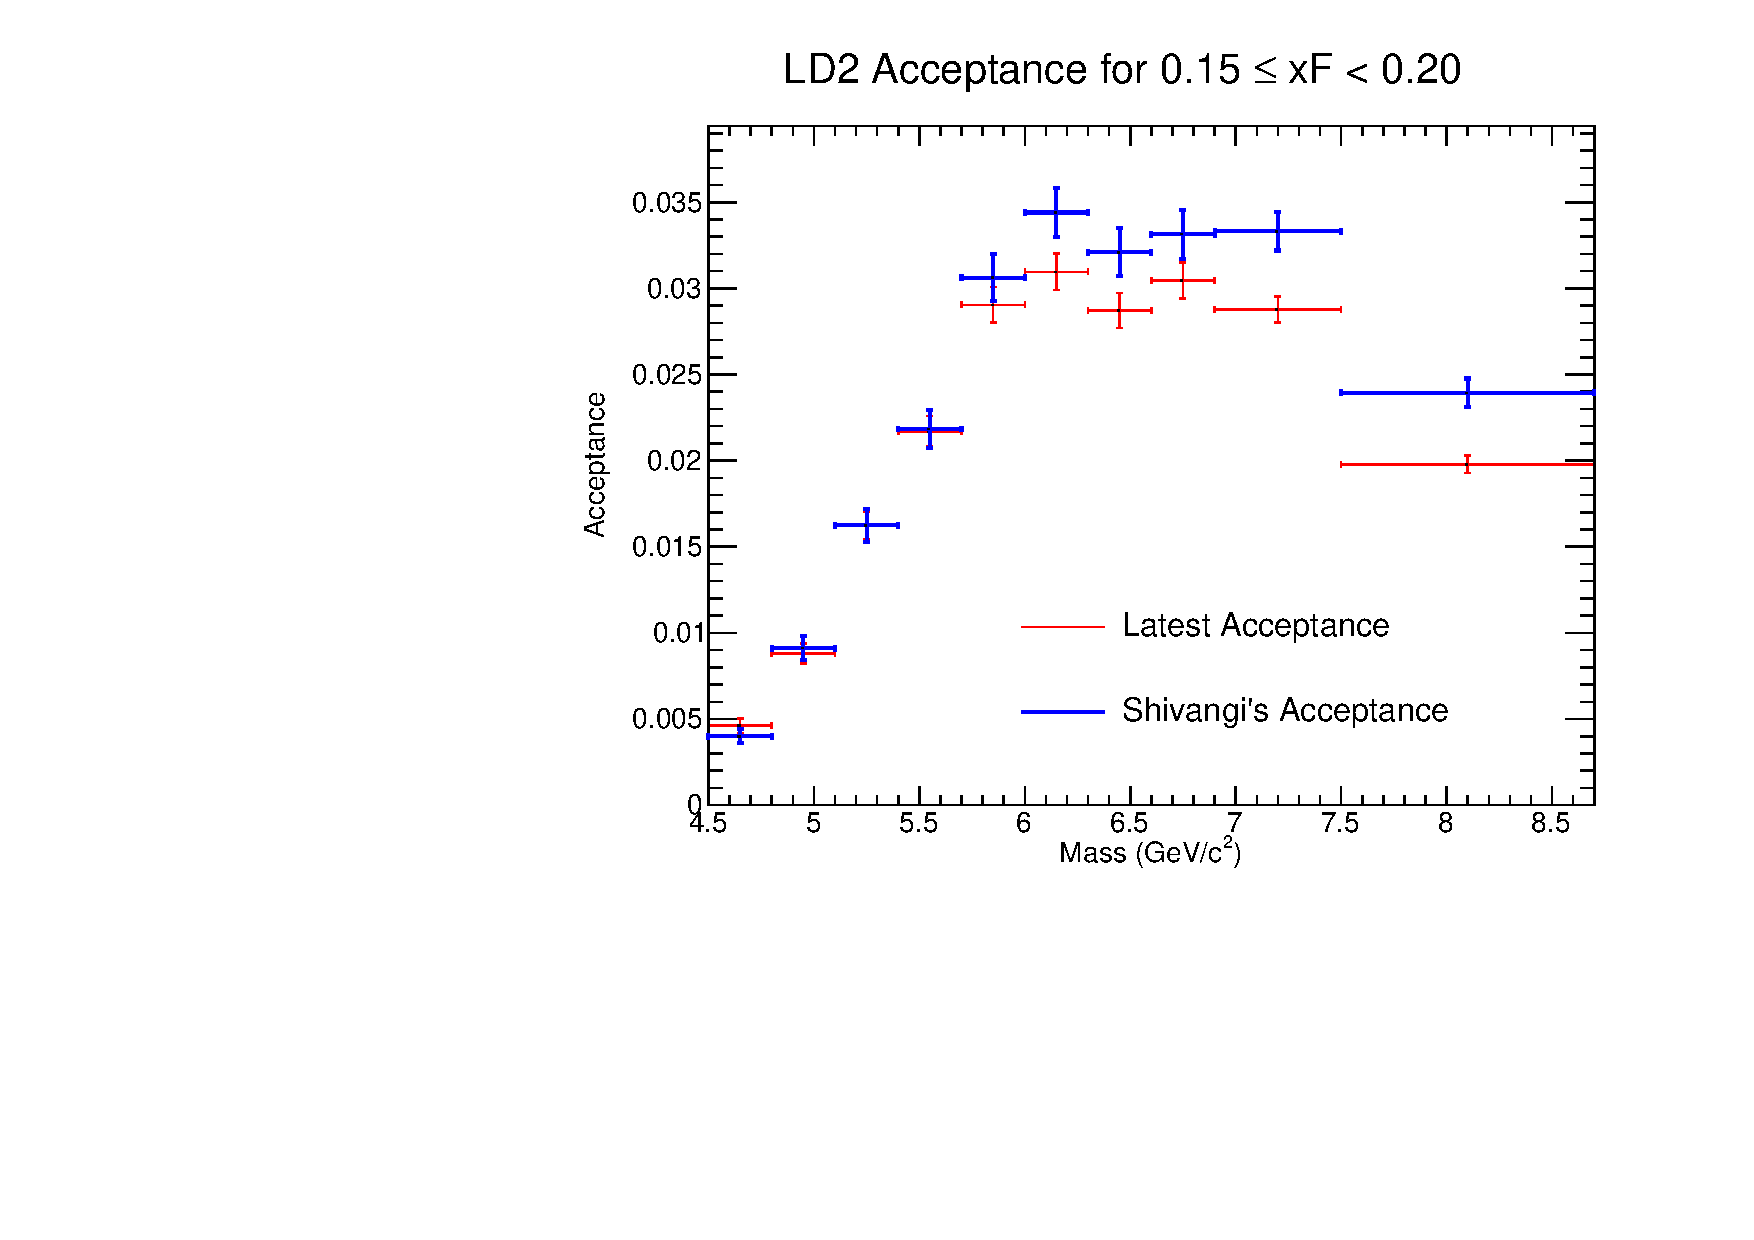
\includegraphics[width=\linewidth]{LD2_acceptance_xF_bin_3.pdf}
       \caption{Acceptance for LD2}
    \end{subfigure}

    \begin{subfigure}[b]{0.48\textwidth}
       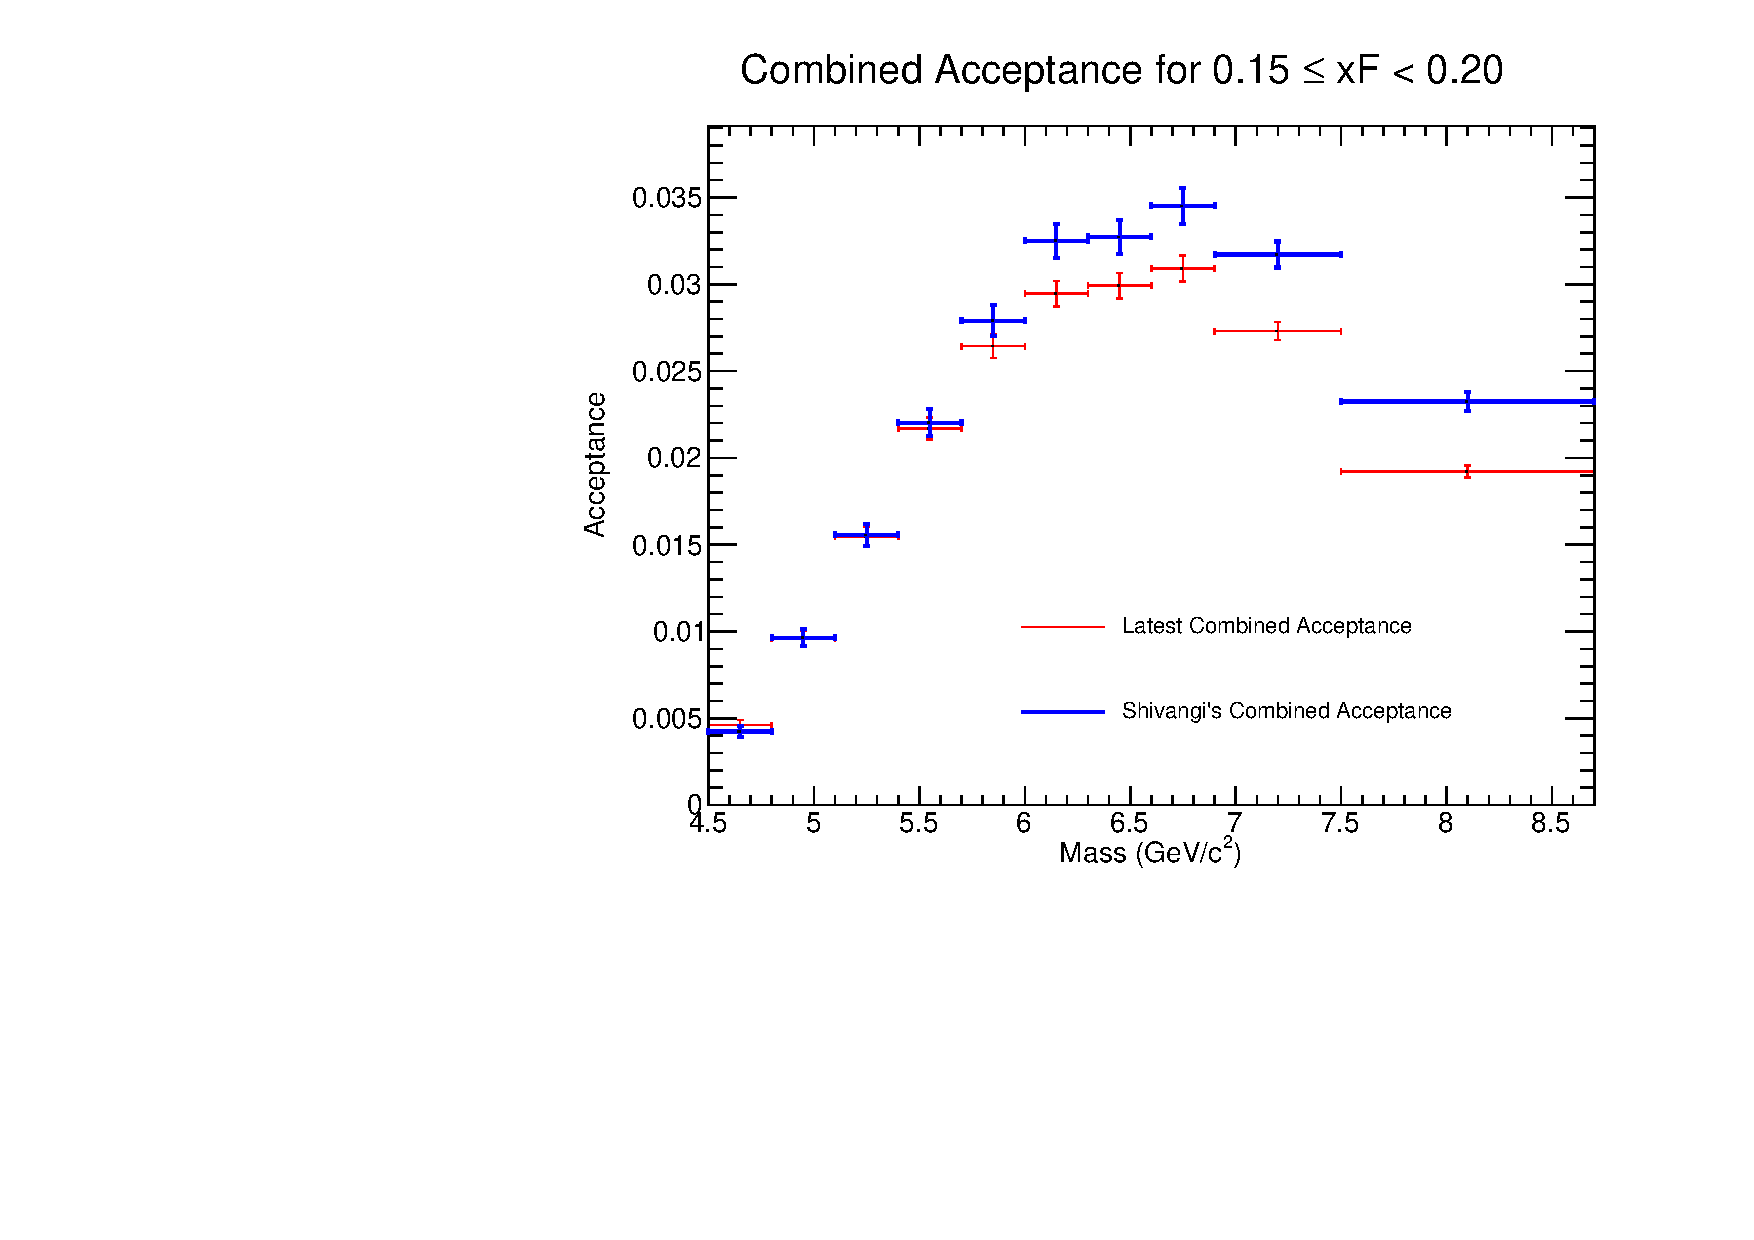
\includegraphics[width=\linewidth]{Combined_acceptance_xF_bin_3.pdf}
       \caption{Combined Acceptance}
    \end{subfigure}
    \hfill
    \begin{subfigure}[b]{0.48\textwidth}
       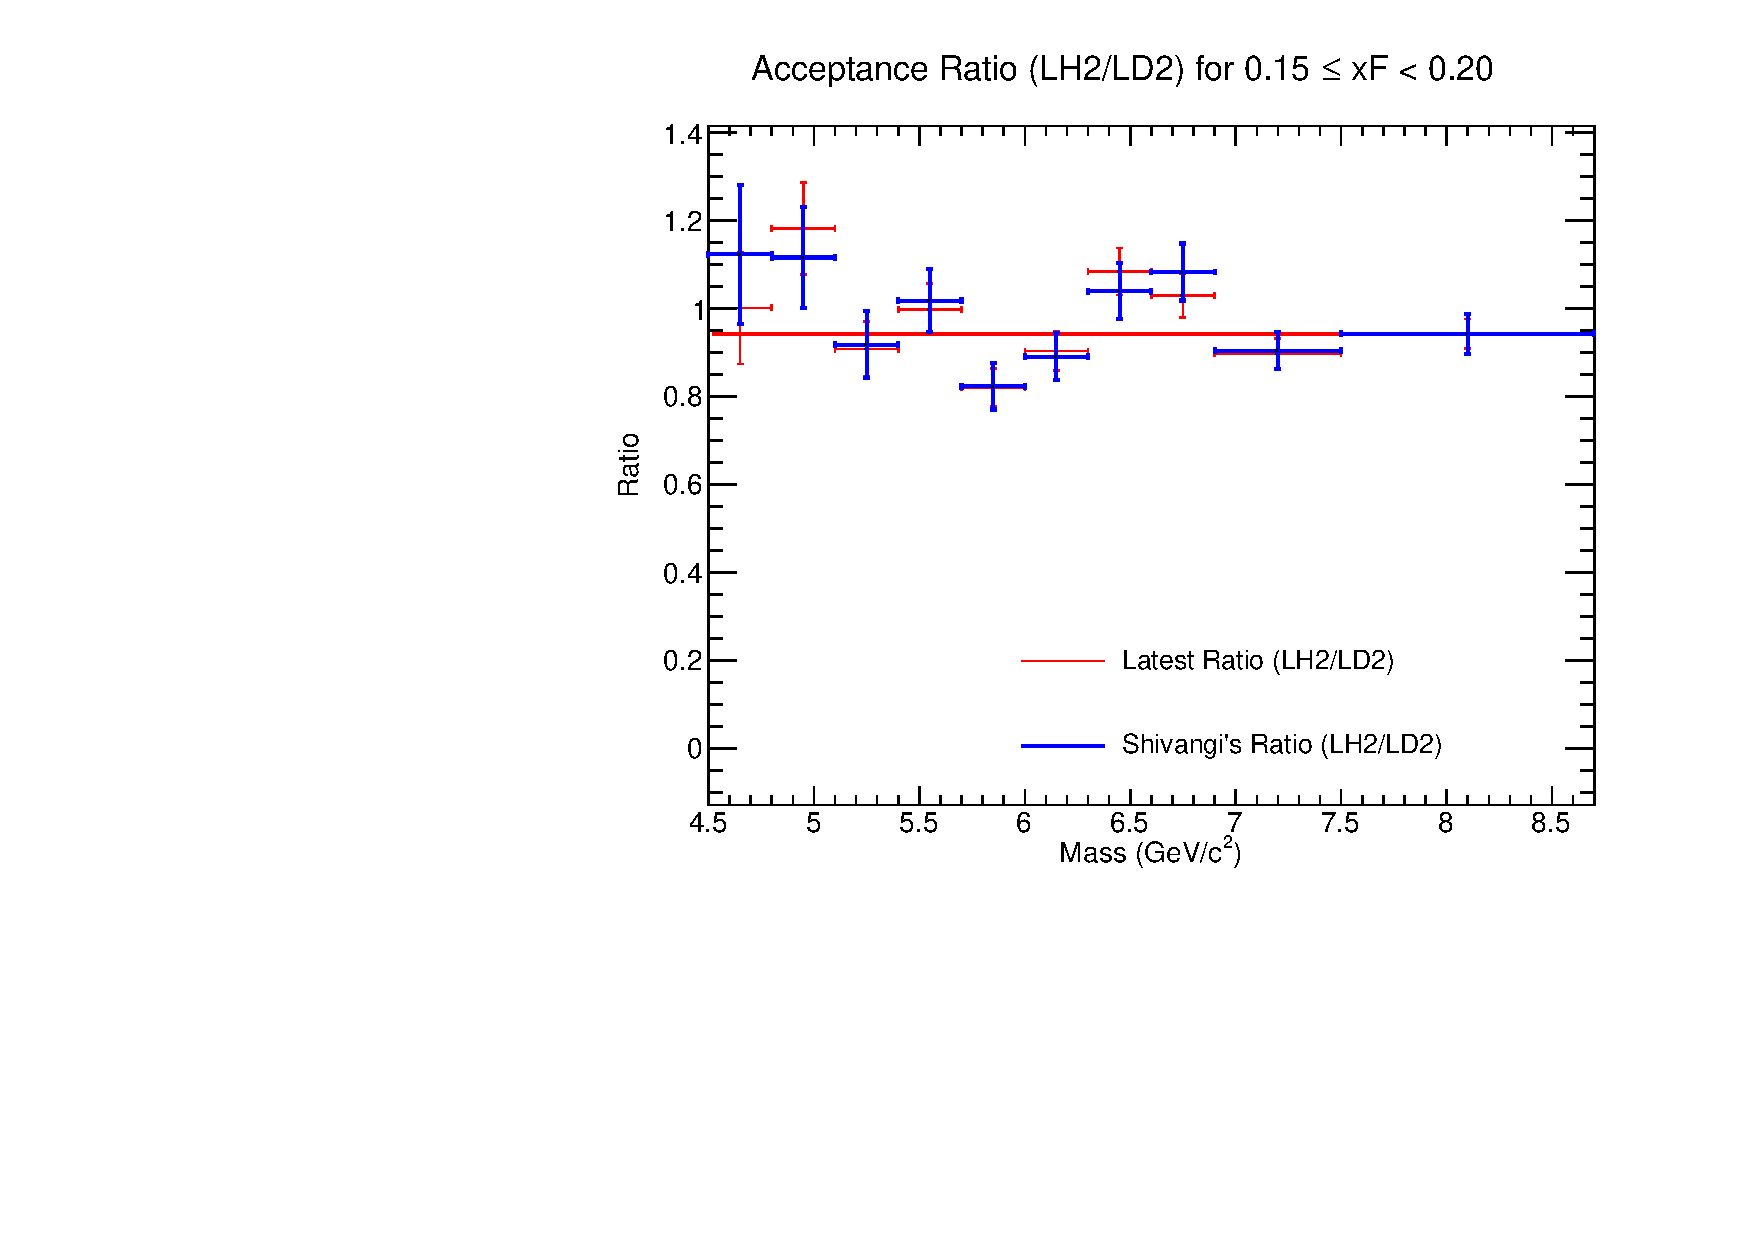
\includegraphics[width=\linewidth]{Acceptance_ratio_xF_bin_3.pdf}
       \caption{Acceptance Ratio (LH2/LD2)}
    \end{subfigure}
    \caption{Acceptance plots for $0.15 \le x_F < 0.20$.}
\end{figure}

\begin{figure}[H]
    \centering
    \begin{subfigure}[b]{0.48\textwidth}
       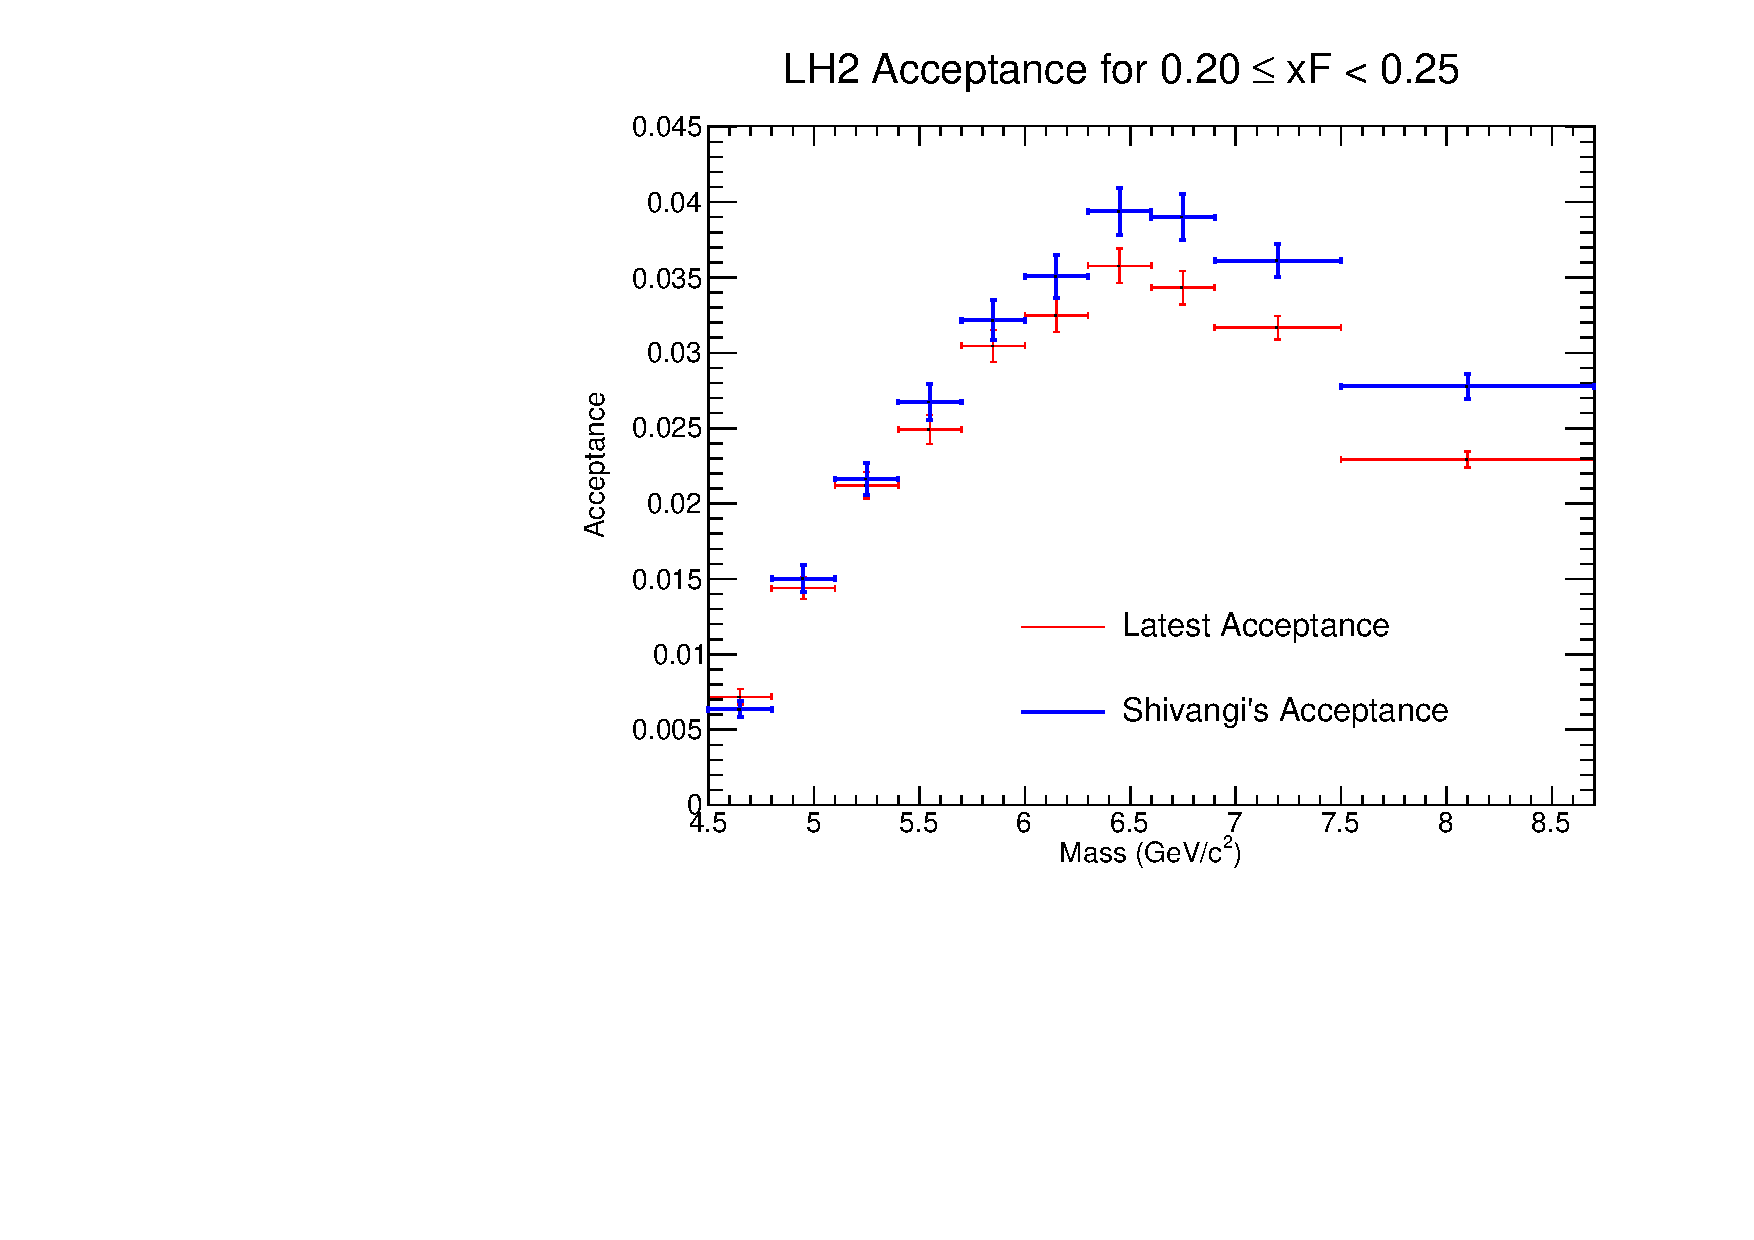
\includegraphics[width=\linewidth]{LH2_acceptance_xF_bin_4.pdf}
       \caption{Acceptance for LH2}
    \end{subfigure}
    \hfill
    \begin{subfigure}[b]{0.48\textwidth}
       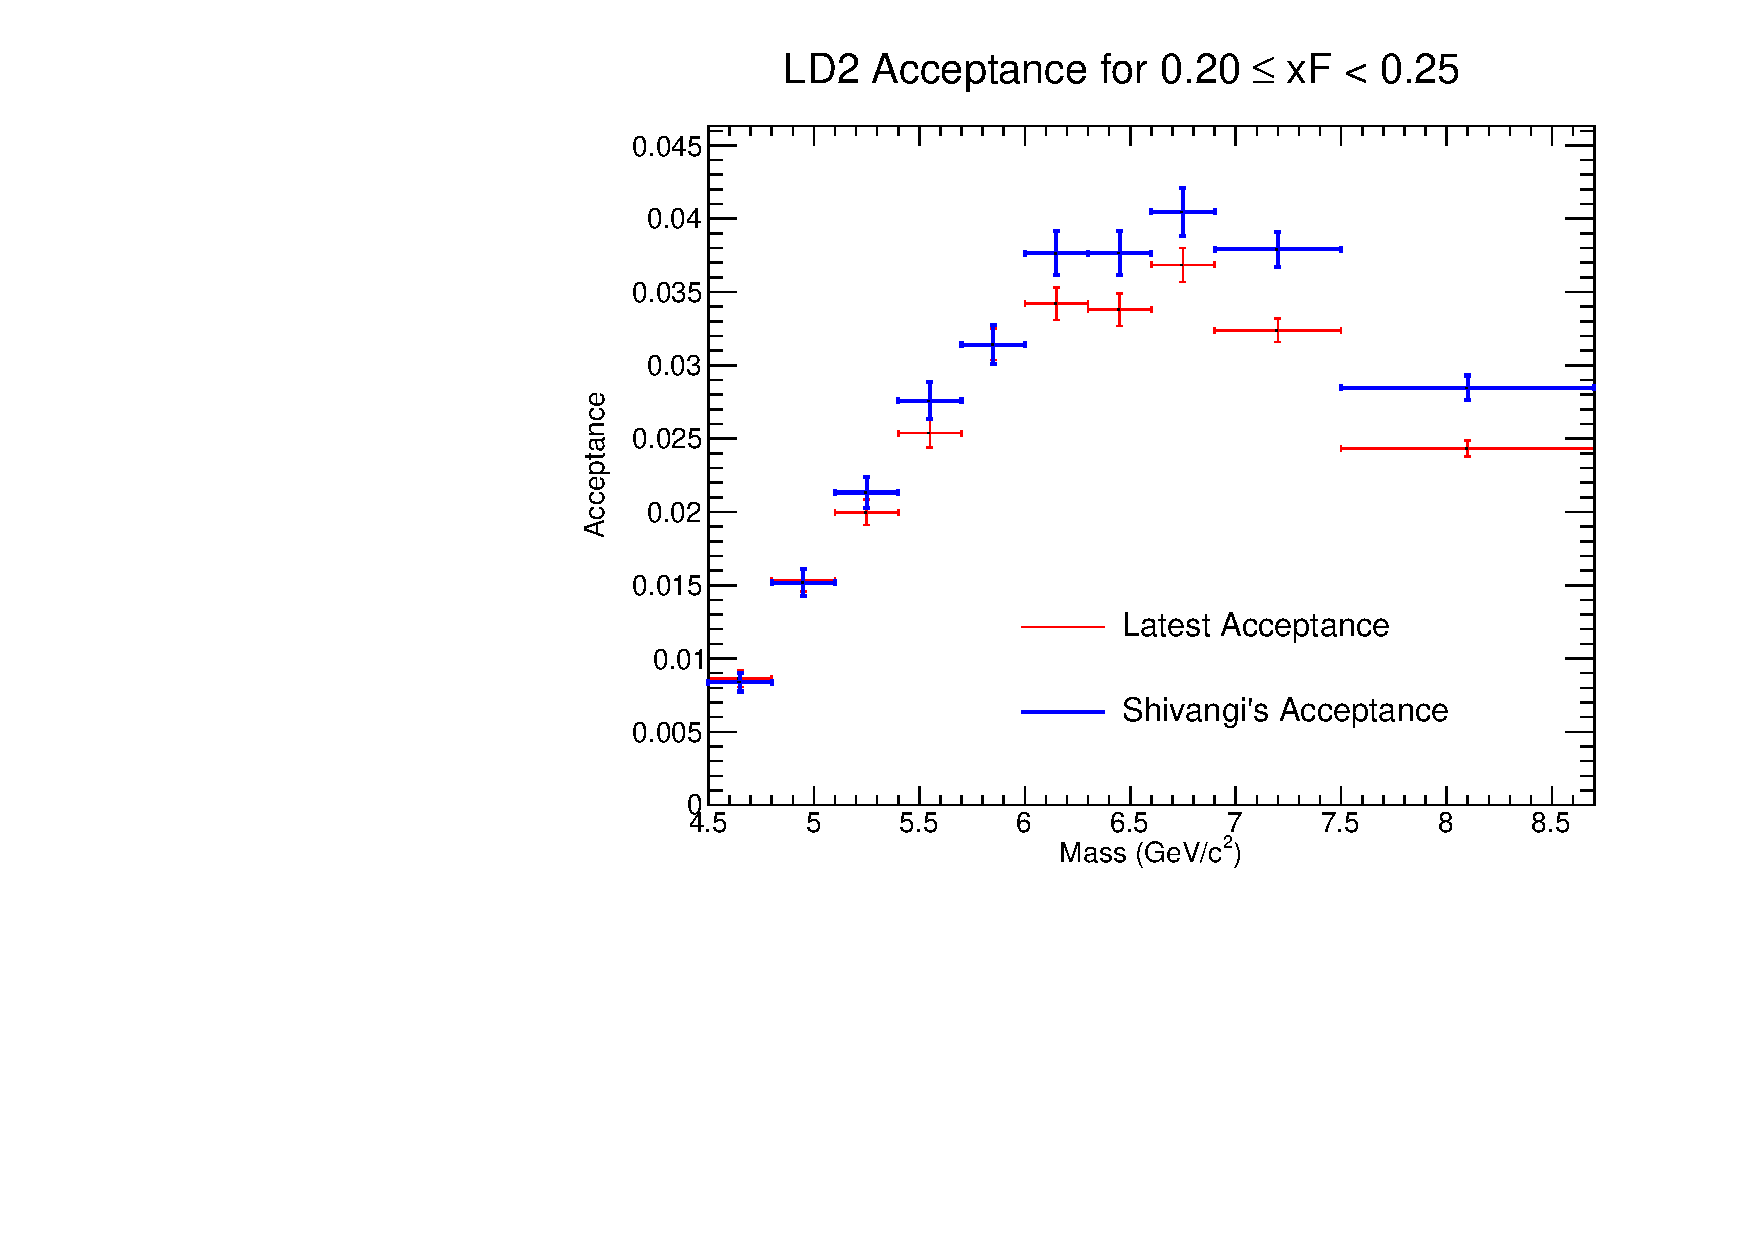
\includegraphics[width=\linewidth]{LD2_acceptance_xF_bin_4.pdf}
       \caption{Acceptance for LD2}
    \end{subfigure}

    \begin{subfigure}[b]{0.48\textwidth}
       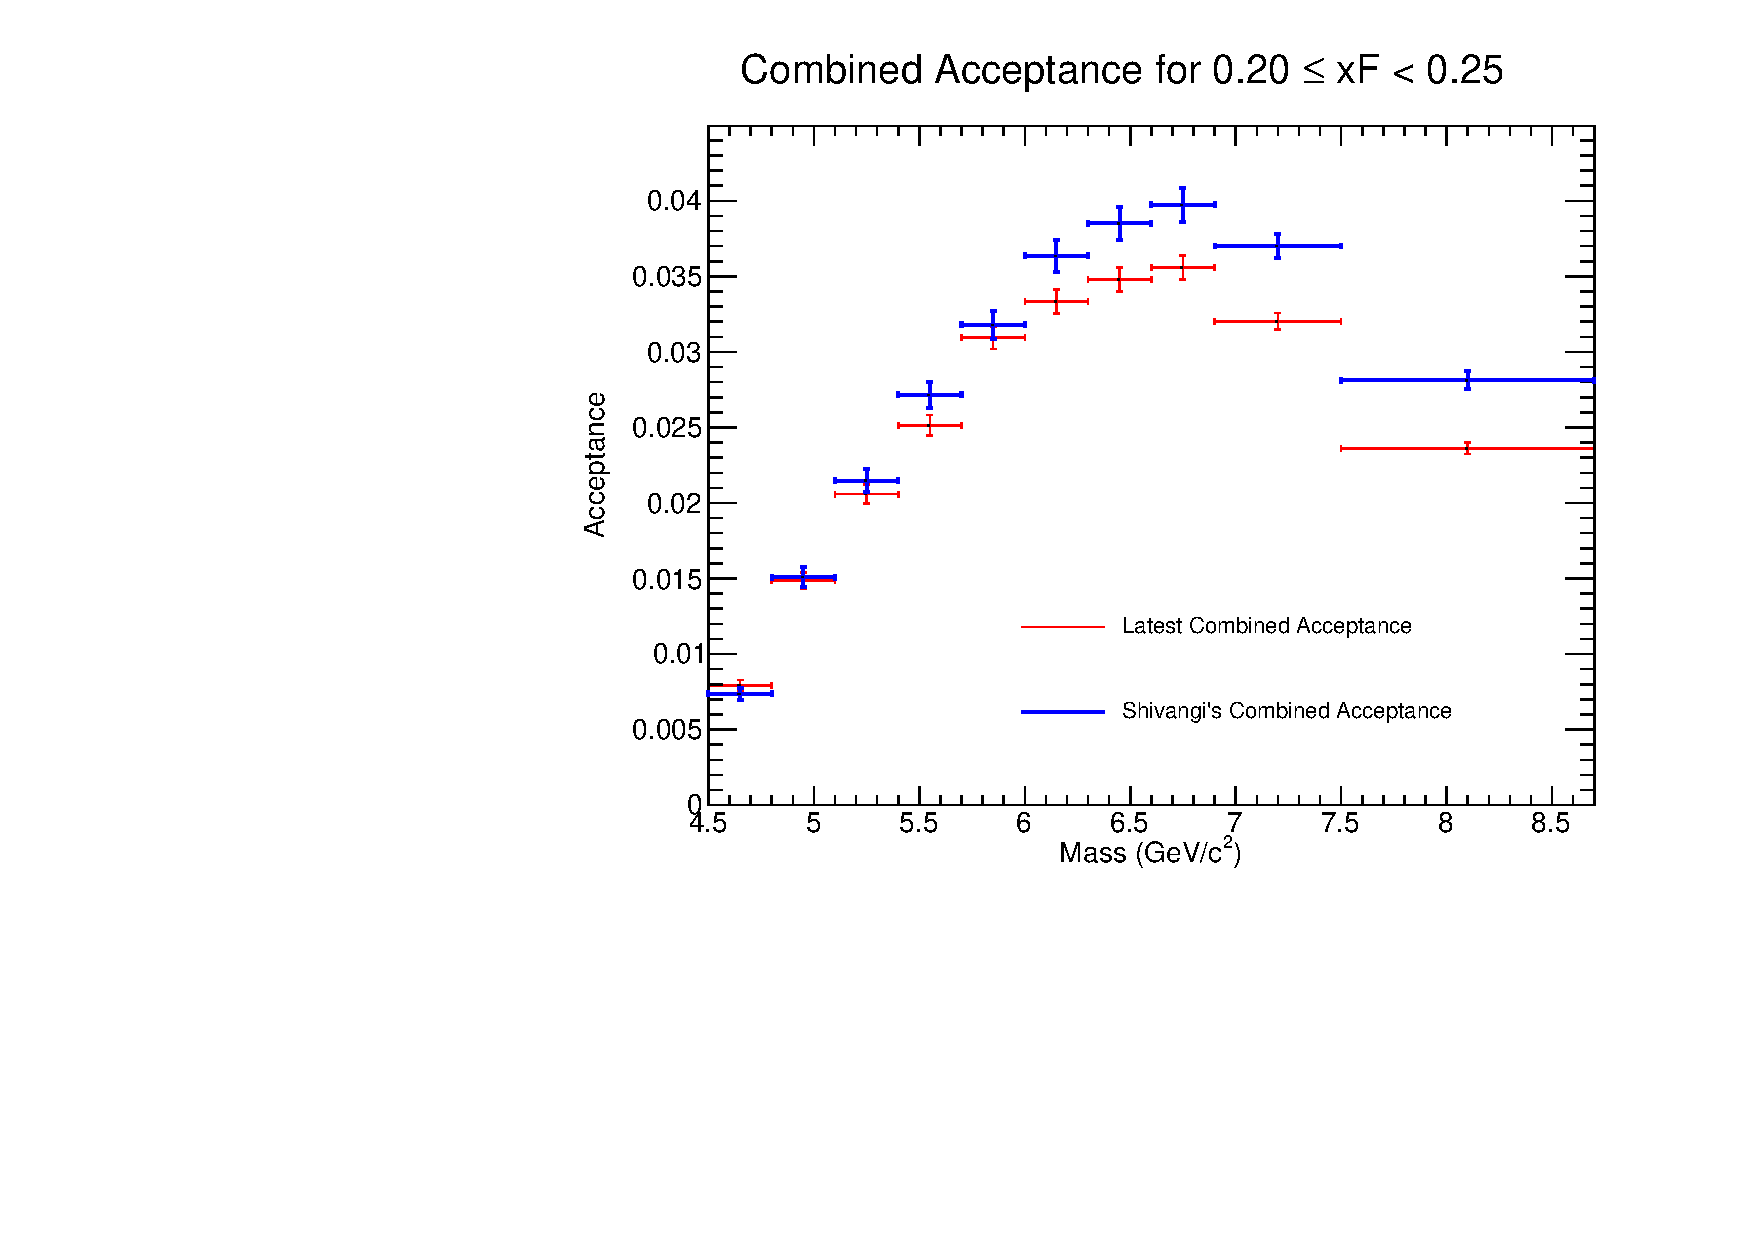
\includegraphics[width=\linewidth]{Combined_acceptance_xF_bin_4.pdf}
       \caption{Combined Acceptance}
    \end{subfigure}
    \hfill
    \begin{subfigure}[b]{0.48\textwidth}
       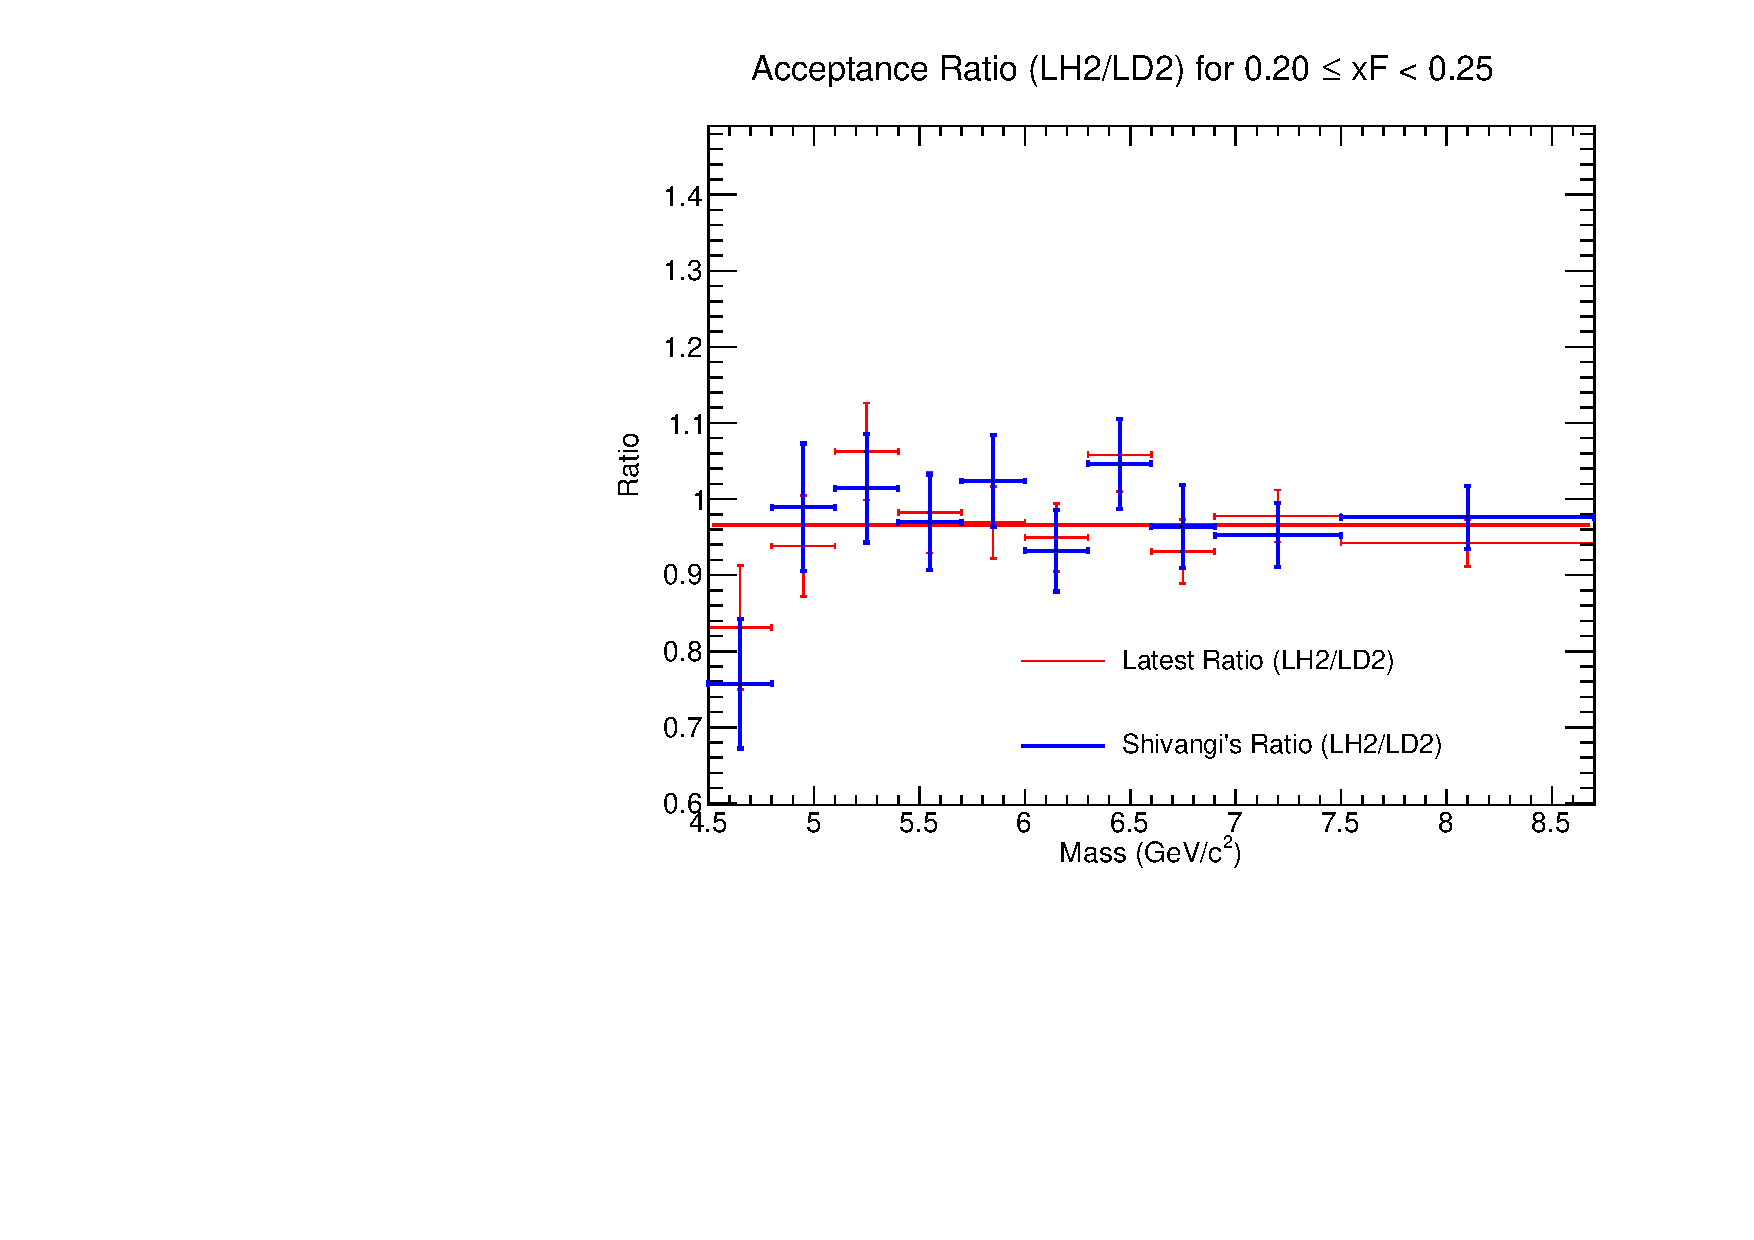
\includegraphics[width=\linewidth]{Acceptance_ratio_xF_bin_4.pdf}
       \caption{Acceptance Ratio (LH2/LD2)}
    \end{subfigure}
    \caption{Acceptance plots for $0.20 \le x_F < 0.25$.}
\end{figure}

\begin{figure}[H]
    \centering
    \begin{subfigure}[b]{0.48\textwidth}
       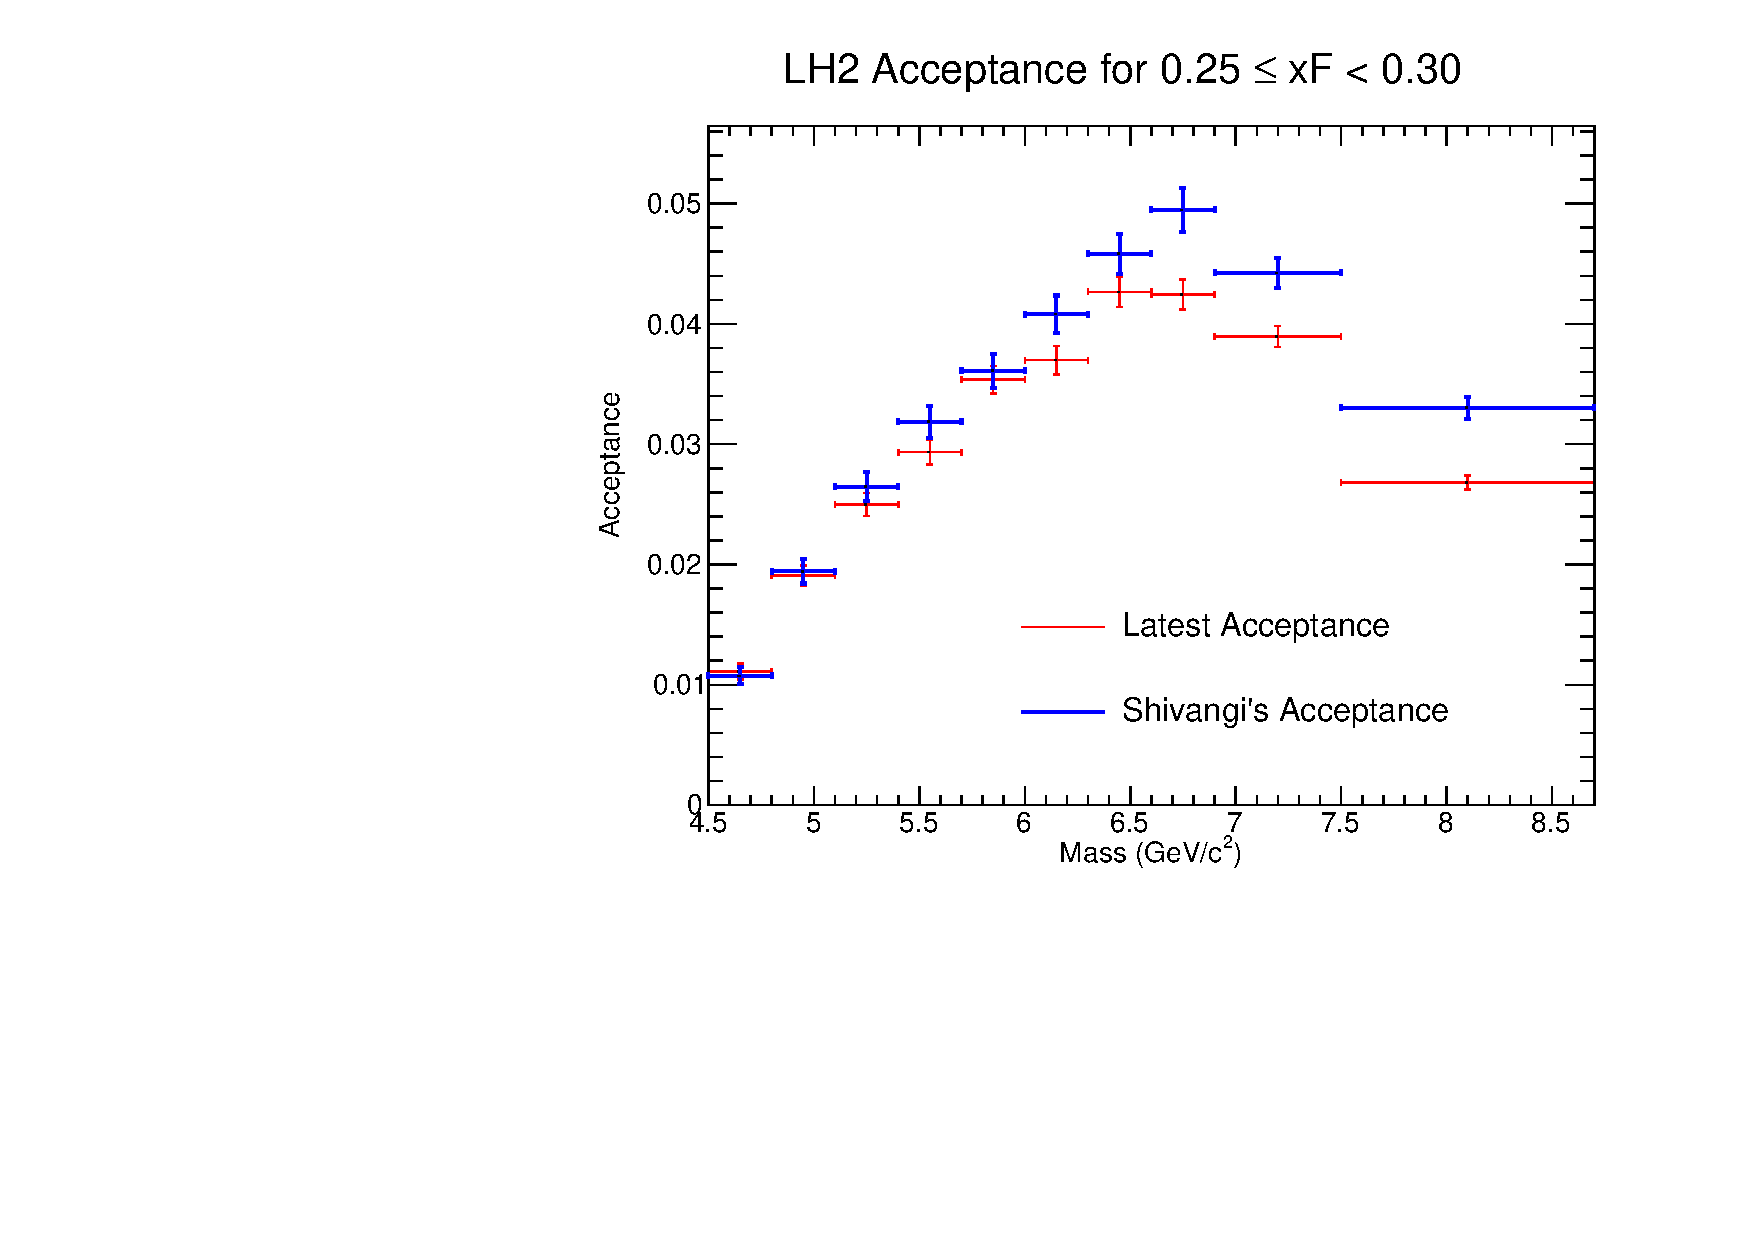
\includegraphics[width=\linewidth]{LH2_acceptance_xF_bin_5.pdf}
       \caption{Acceptance for LH2}
    \end{subfigure}
    \hfill
    \begin{subfigure}[b]{0.48\textwidth}
       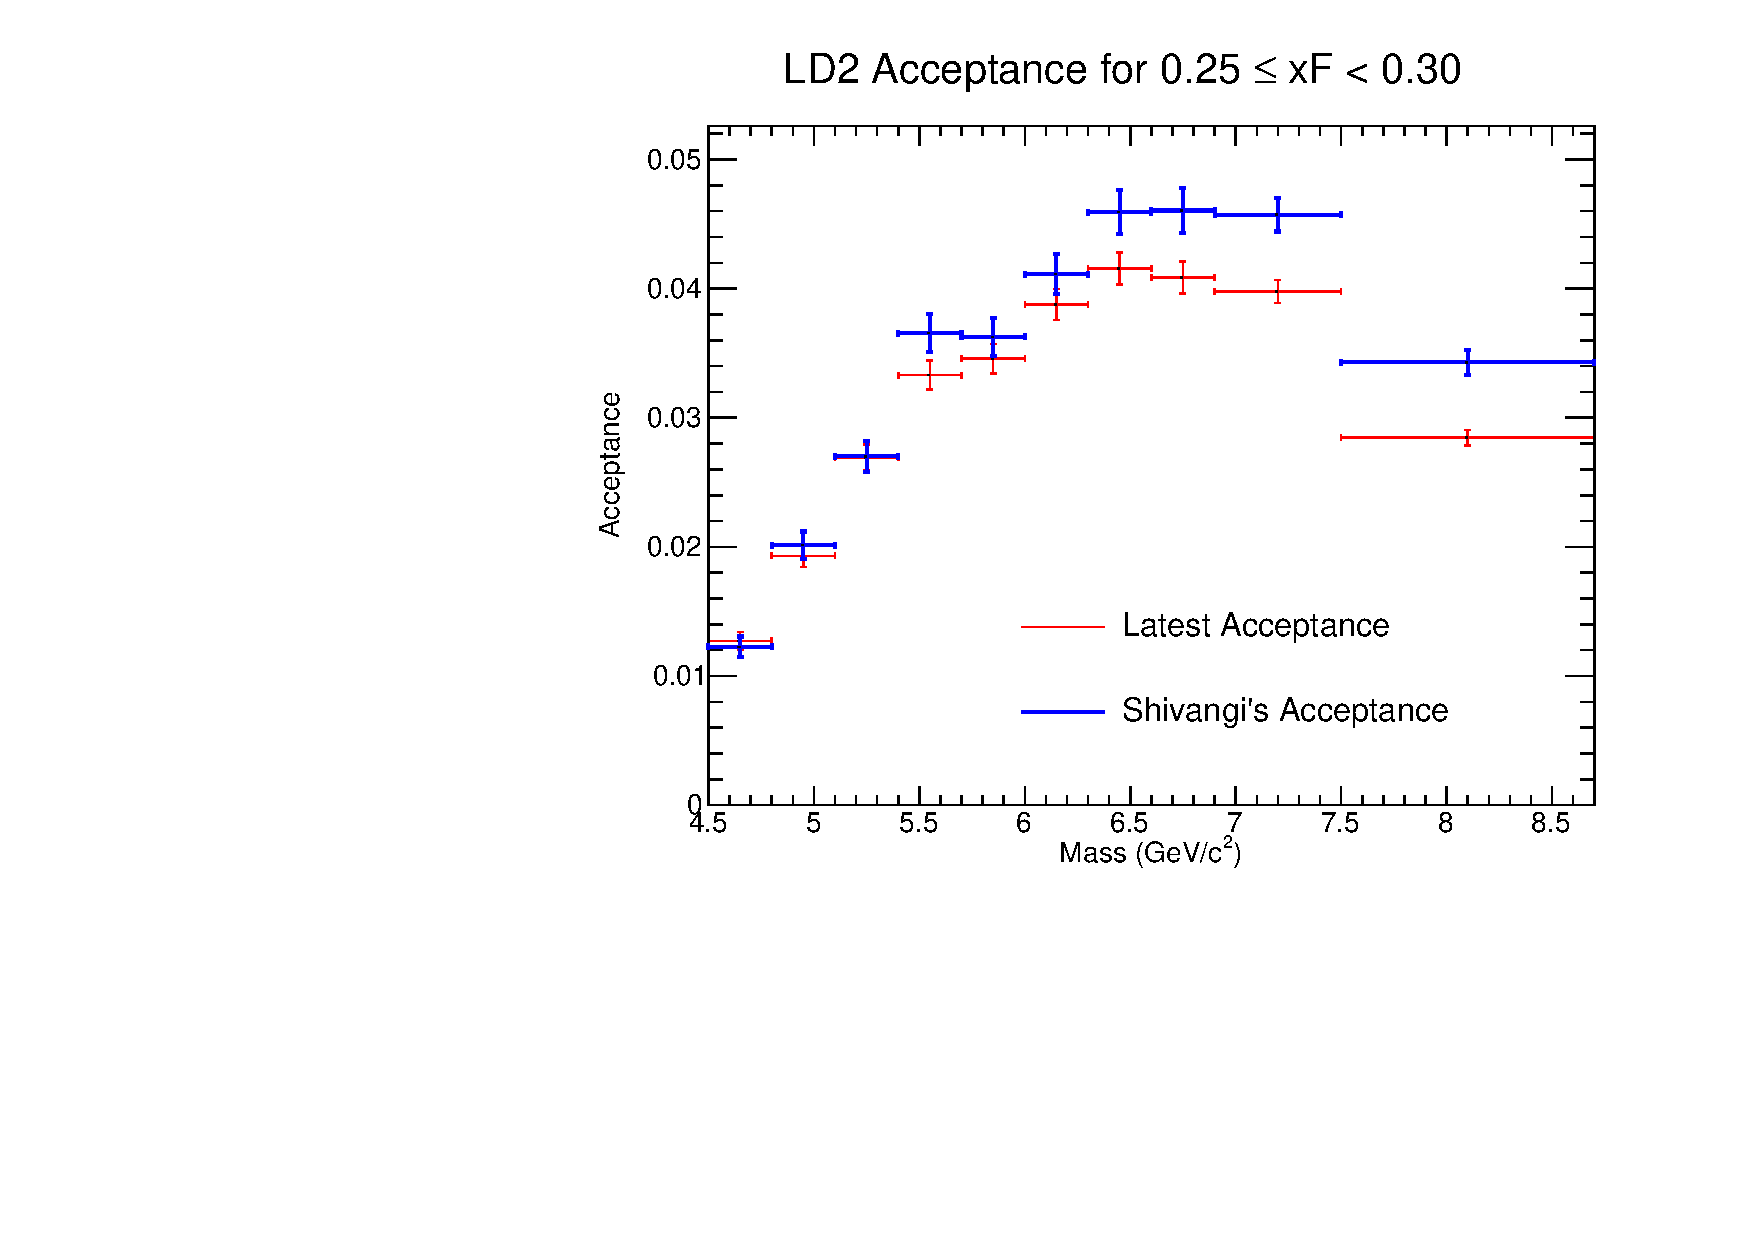
\includegraphics[width=\linewidth]{LD2_acceptance_xF_bin_5.pdf}
       \caption{Acceptance for LD2}
    \end{subfigure}

    \begin{subfigure}[b]{0.48\textwidth}
       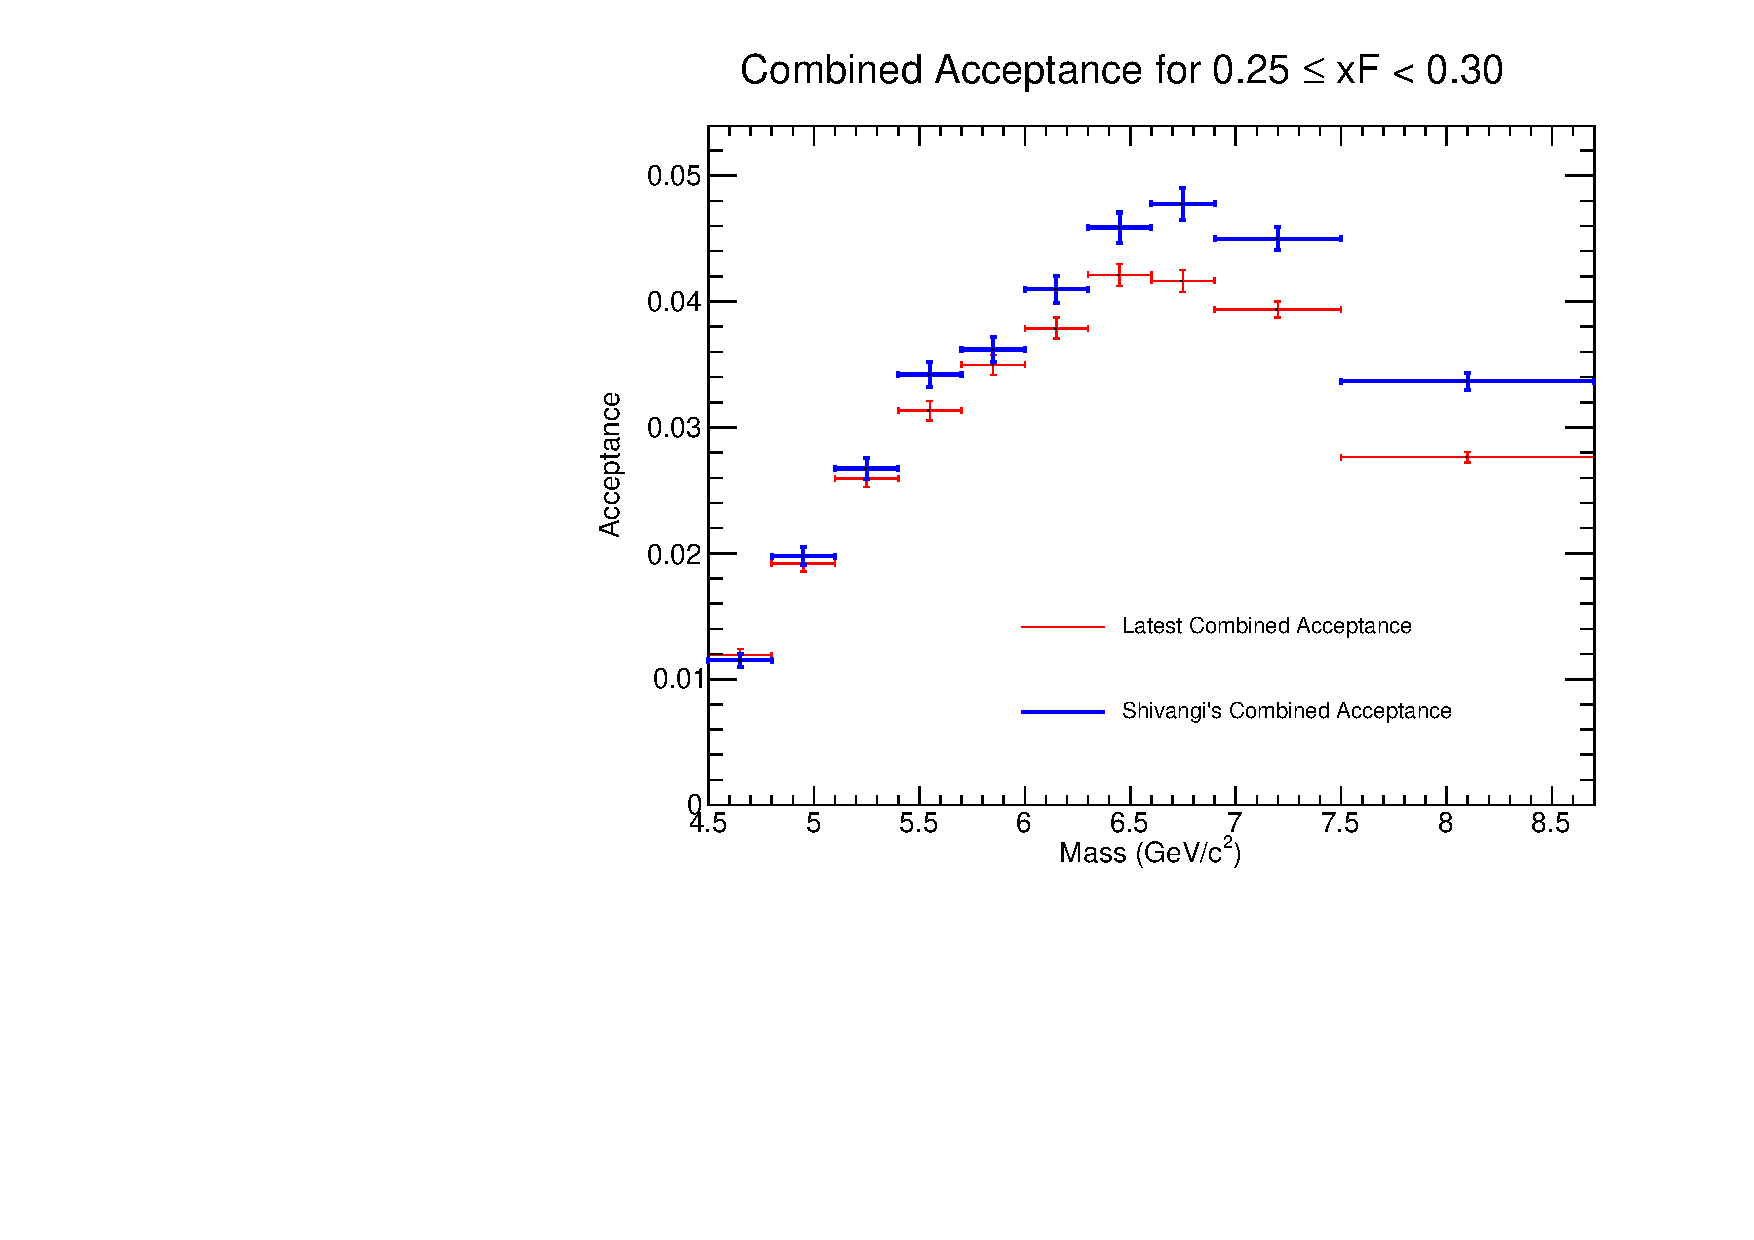
\includegraphics[width=\linewidth]{Combined_acceptance_xF_bin_5.pdf}
       \caption{Combined Acceptance}
    \end{subfigure}
    \hfill
    \begin{subfigure}[b]{0.48\textwidth}
       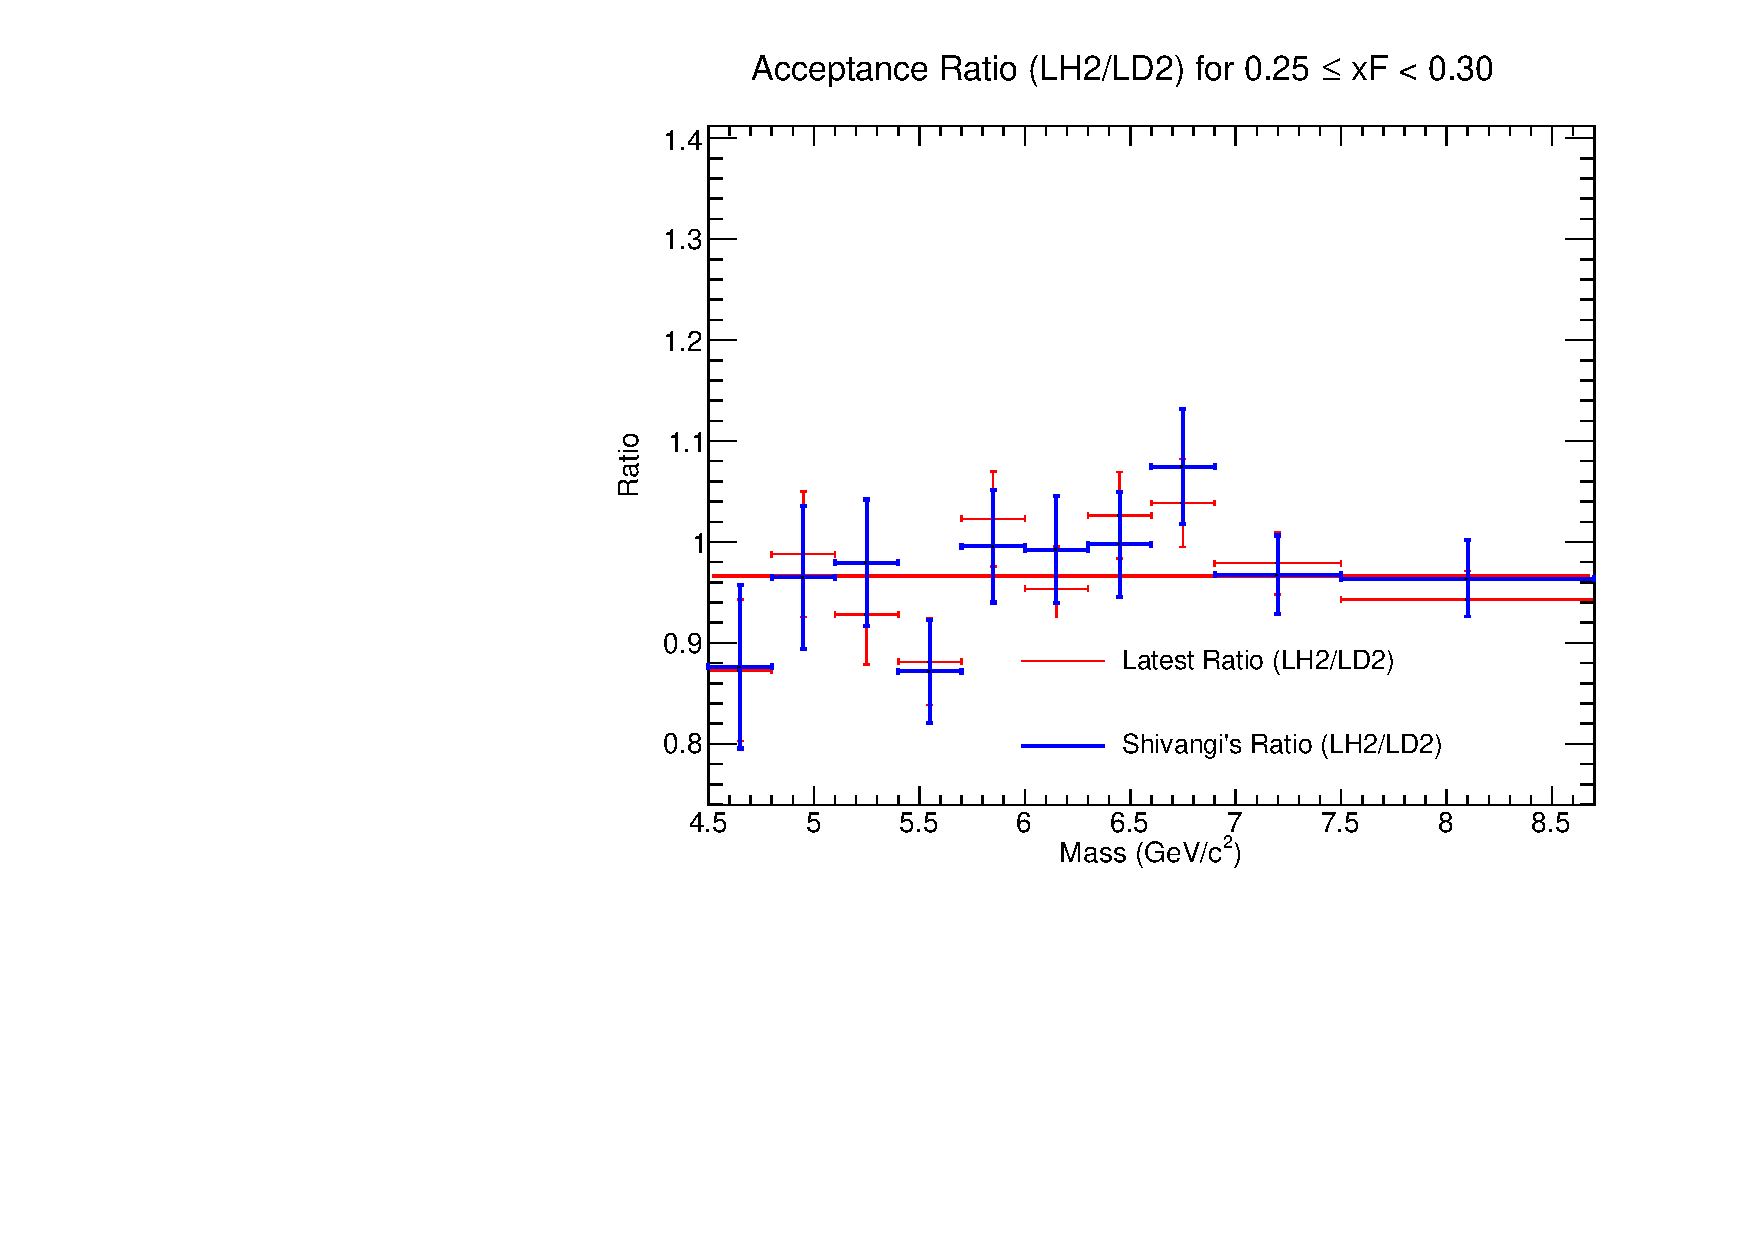
\includegraphics[width=\linewidth]{Acceptance_ratio_xF_bin_5.pdf}
       \caption{Acceptance Ratio (LH2/LD2)}
    \end{subfigure}
    \caption{Acceptance plots for $0.25 \le x_F < 0.30$.}
\end{figure}

\begin{figure}[H]
    \centering
    \begin{subfigure}[b]{0.48\textwidth}
       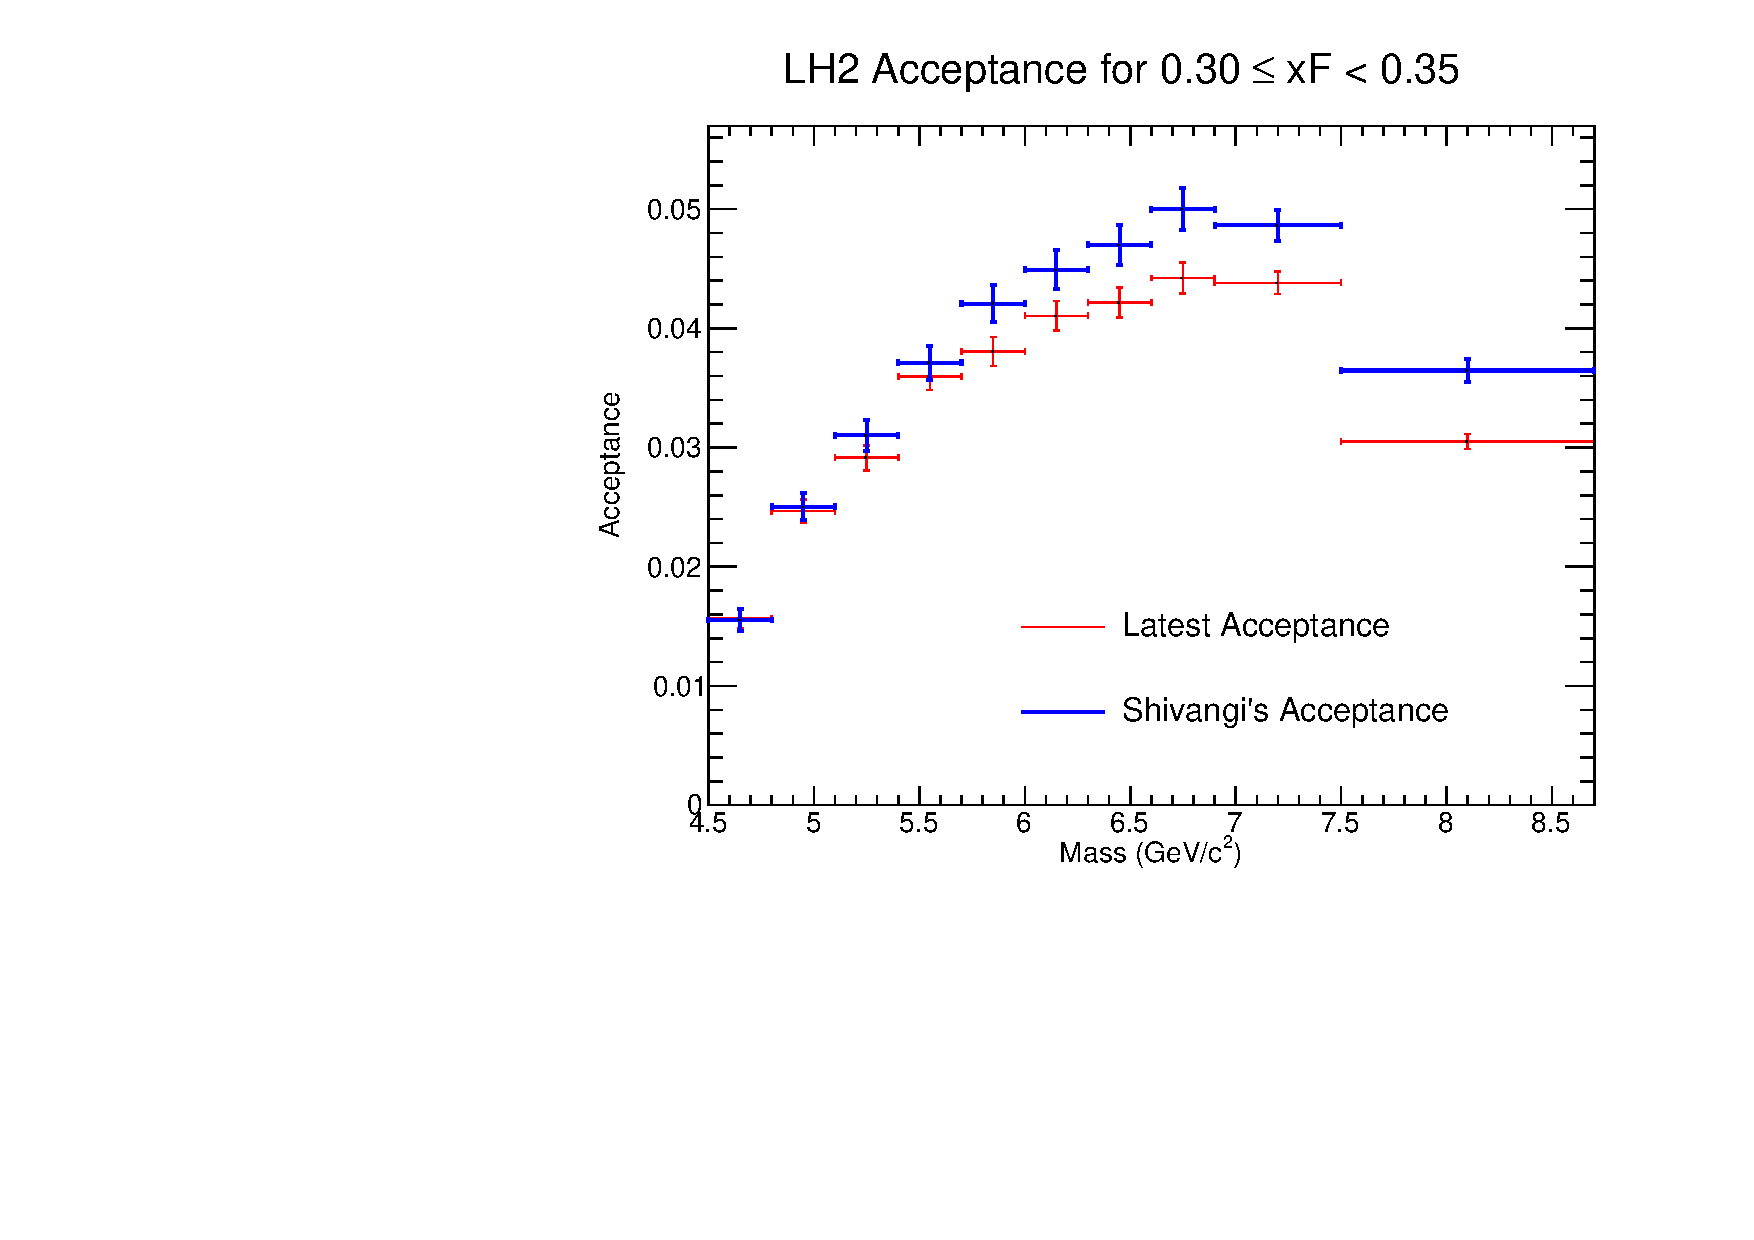
\includegraphics[width=\linewidth]{LH2_acceptance_xF_bin_6.pdf}
       \caption{Acceptance for LH2}
    \end{subfigure}
    \hfill
    \begin{subfigure}[b]{0.48\textwidth}
       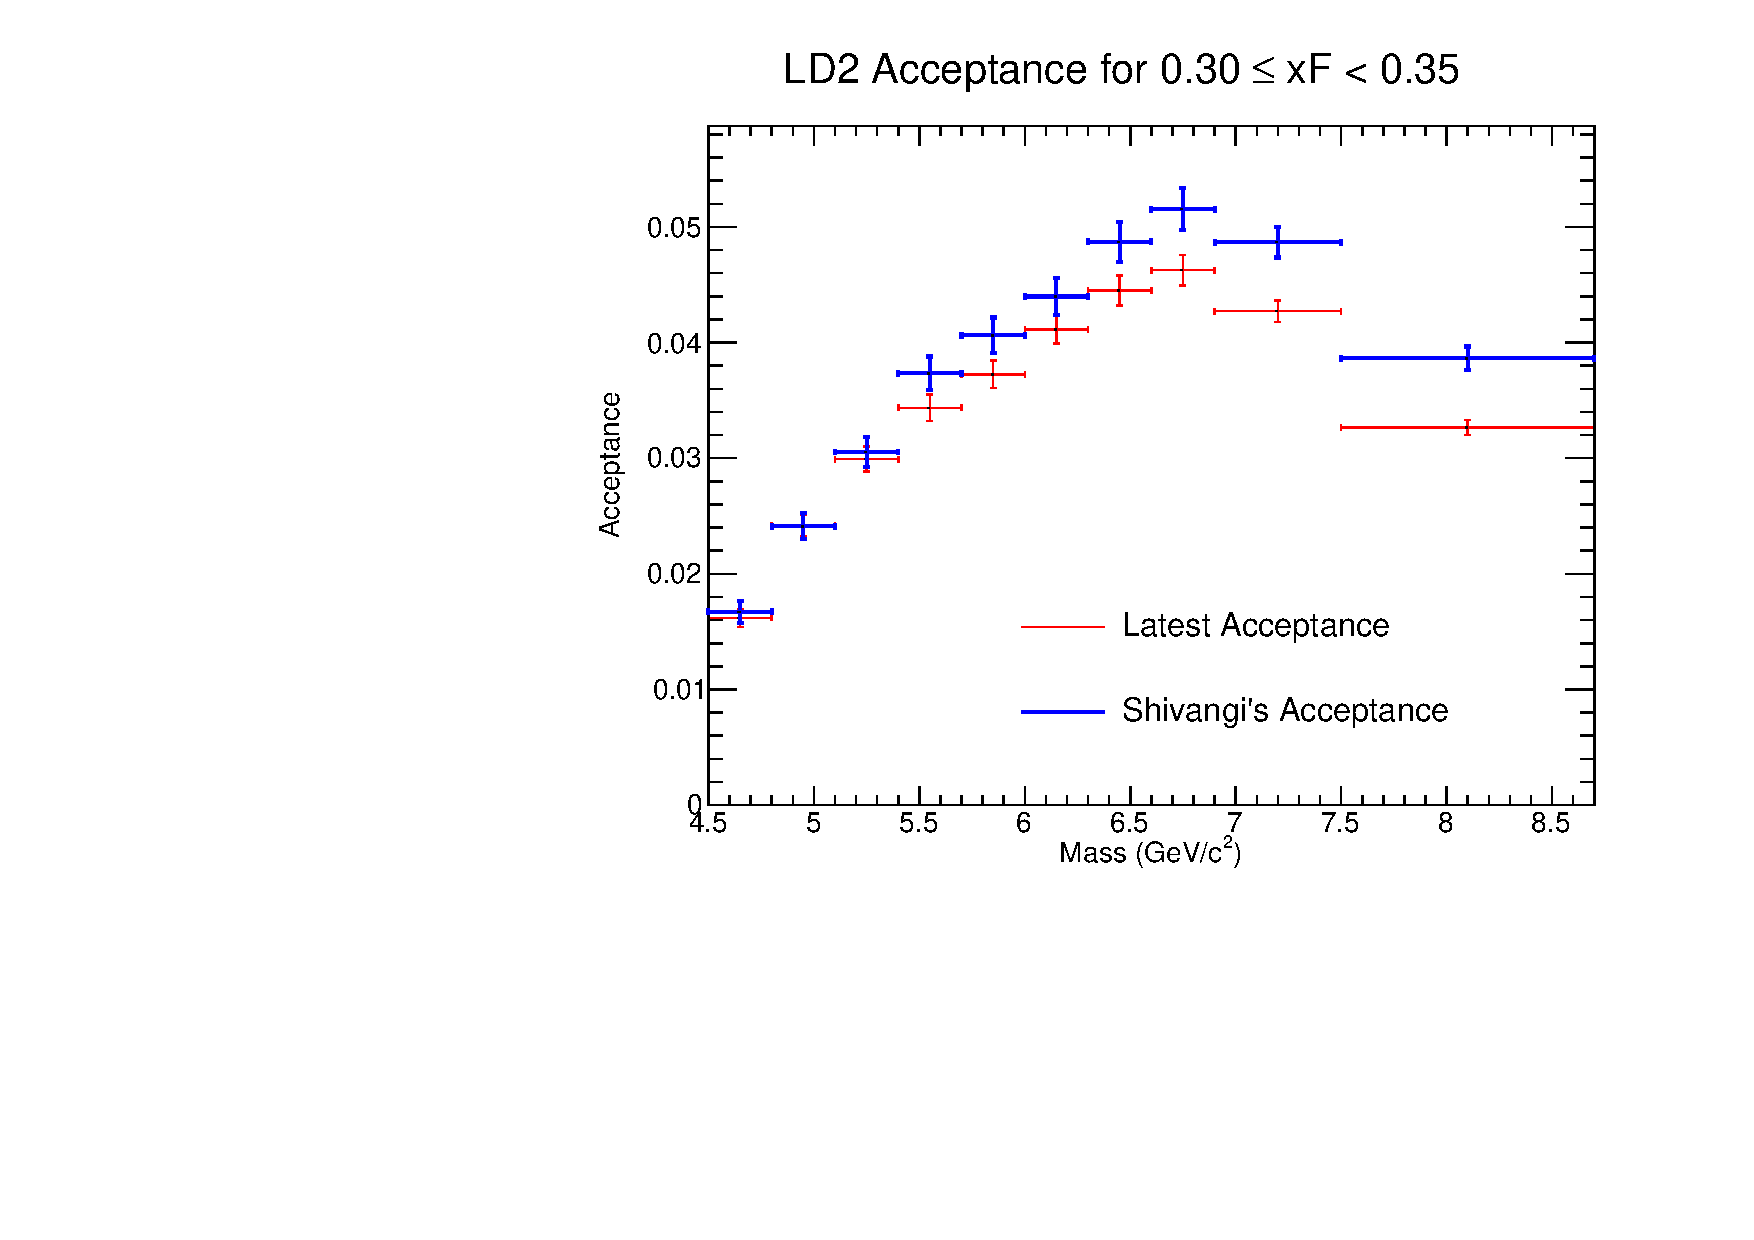
\includegraphics[width=\linewidth]{LD2_acceptance_xF_bin_6.pdf}
       \caption{Acceptance for LD2}
    \end{subfigure}

    \begin{subfigure}[b]{0.48\textwidth}
       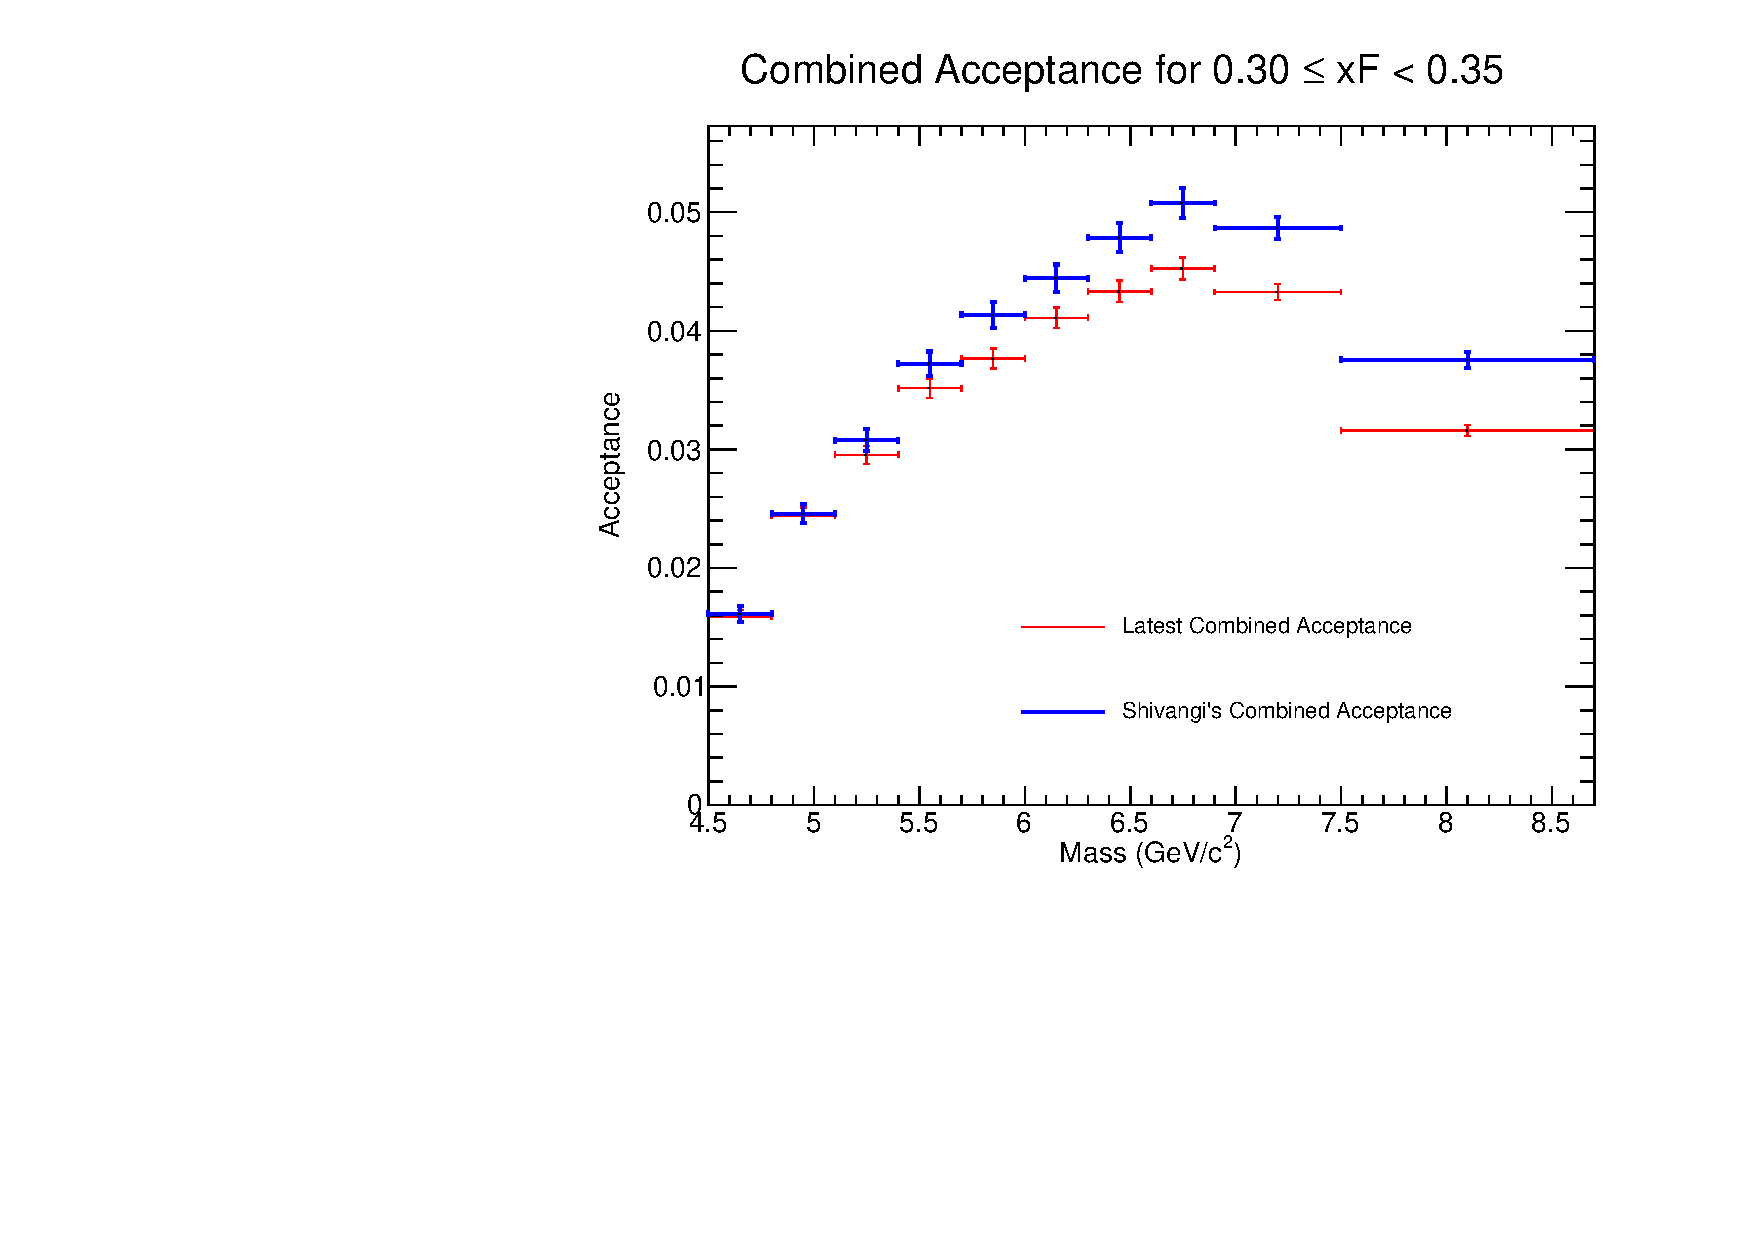
\includegraphics[width=\linewidth]{Combined_acceptance_xF_bin_6.pdf}
       \caption{Combined Acceptance}
    \end{subfigure}
    \hfill
    \begin{subfigure}[b]{0.48\textwidth}
       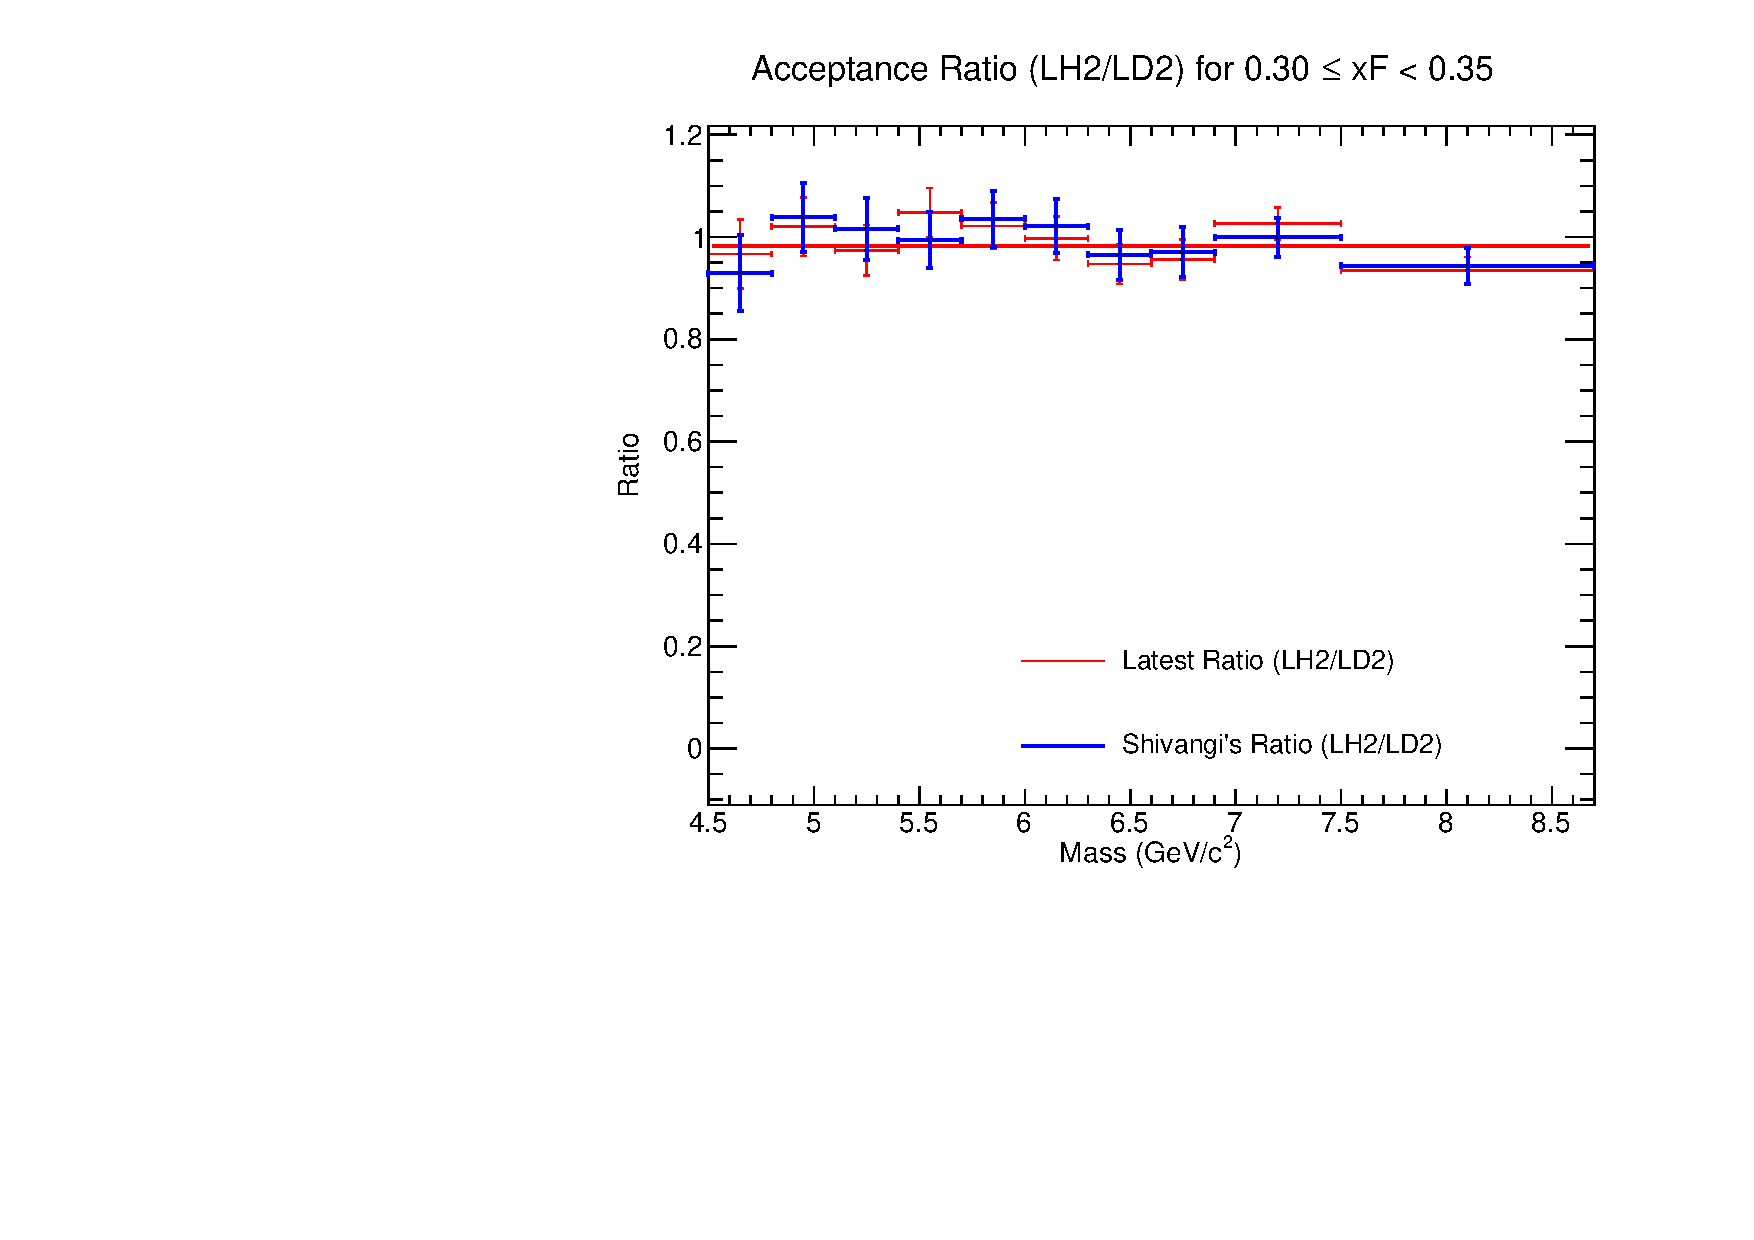
\includegraphics[width=\linewidth]{Acceptance_ratio_xF_bin_6.pdf}
       \caption{Acceptance Ratio (LH2/LD2)}
    \end{subfigure}
    \caption{Acceptance plots for $0.30 \le x_F < 0.35$.}
\end{figure}

\begin{figure}[H]
    \centering
    \begin{subfigure}[b]{0.48\textwidth}
       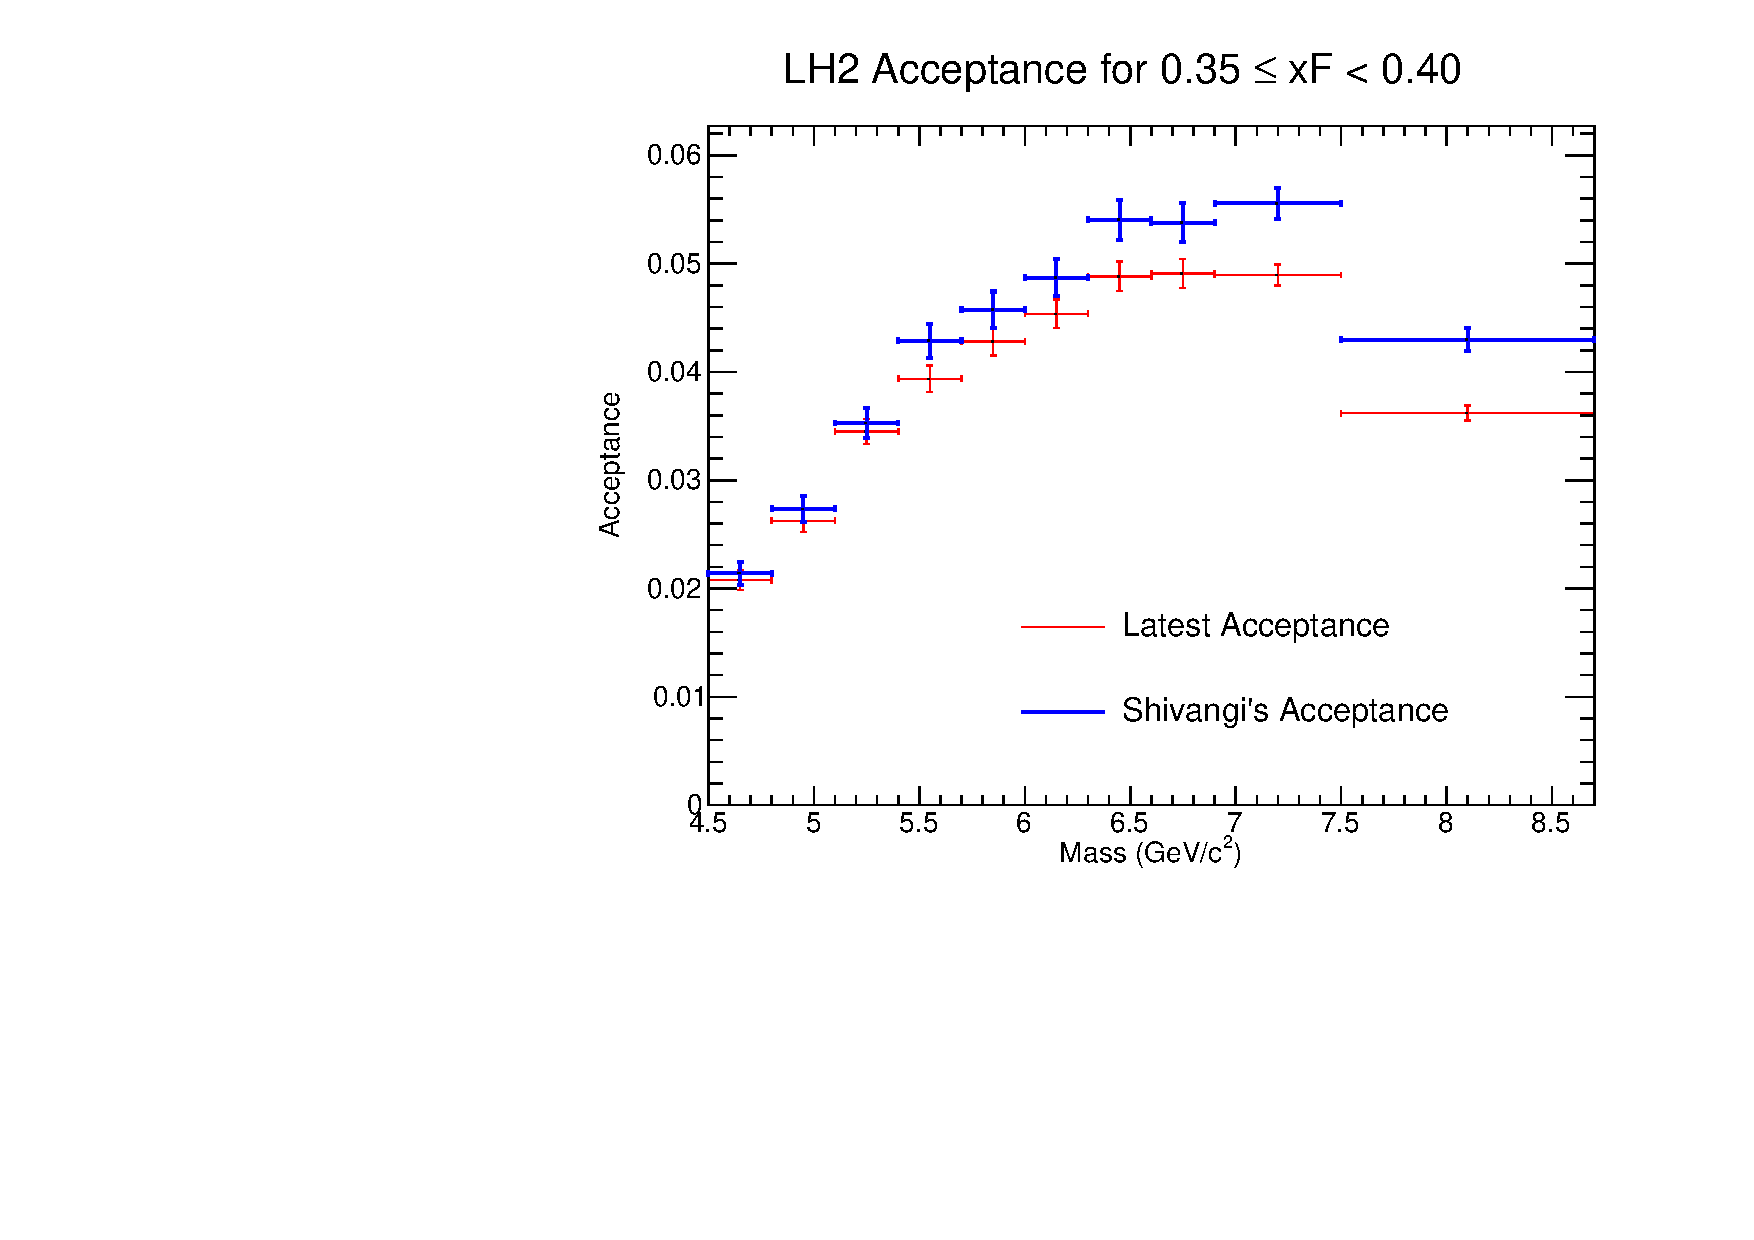
\includegraphics[width=\linewidth]{LH2_acceptance_xF_bin_7.pdf}
       \caption{Acceptance for LH2}
    \end{subfigure}
    \hfill
    \begin{subfigure}[b]{0.48\textwidth}
       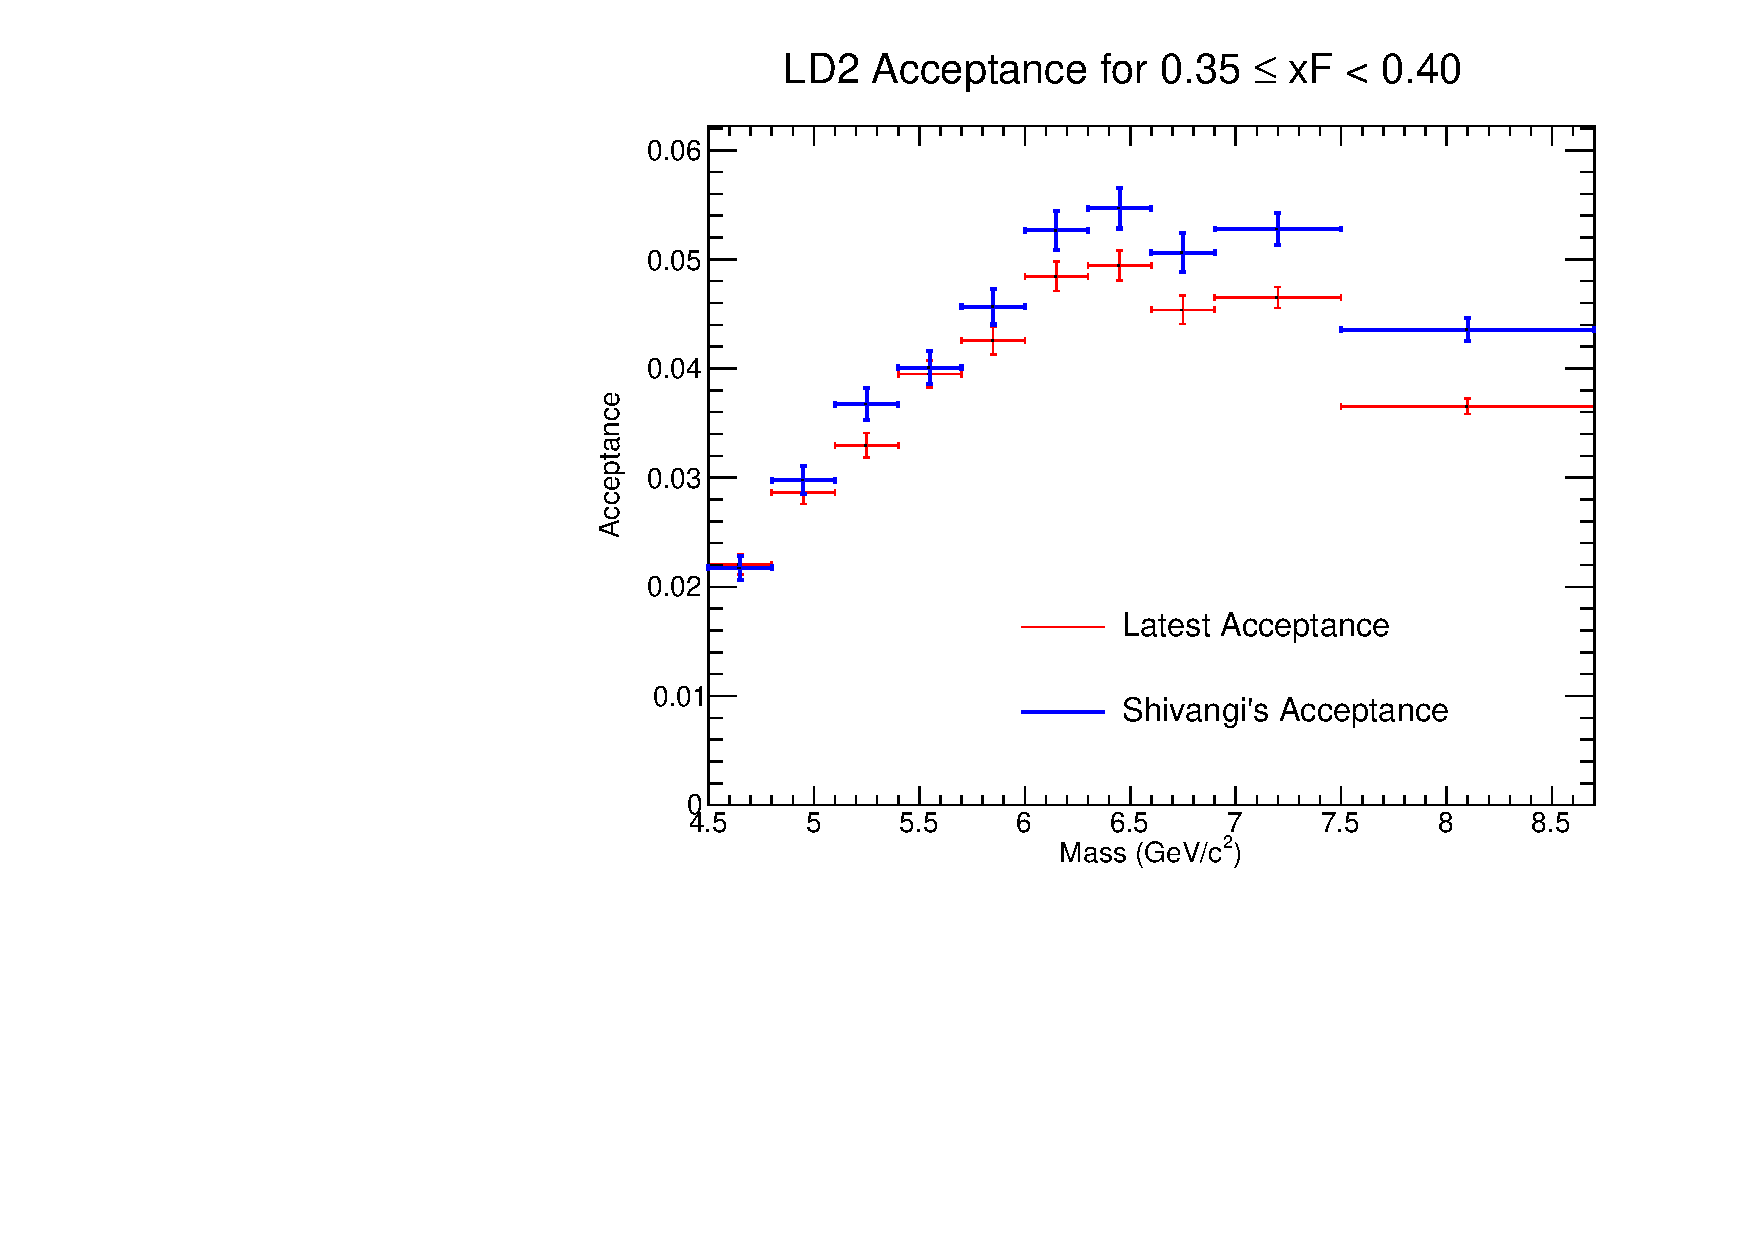
\includegraphics[width=\linewidth]{LD2_acceptance_xF_bin_7.pdf}
       \caption{Acceptance for LD2}
    \end{subfigure}

    \begin{subfigure}[b]{0.48\textwidth}
       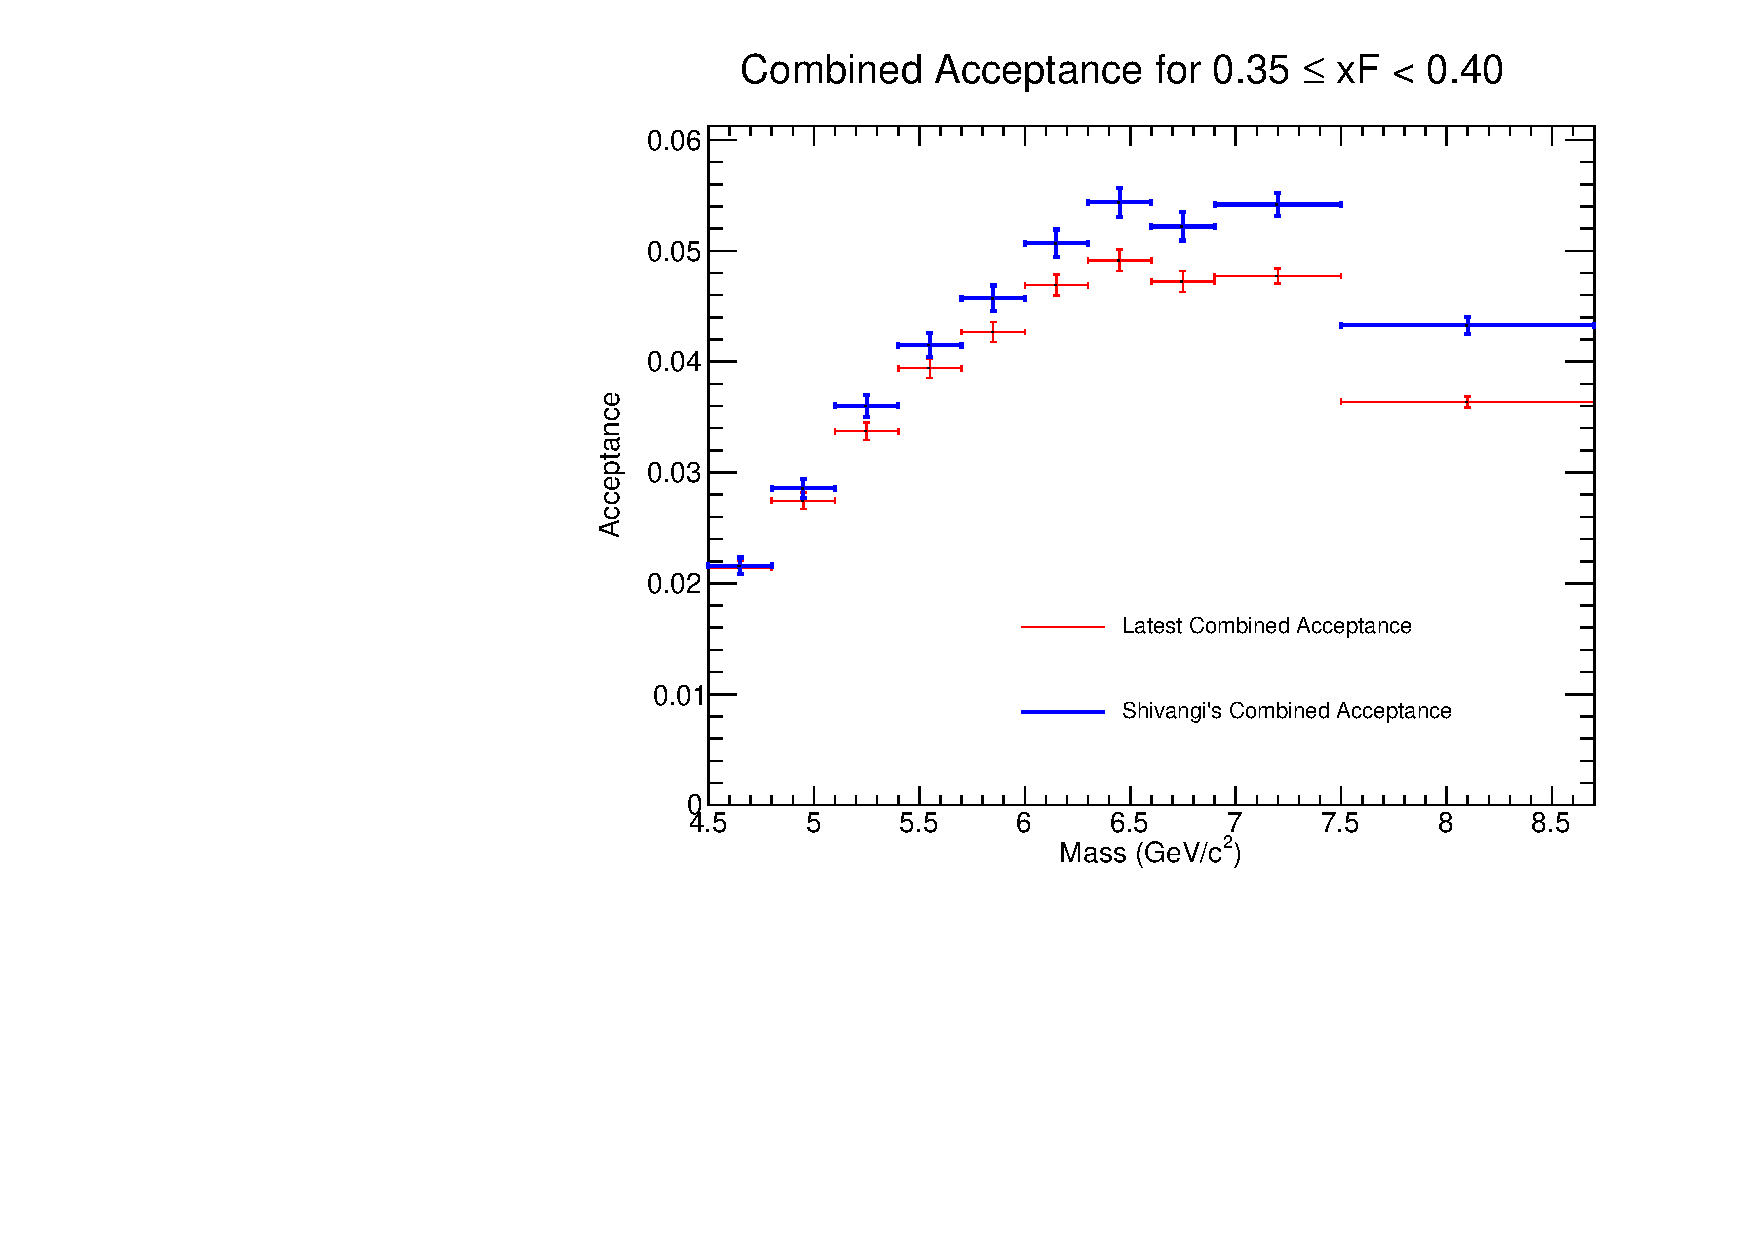
\includegraphics[width=\linewidth]{Combined_acceptance_xF_bin_7.pdf}
       \caption{Combined Acceptance}
    \end{subfigure}
    \hfill
    \begin{subfigure}[b]{0.48\textwidth}
       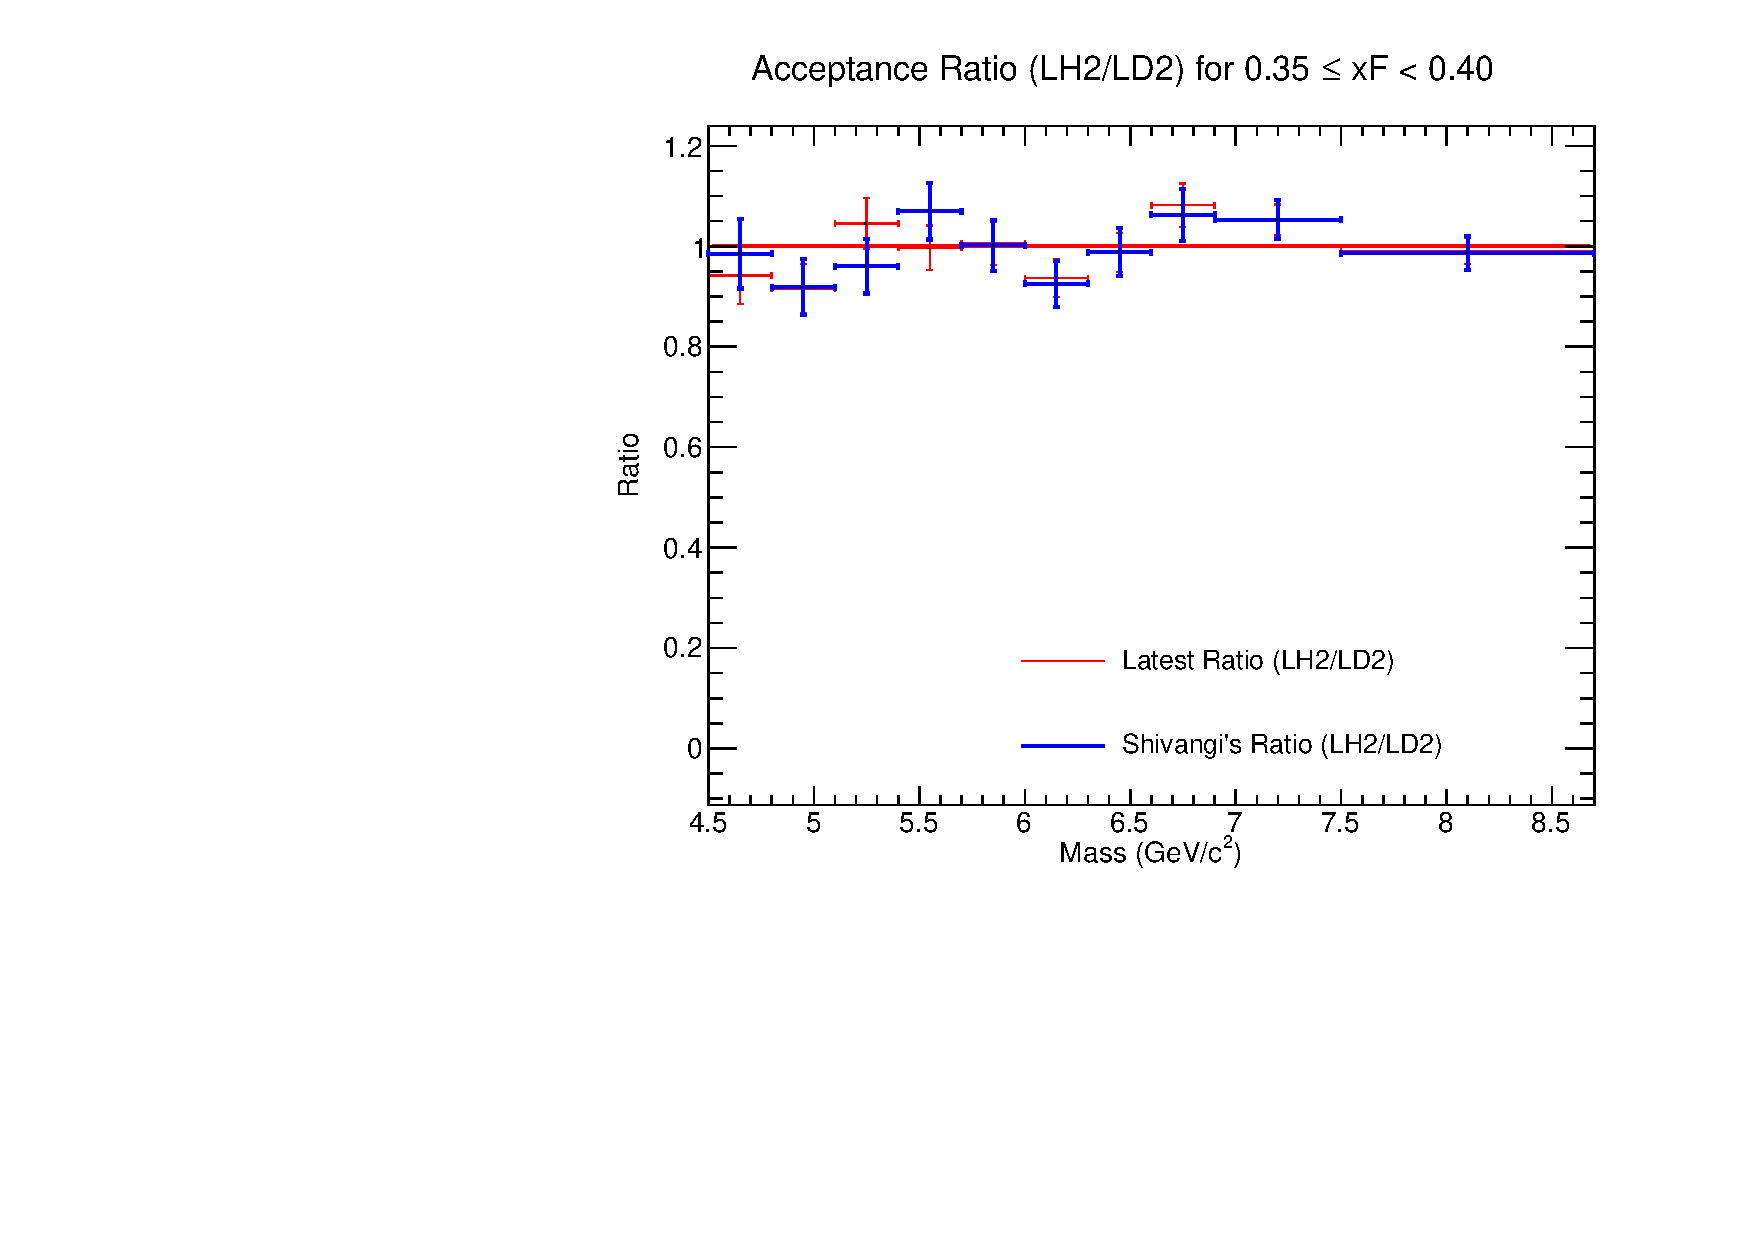
\includegraphics[width=\linewidth]{Acceptance_ratio_xF_bin_7.pdf}
       \caption{Acceptance Ratio (LH2/LD2)}
    \end{subfigure}
    \caption{Acceptance plots for $0.35 \le x_F < 0.40$.}
\end{figure}

\begin{figure}[H]
    \centering
    \begin{subfigure}[b]{0.48\textwidth}
       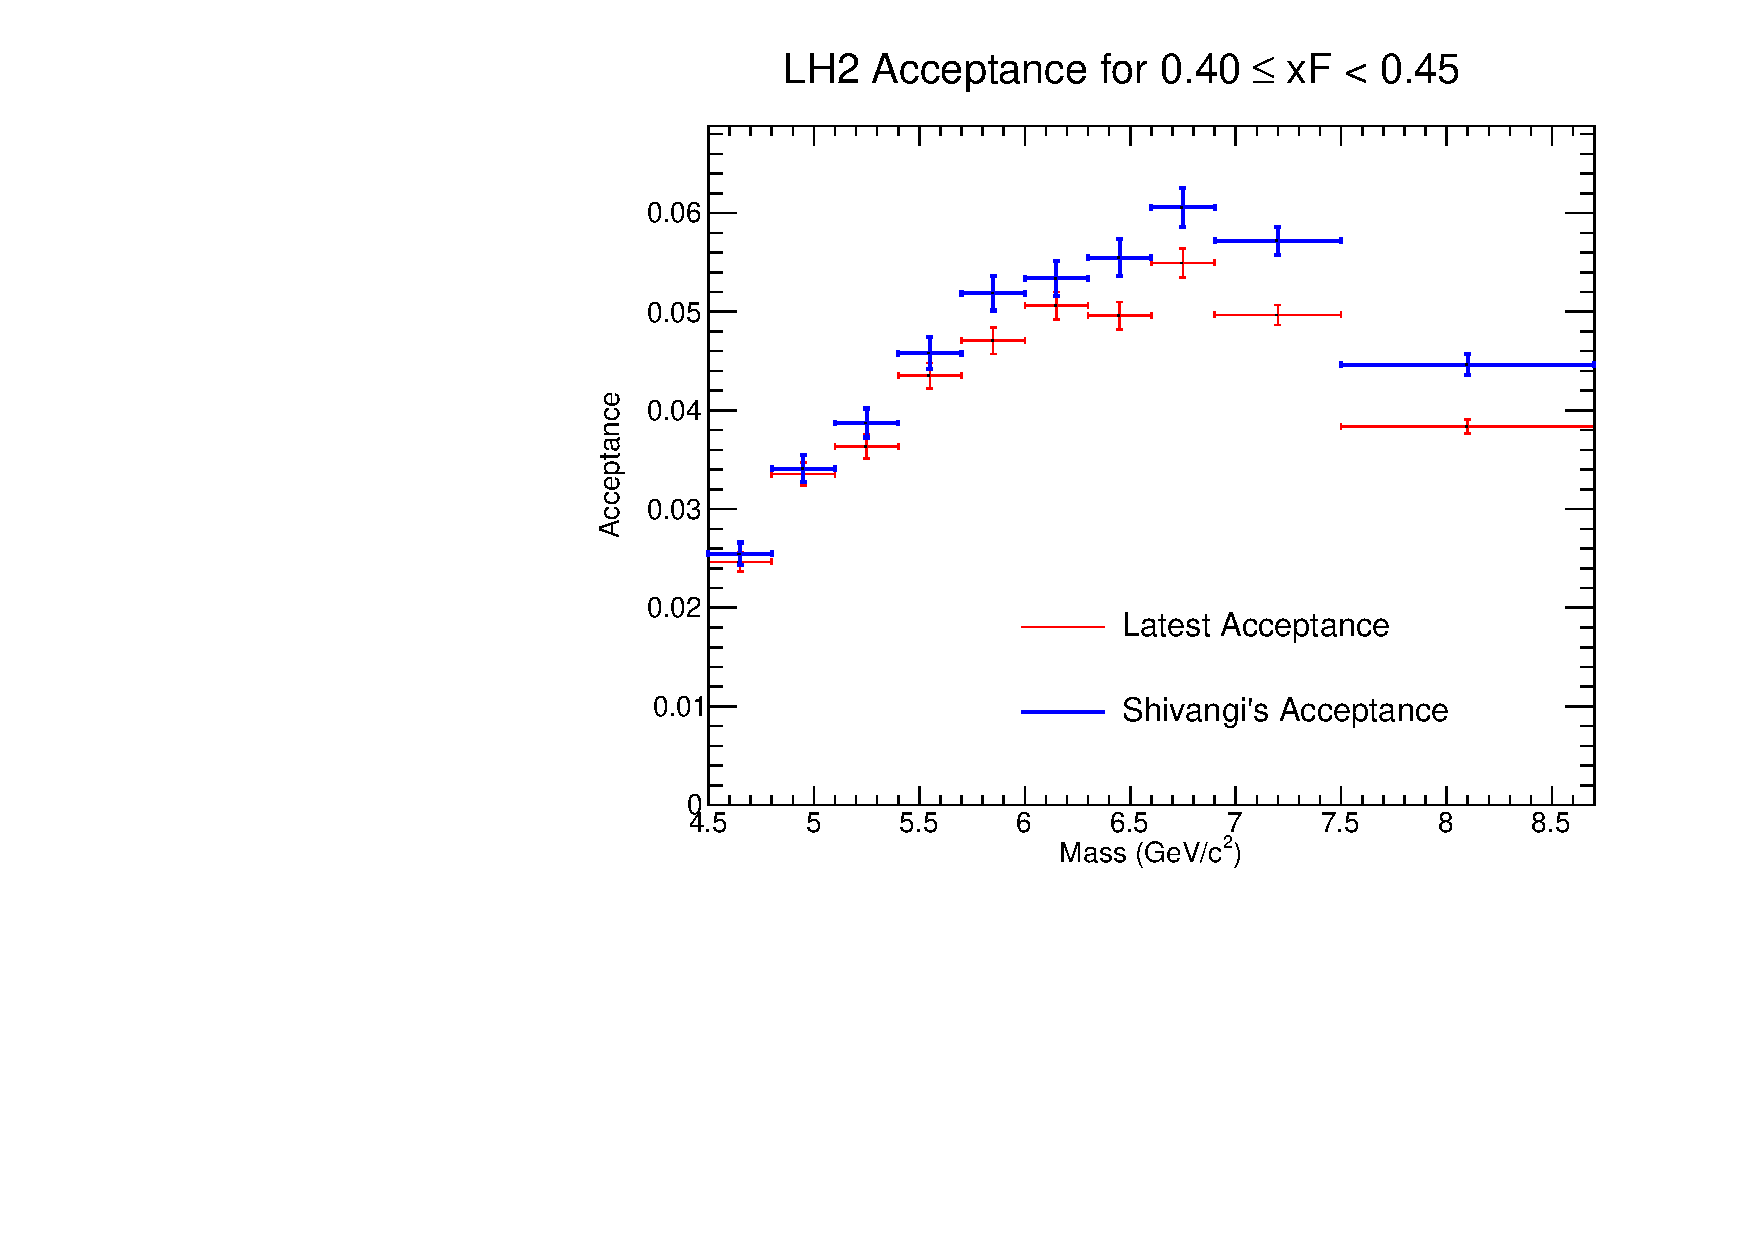
\includegraphics[width=\linewidth]{LH2_acceptance_xF_bin_8.pdf}
       \caption{Acceptance for LH2}
    \end{subfigure}
    \hfill
    \begin{subfigure}[b]{0.48\textwidth}
       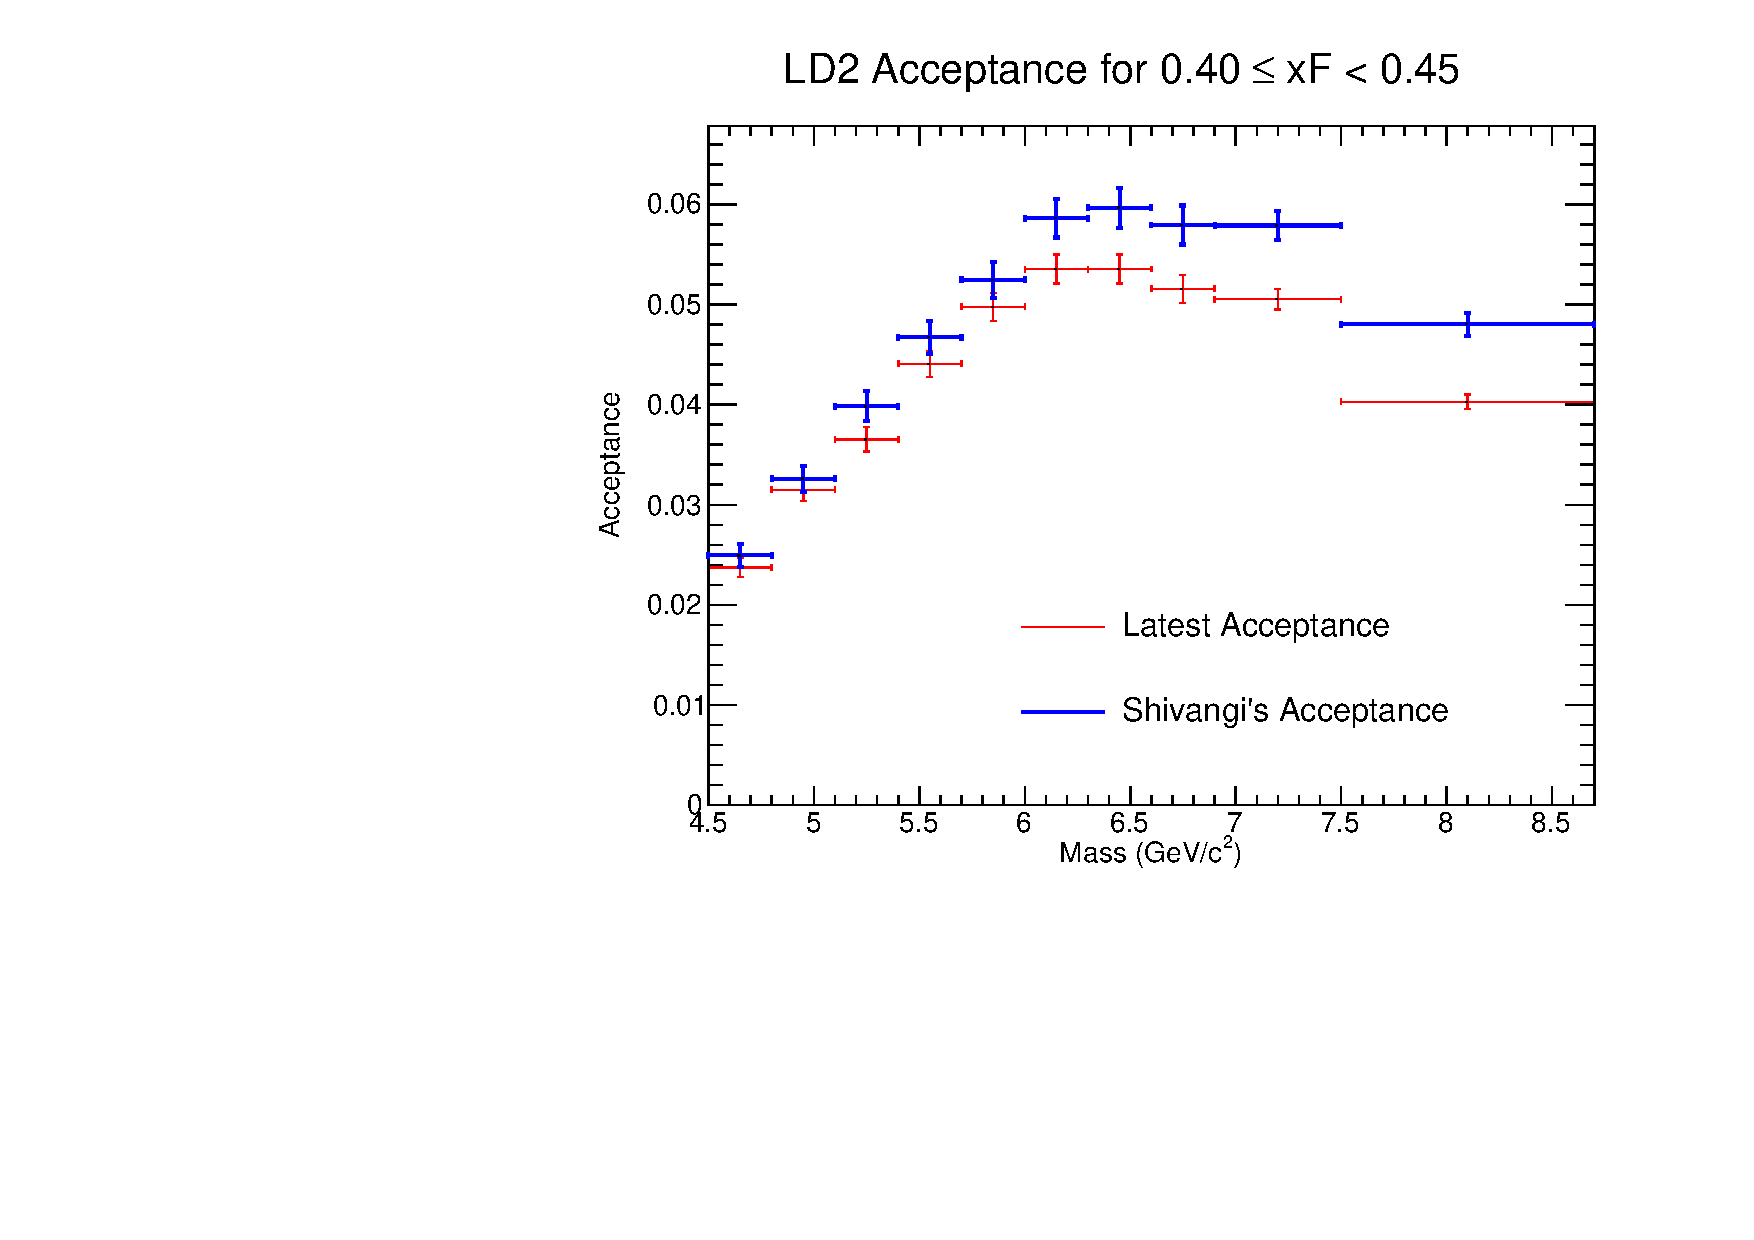
\includegraphics[width=\linewidth]{LD2_acceptance_xF_bin_8.pdf}
       \caption{Acceptance for LD2}
    \end{subfigure}

    \begin{subfigure}[b]{0.48\textwidth}
       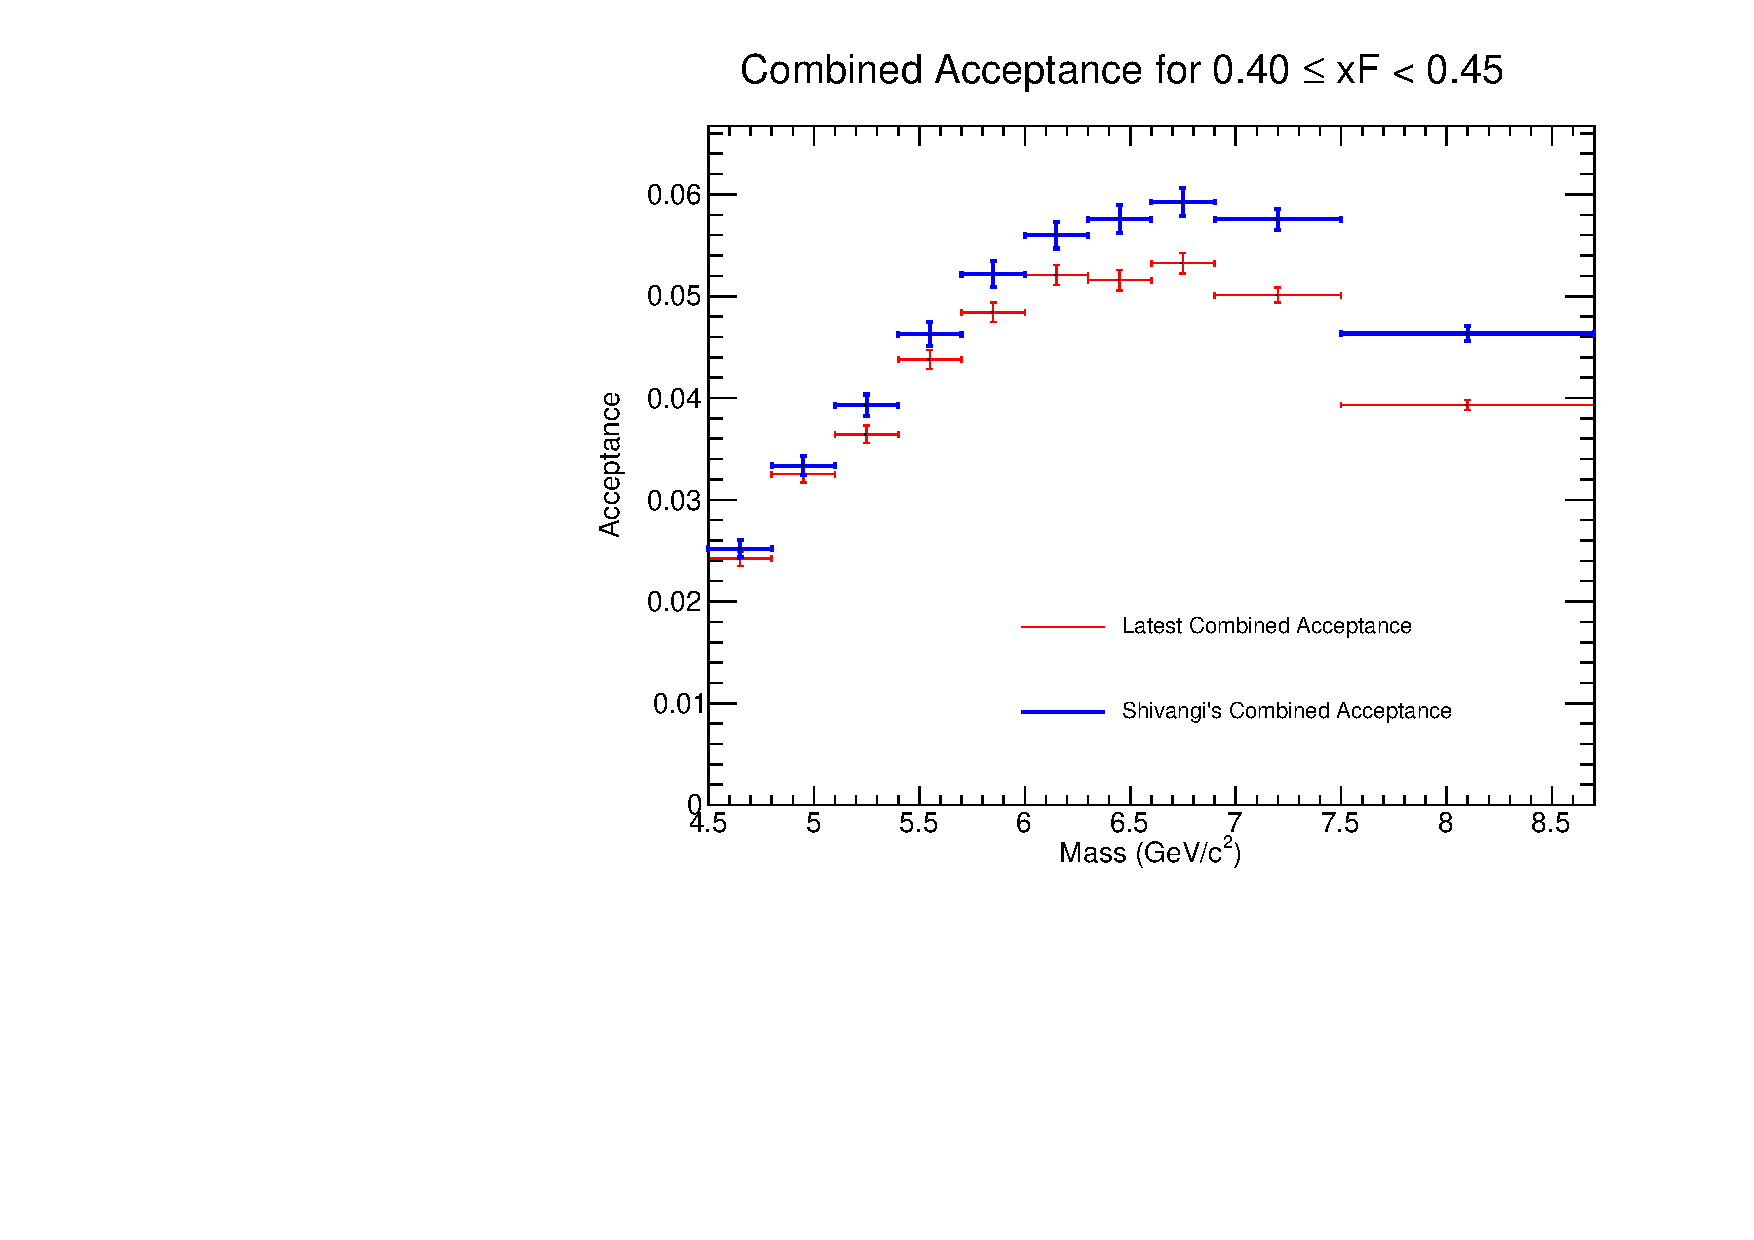
\includegraphics[width=\linewidth]{Combined_acceptance_xF_bin_8.pdf}
       \caption{Combined Acceptance}
    \end{subfigure}
    \hfill
    \begin{subfigure}[b]{0.48\textwidth}
       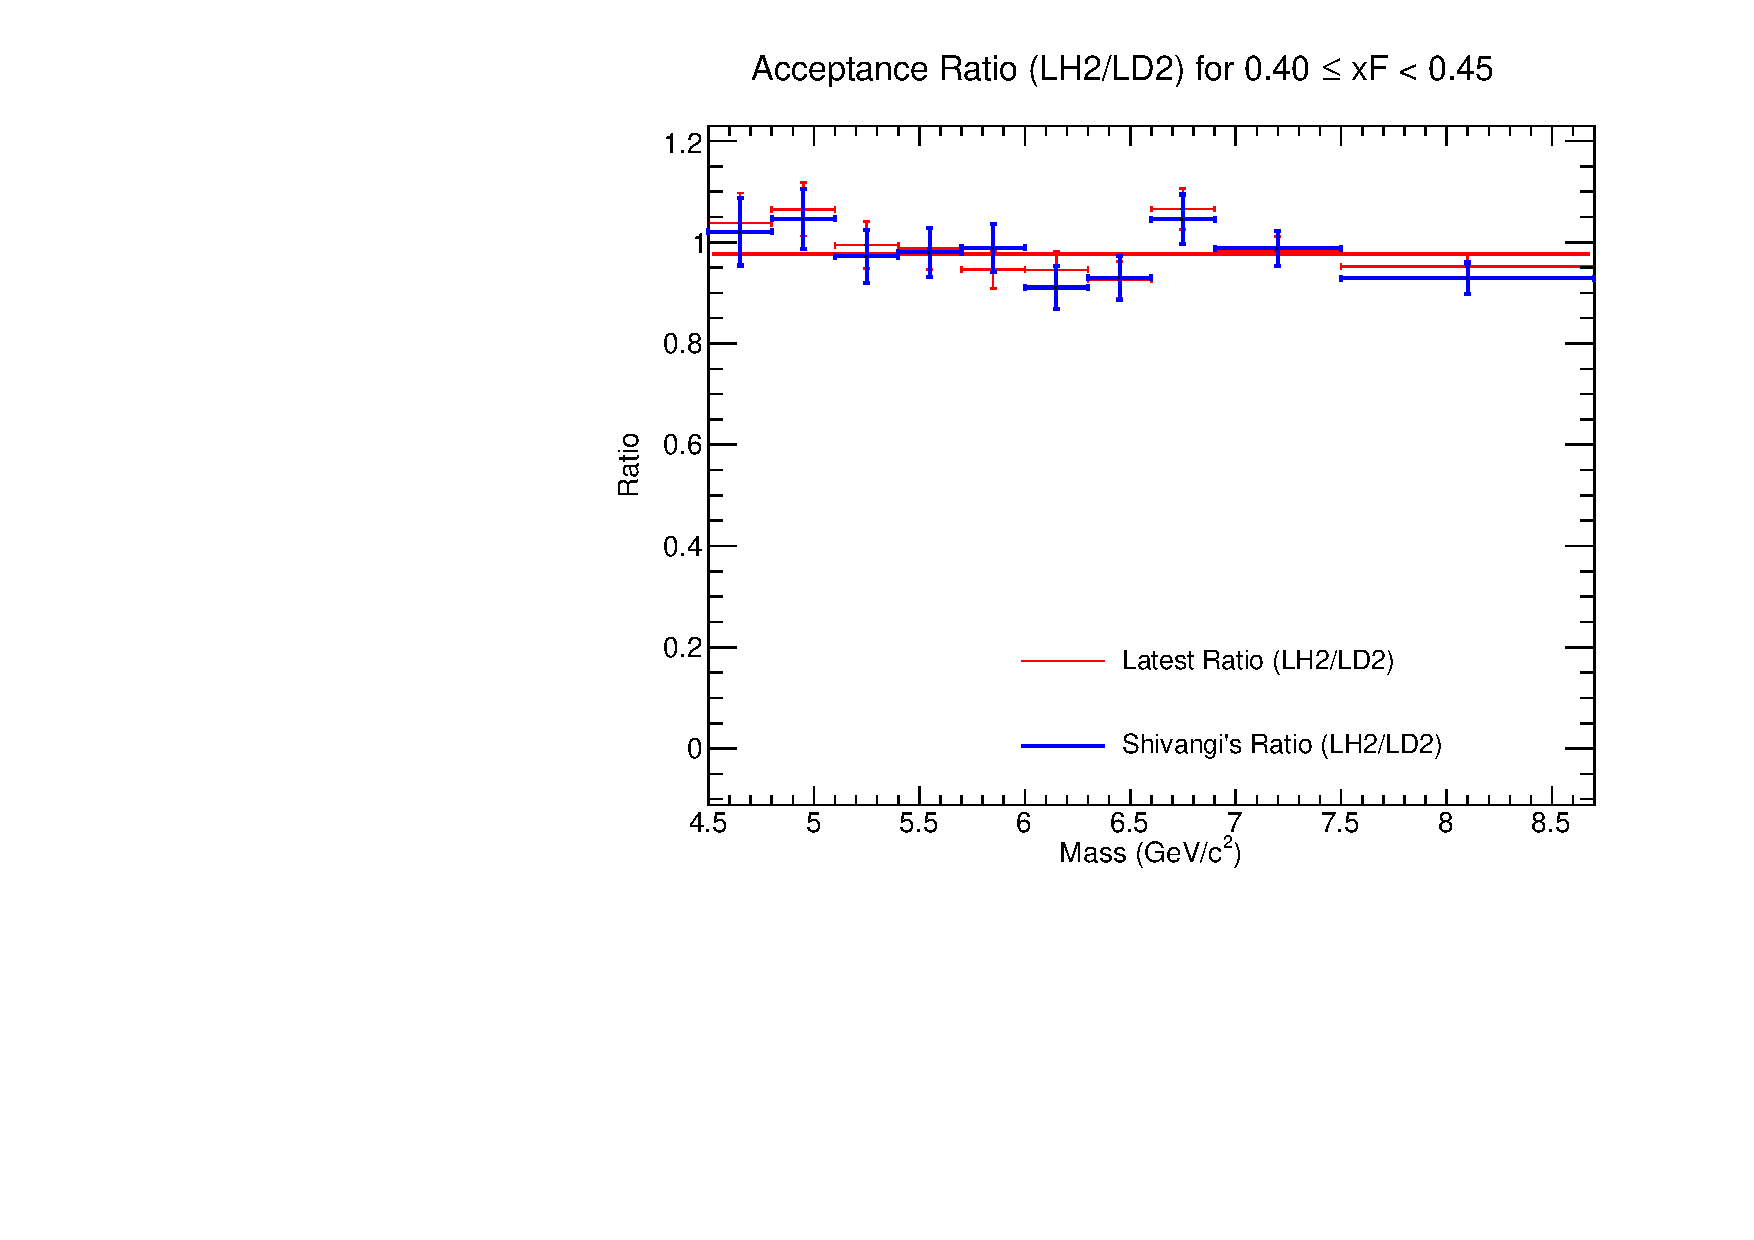
\includegraphics[width=\linewidth]{Acceptance_ratio_xF_bin_8.pdf}
       \caption{Acceptance Ratio (LH2/LD2)}
    \end{subfigure}
    \caption{Acceptance plots for $0.40 \le x_F < 0.45$.}
\end{figure}

\begin{figure}[H]
    \centering
    \begin{subfigure}[b]{0.48\textwidth}
       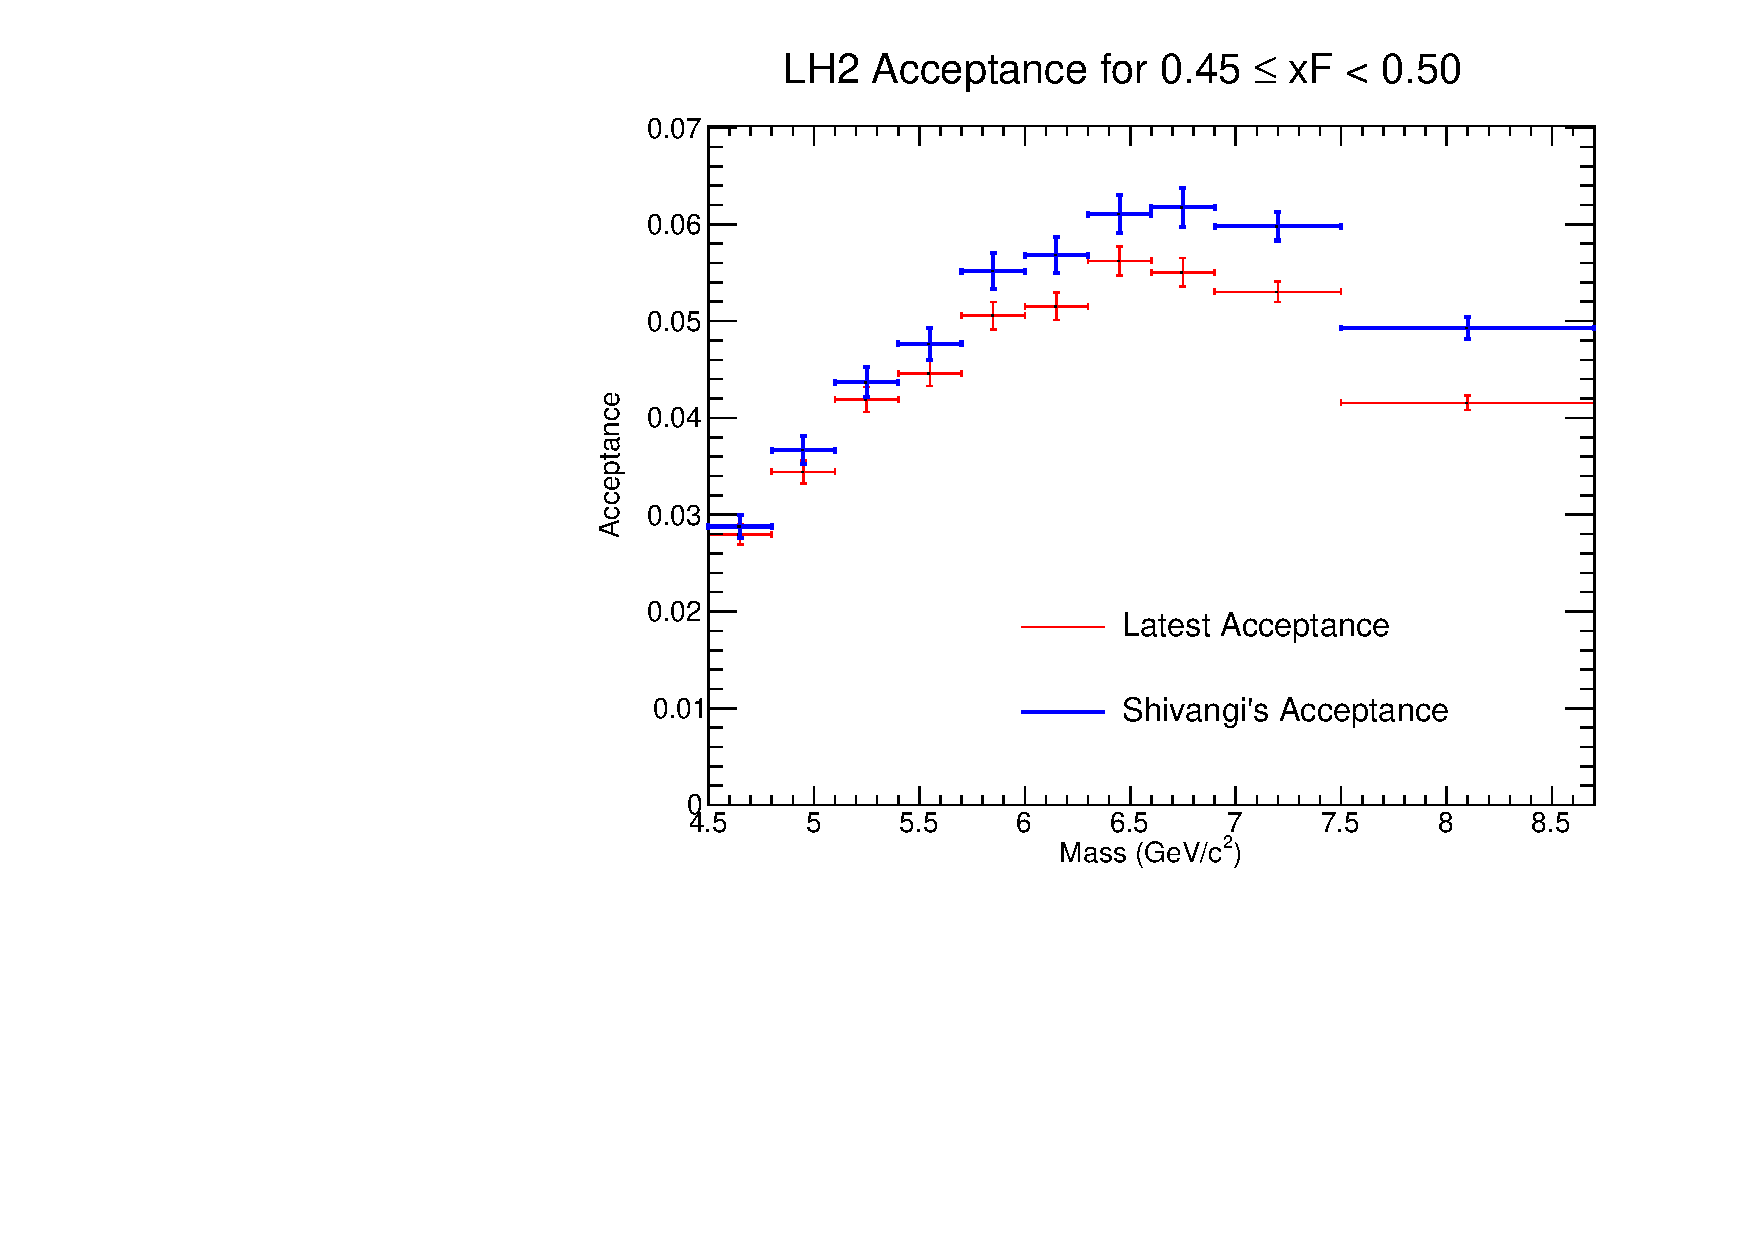
\includegraphics[width=\linewidth]{LH2_acceptance_xF_bin_9.pdf}
       \caption{Acceptance for LH2}
    \end{subfigure}
    \hfill
    \begin{subfigure}[b]{0.48\textwidth}
       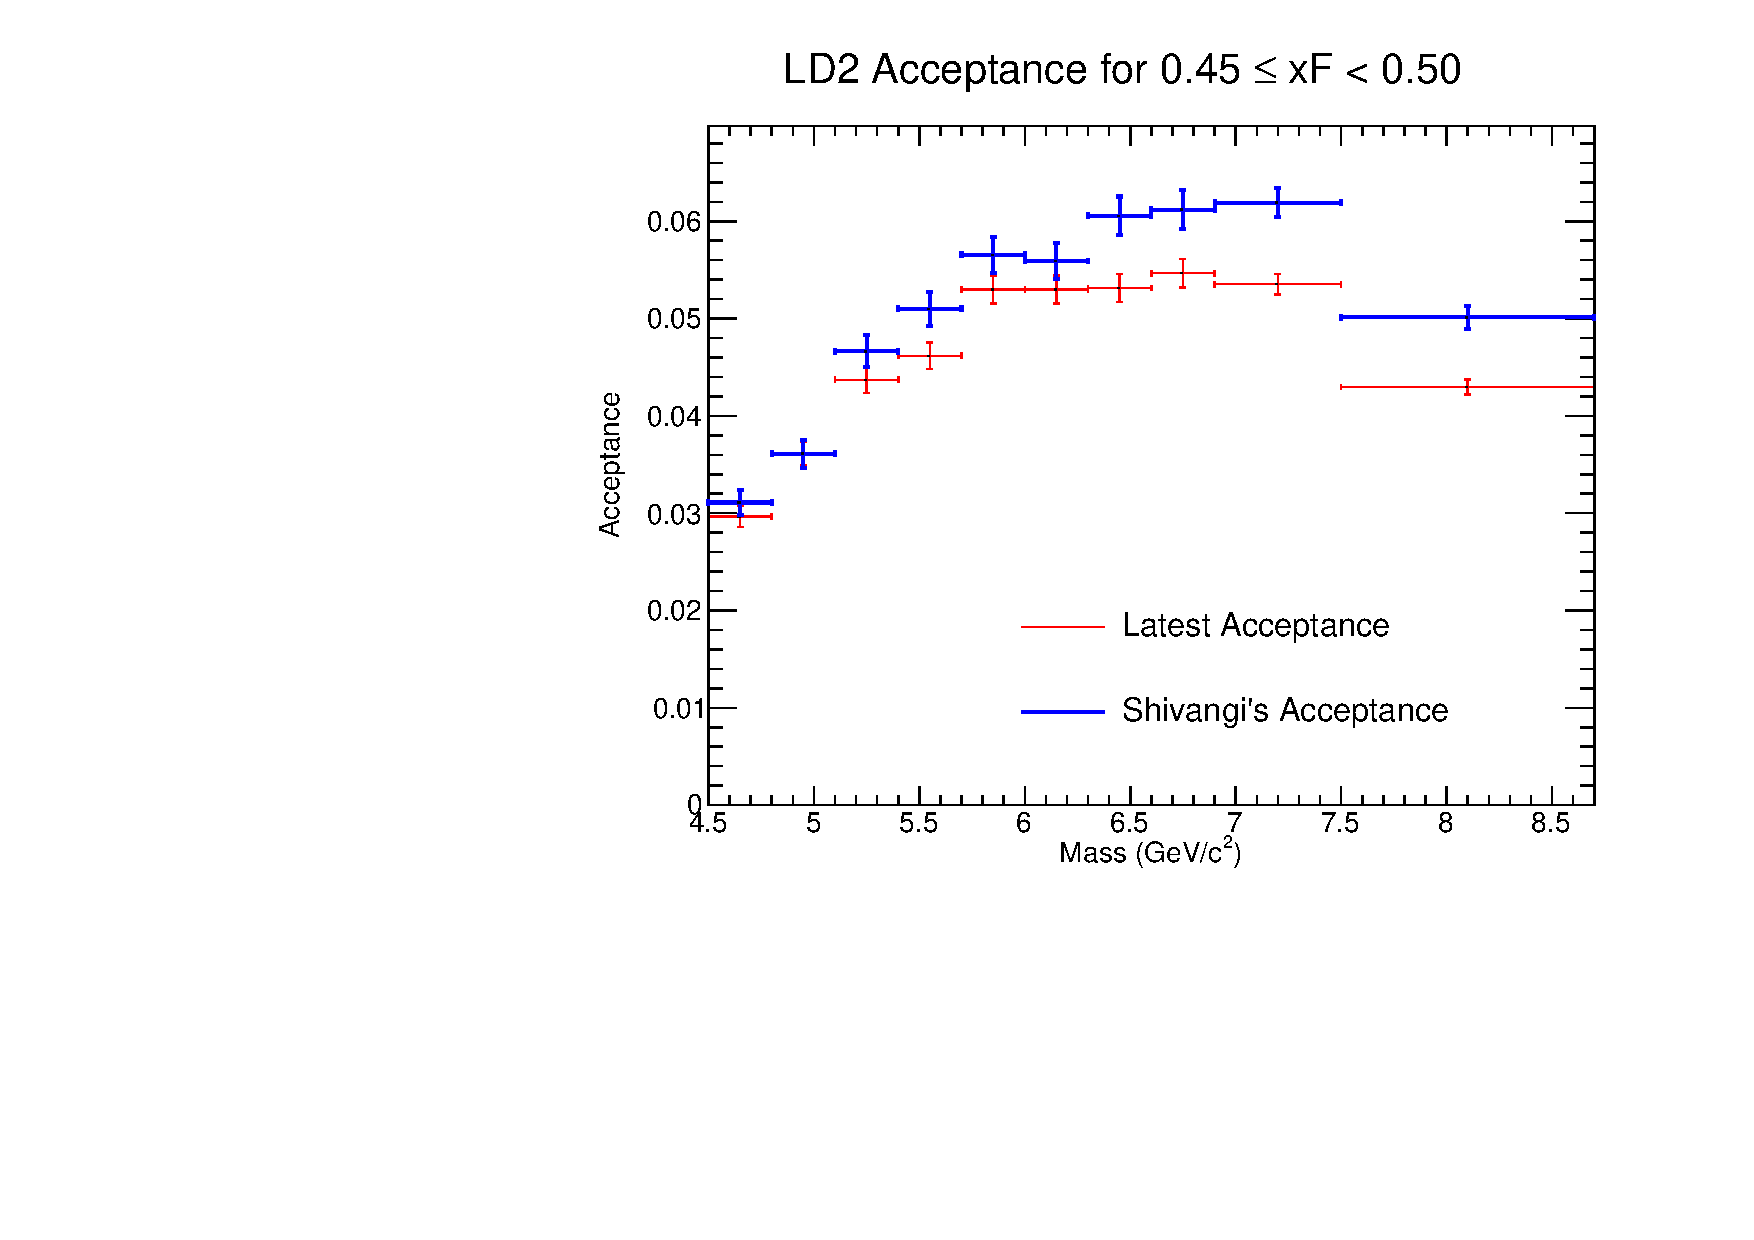
\includegraphics[width=\linewidth]{LD2_acceptance_xF_bin_9.pdf}
       \caption{Acceptance for LD2}
    \end{subfigure}

    \begin{subfigure}[b]{0.48\textwidth}
       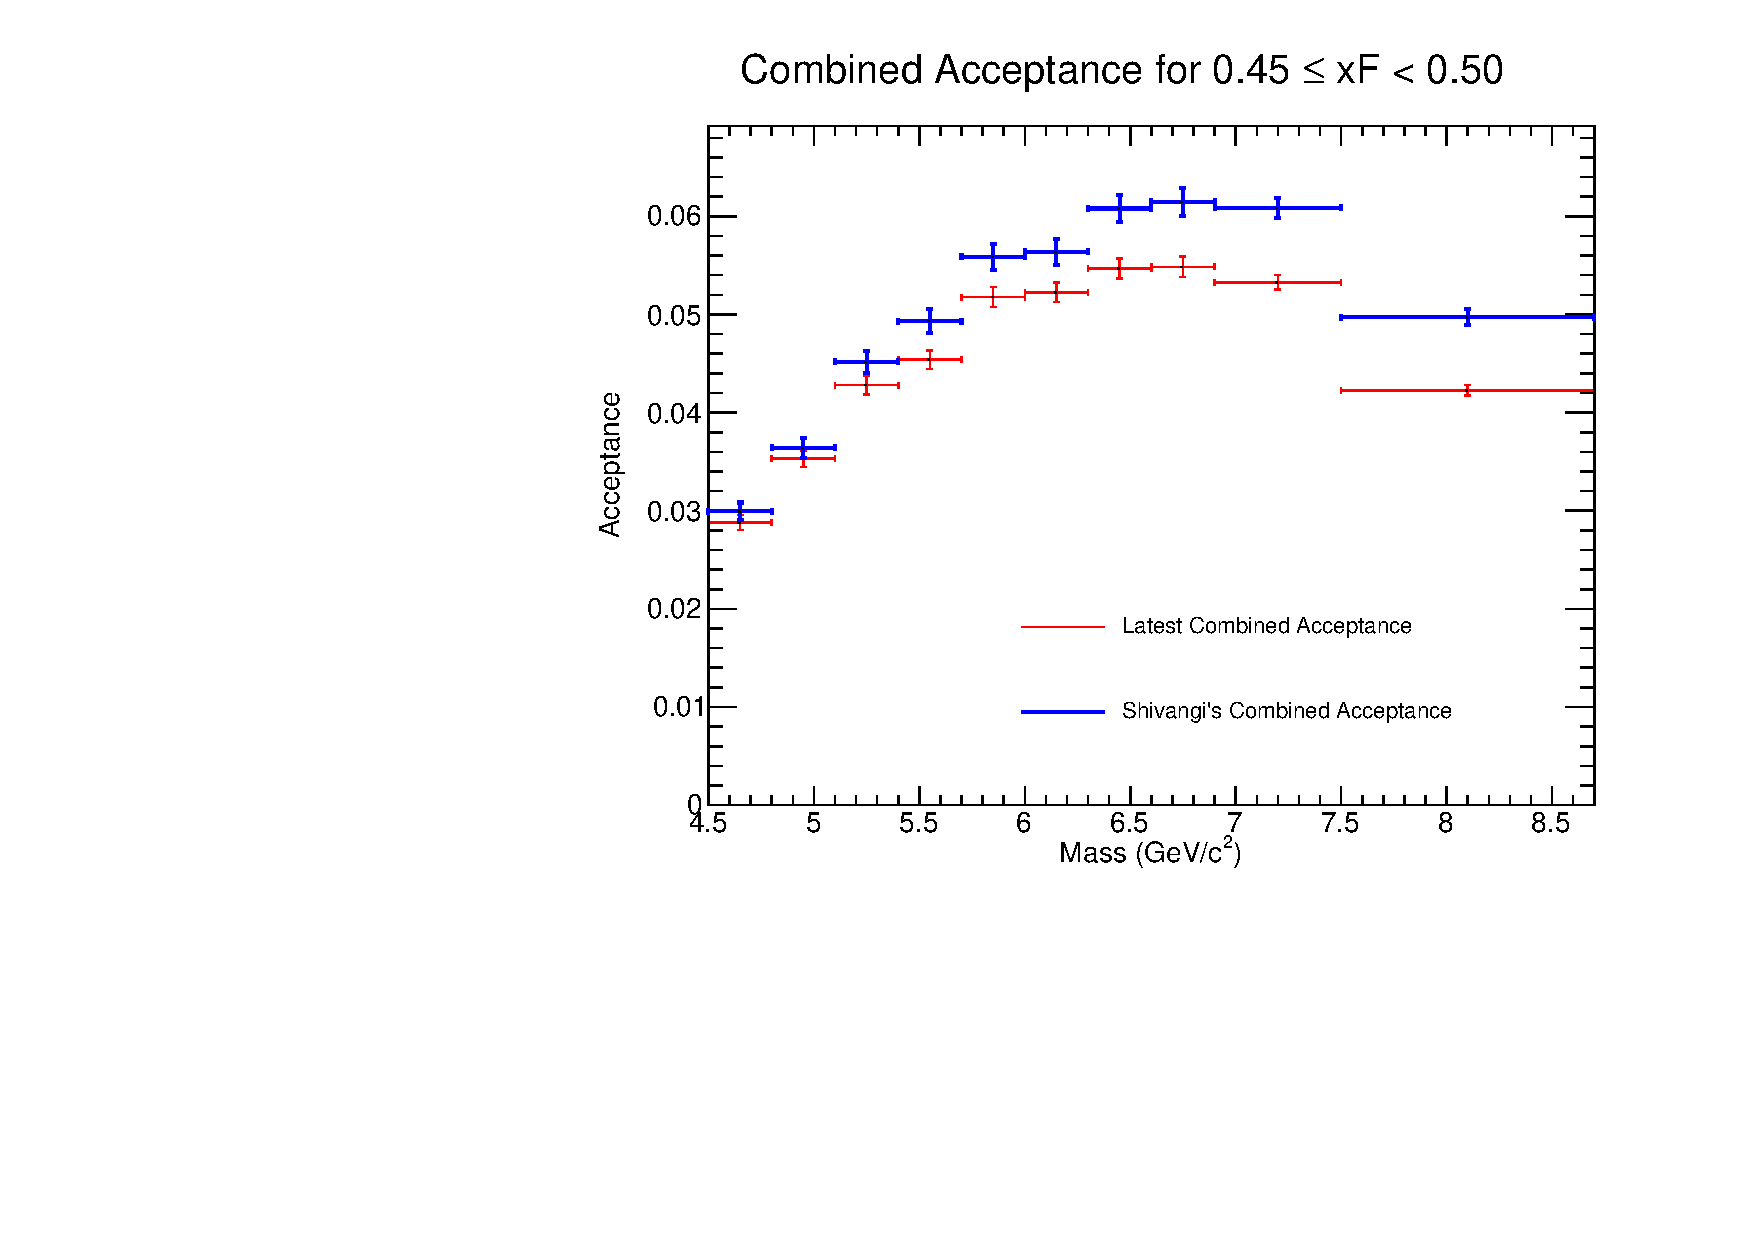
\includegraphics[width=\linewidth]{Combined_acceptance_xF_bin_9.pdf}
       \caption{Combined Acceptance}
    \end{subfigure}
    \hfill
    \begin{subfigure}[b]{0.48\textwidth}
       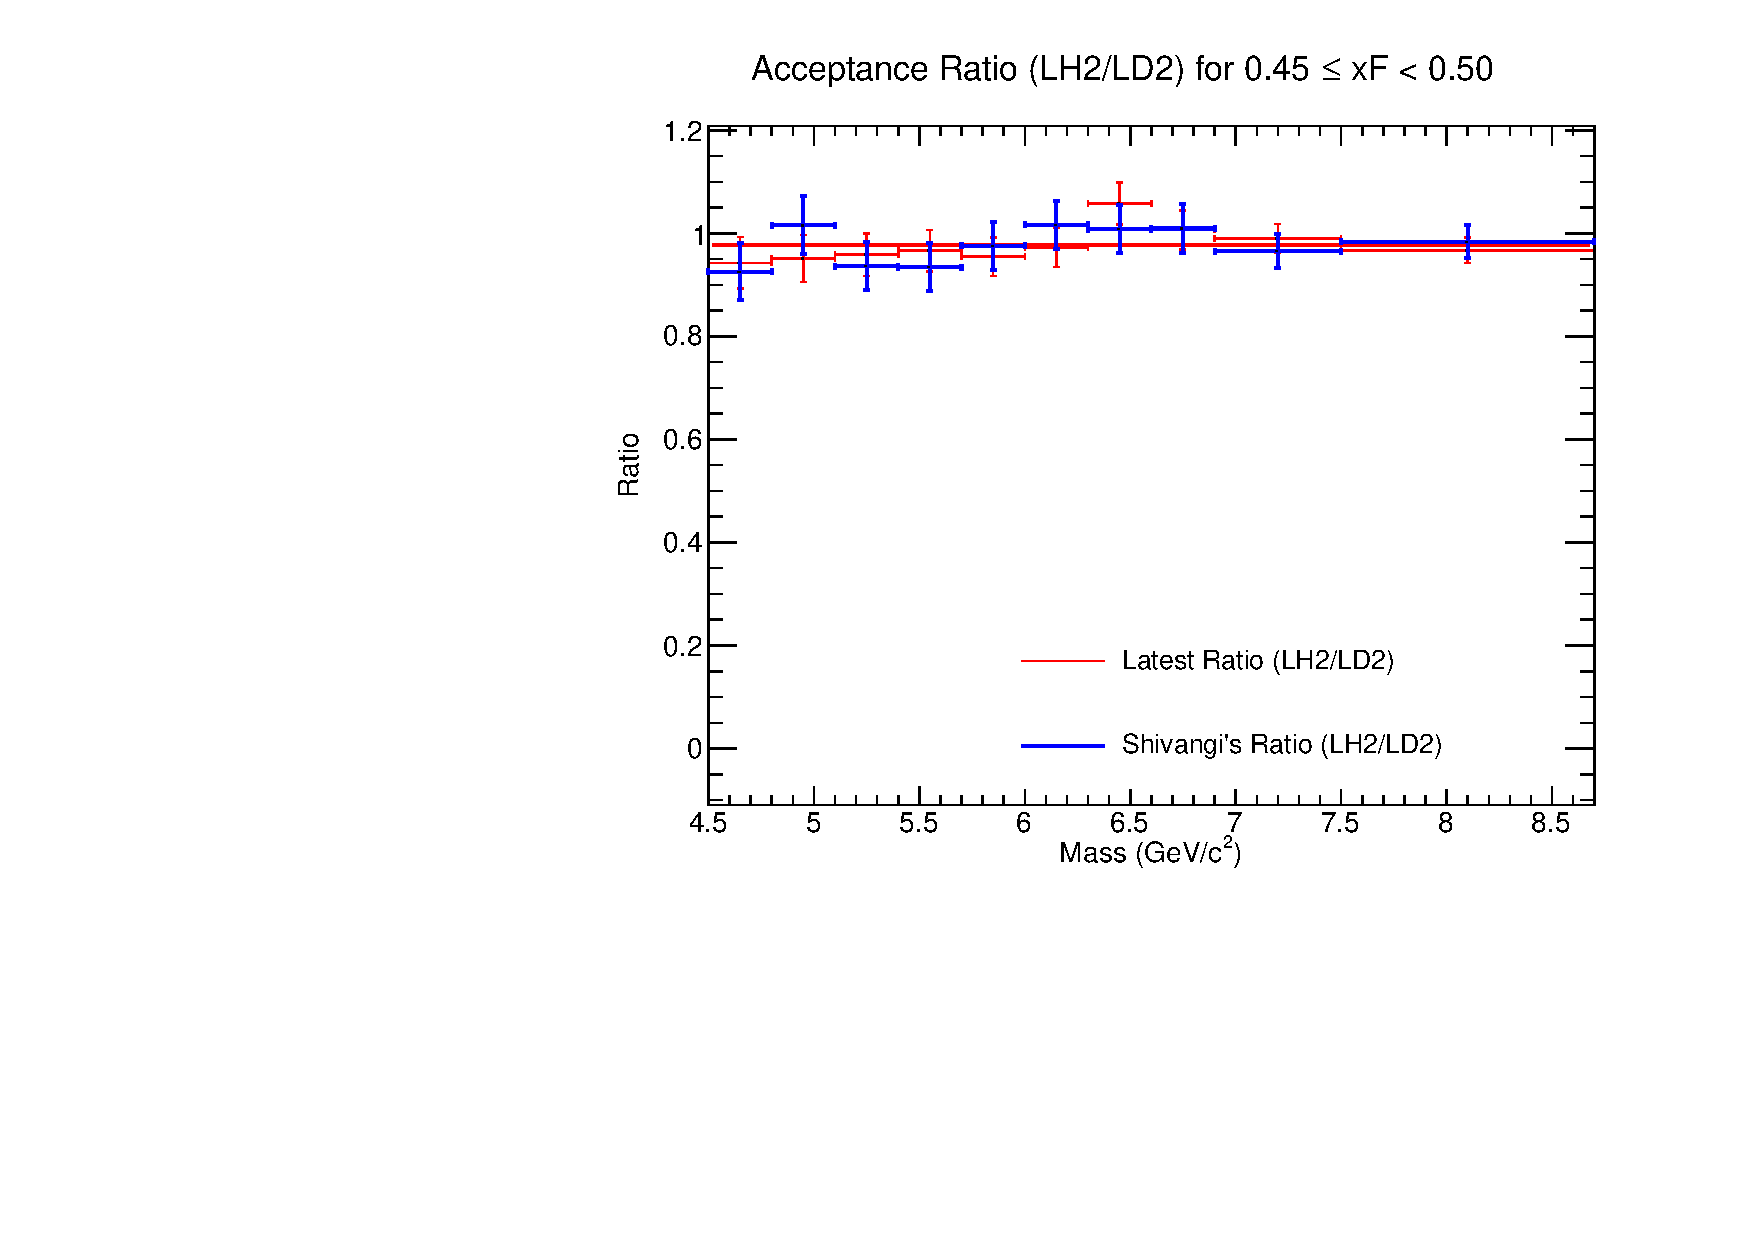
\includegraphics[width=\linewidth]{Acceptance_ratio_xF_bin_9.pdf}
       \caption{Acceptance Ratio (LH2/LD2)}
    \end{subfigure}
    \caption{Acceptance plots for $0.45 \le x_F < 0.50$.}
\end{figure}

\begin{figure}[H]
    \centering
    \begin{subfigure}[b]{0.48\textwidth}
       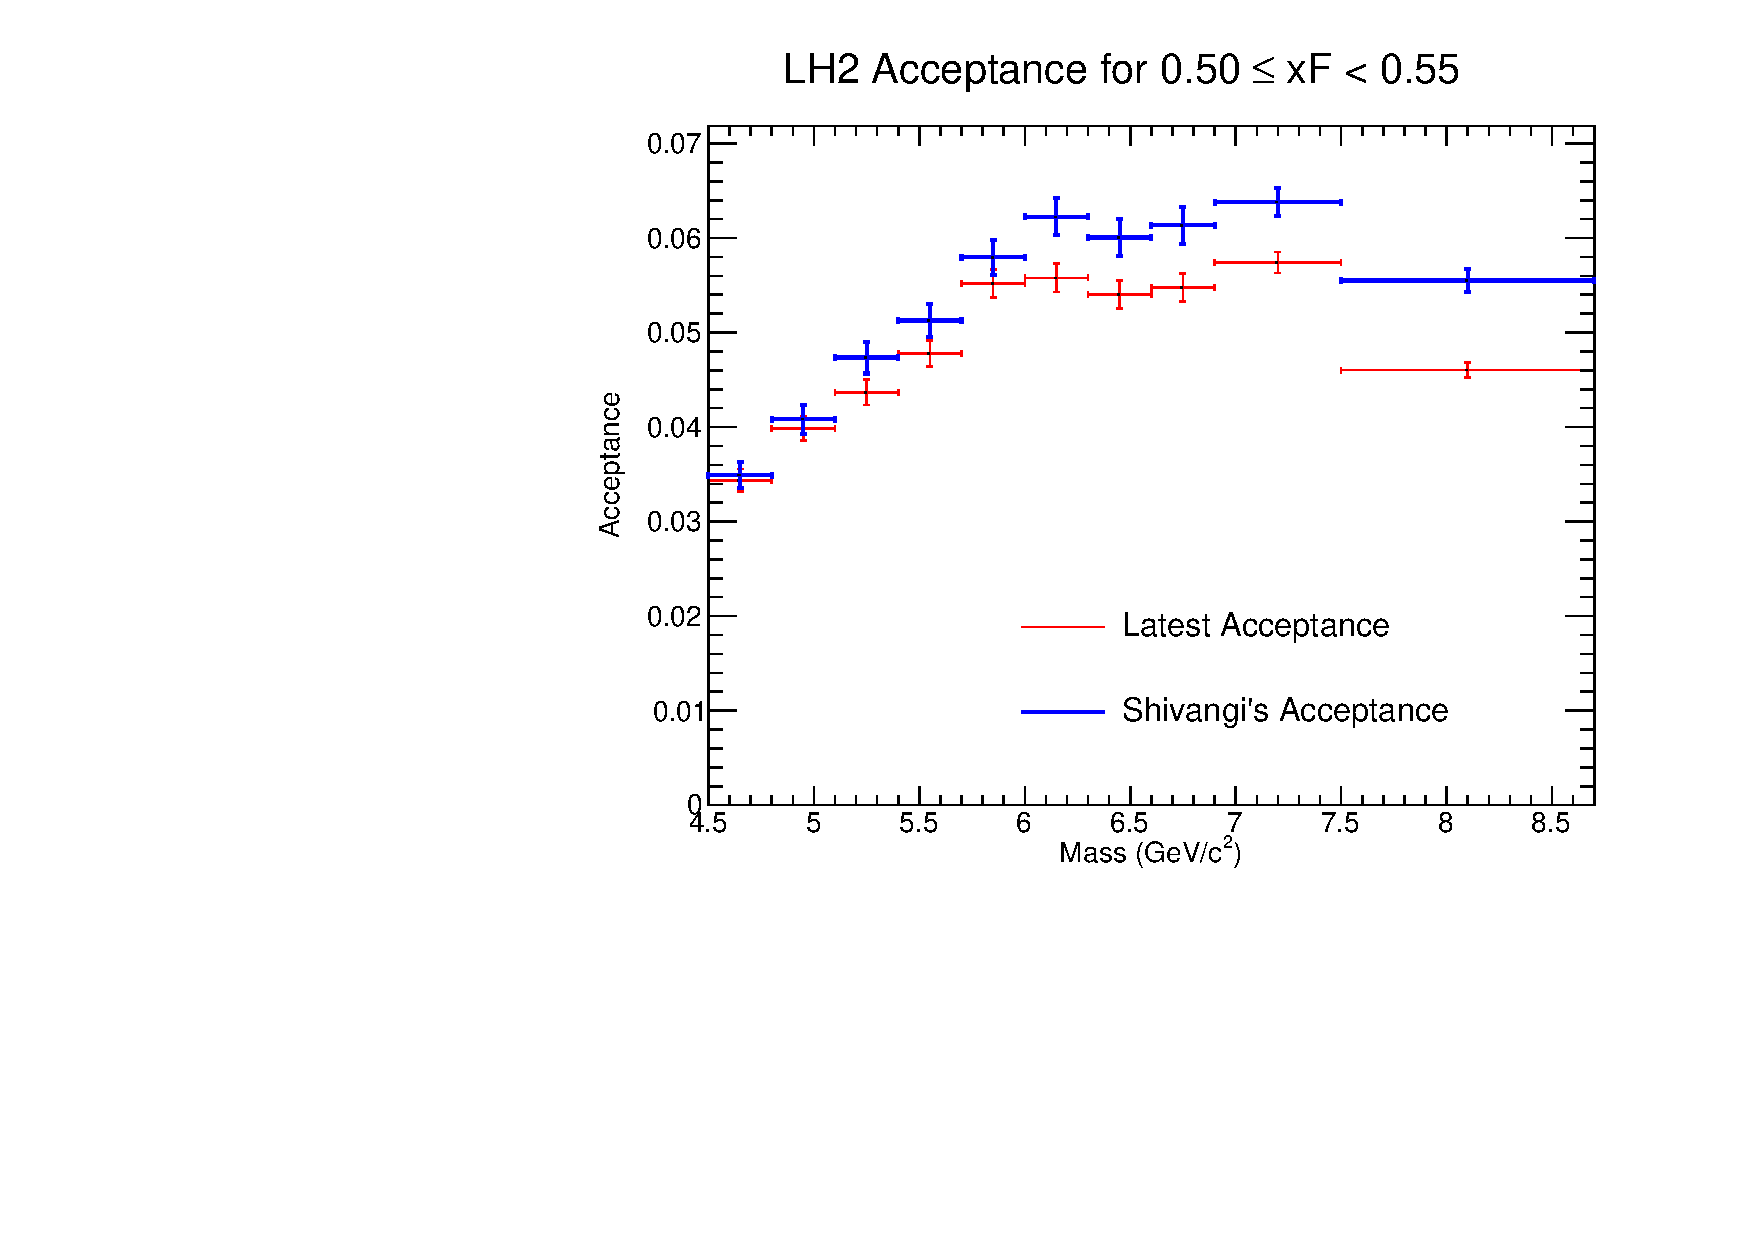
\includegraphics[width=\linewidth]{LH2_acceptance_xF_bin_10.pdf}
       \caption{Acceptance for LH2}
    \end{subfigure}
    \hfill
    \begin{subfigure}[b]{0.48\textwidth}
       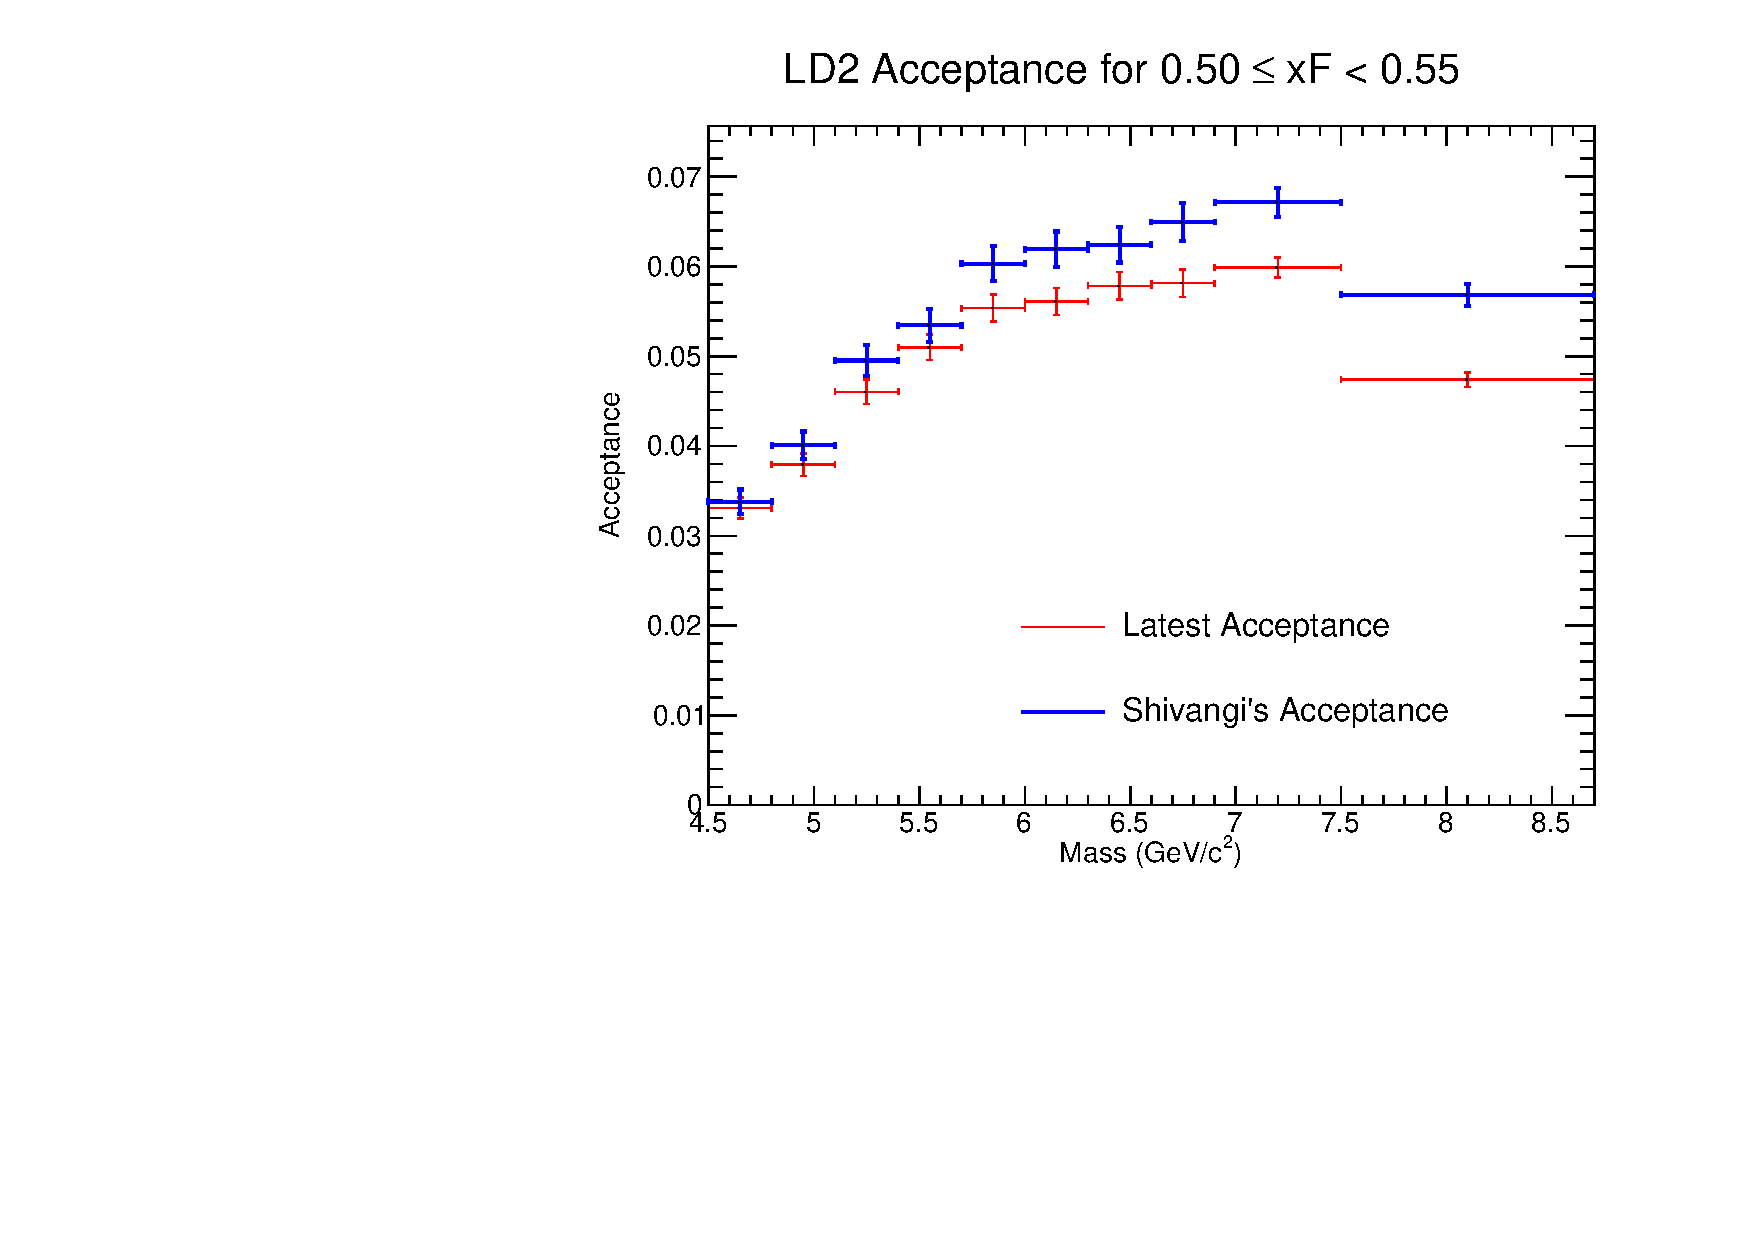
\includegraphics[width=\linewidth]{LD2_acceptance_xF_bin_10.pdf}
       \caption{Acceptance for LD2}
    \end{subfigure}

    \begin{subfigure}[b]{0.48\textwidth}
       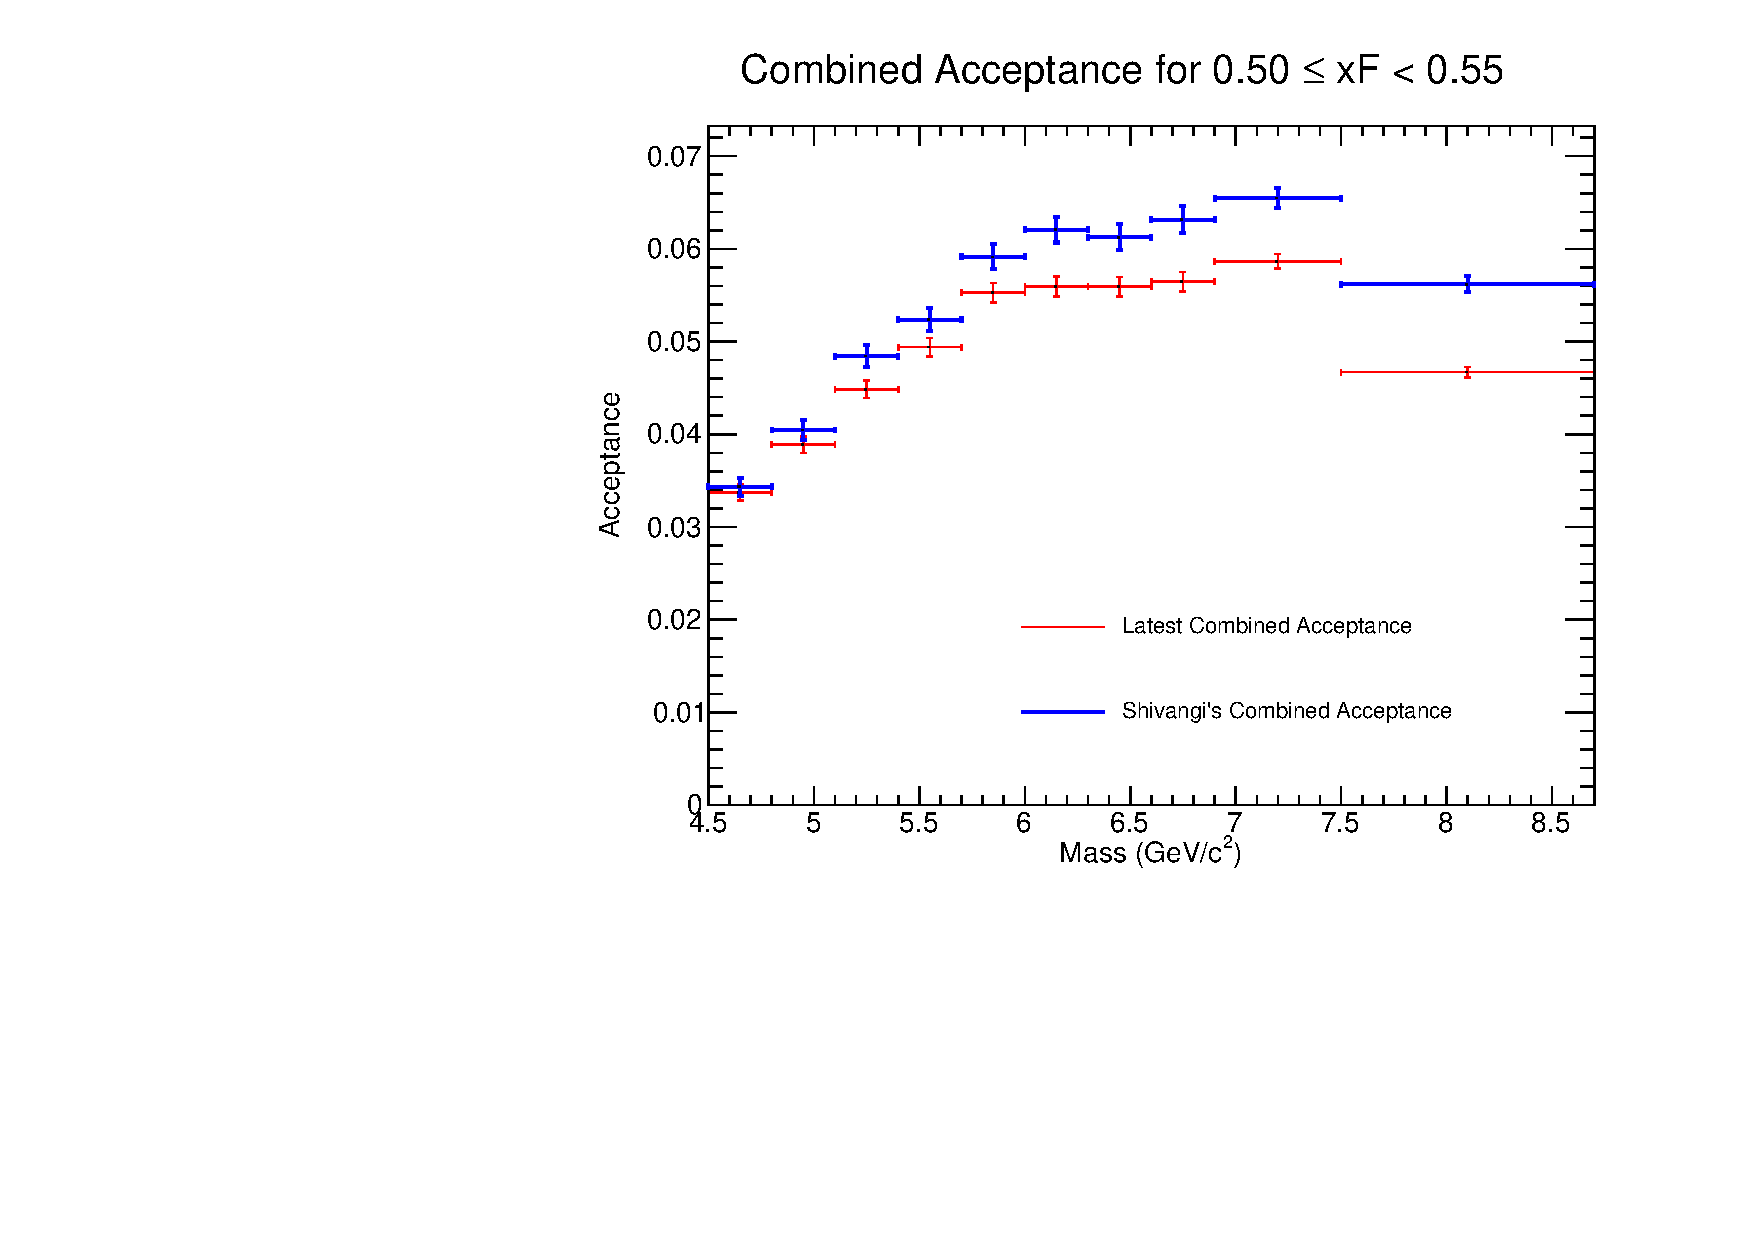
\includegraphics[width=\linewidth]{Combined_acceptance_xF_bin_10.pdf}
       \caption{Combined Acceptance}
    \end{subfigure}
    \hfill
    \begin{subfigure}[b]{0.48\textwidth}
       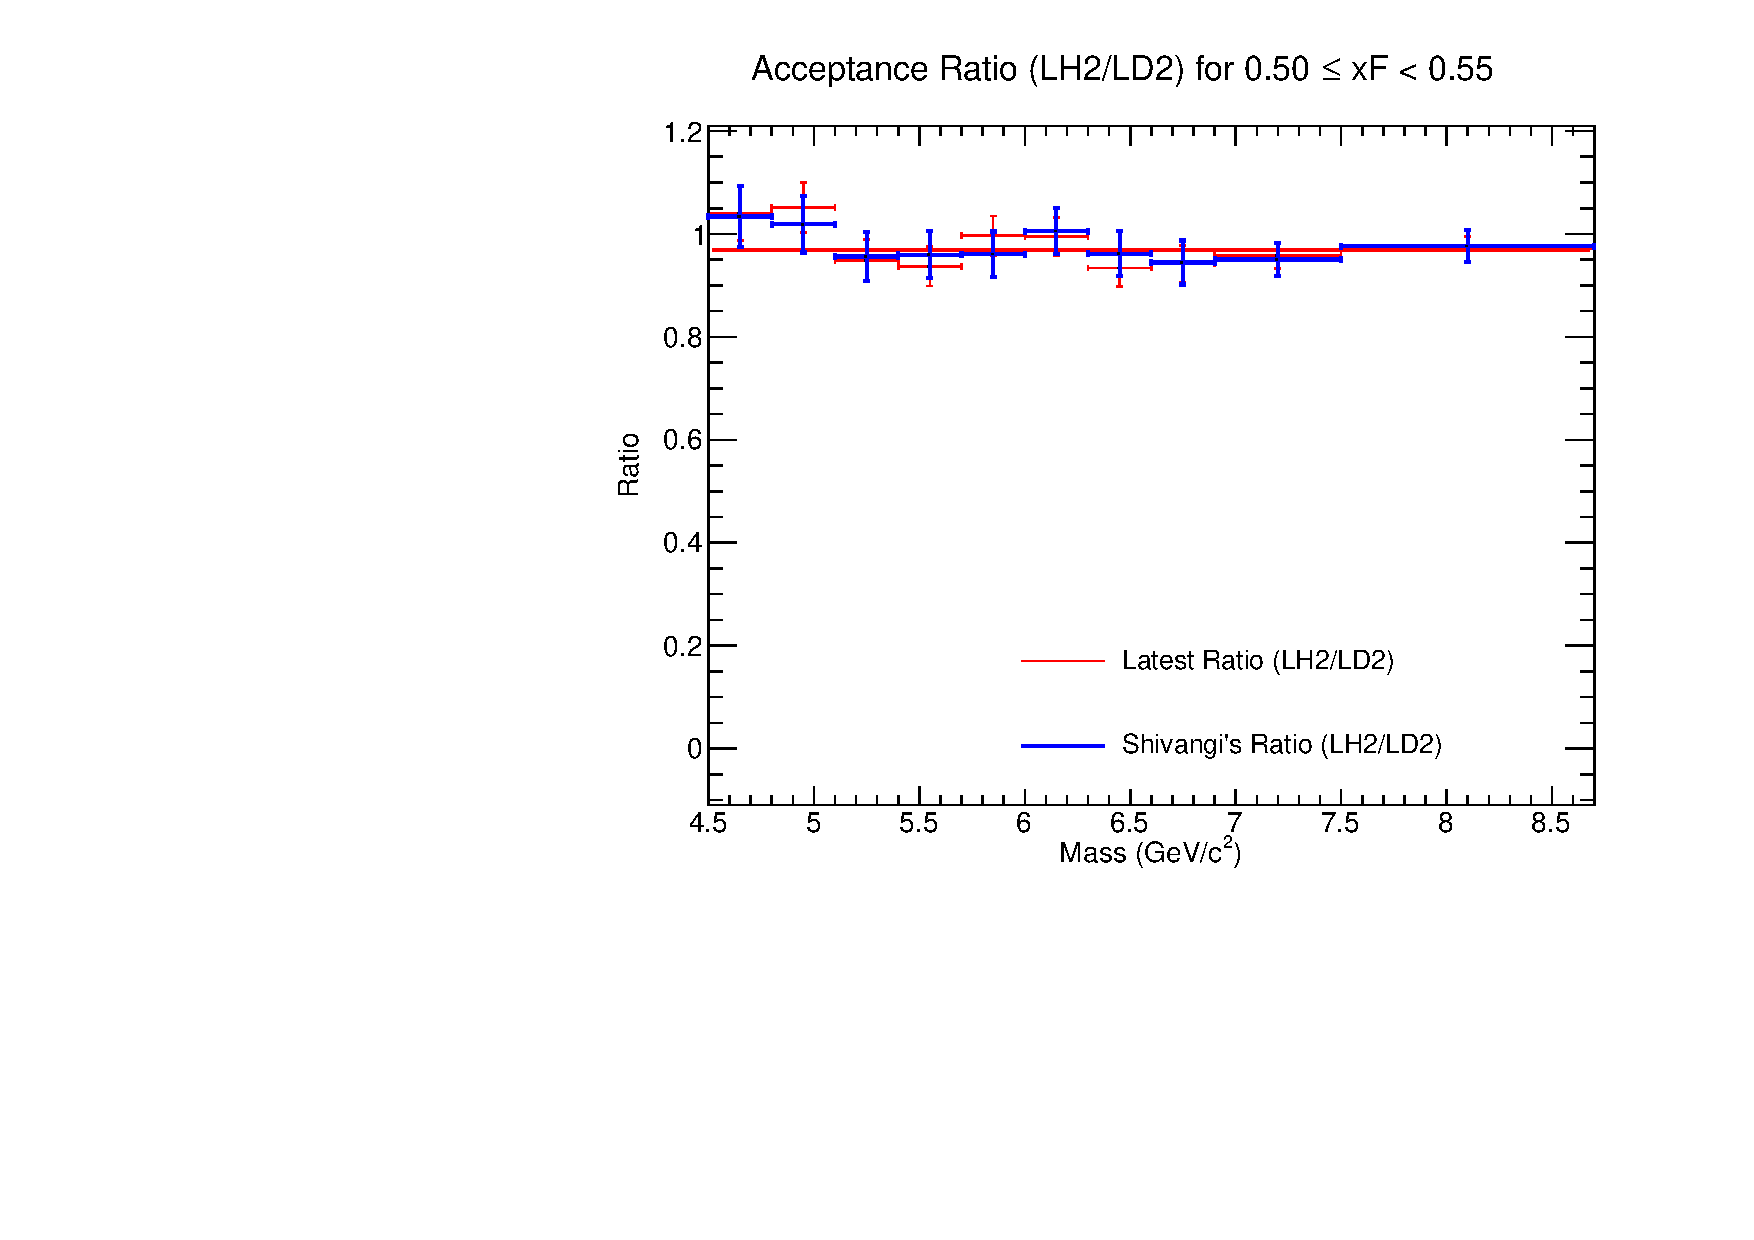
\includegraphics[width=\linewidth]{Acceptance_ratio_xF_bin_10.pdf}
       \caption{Acceptance Ratio (LH2/LD2)}
    \end{subfigure}
    \caption{Acceptance plots for $0.50 \le x_F < 0.55$.}
\end{figure}

\begin{figure}[H]
    \centering
    \begin{subfigure}[b]{0.48\textwidth}
       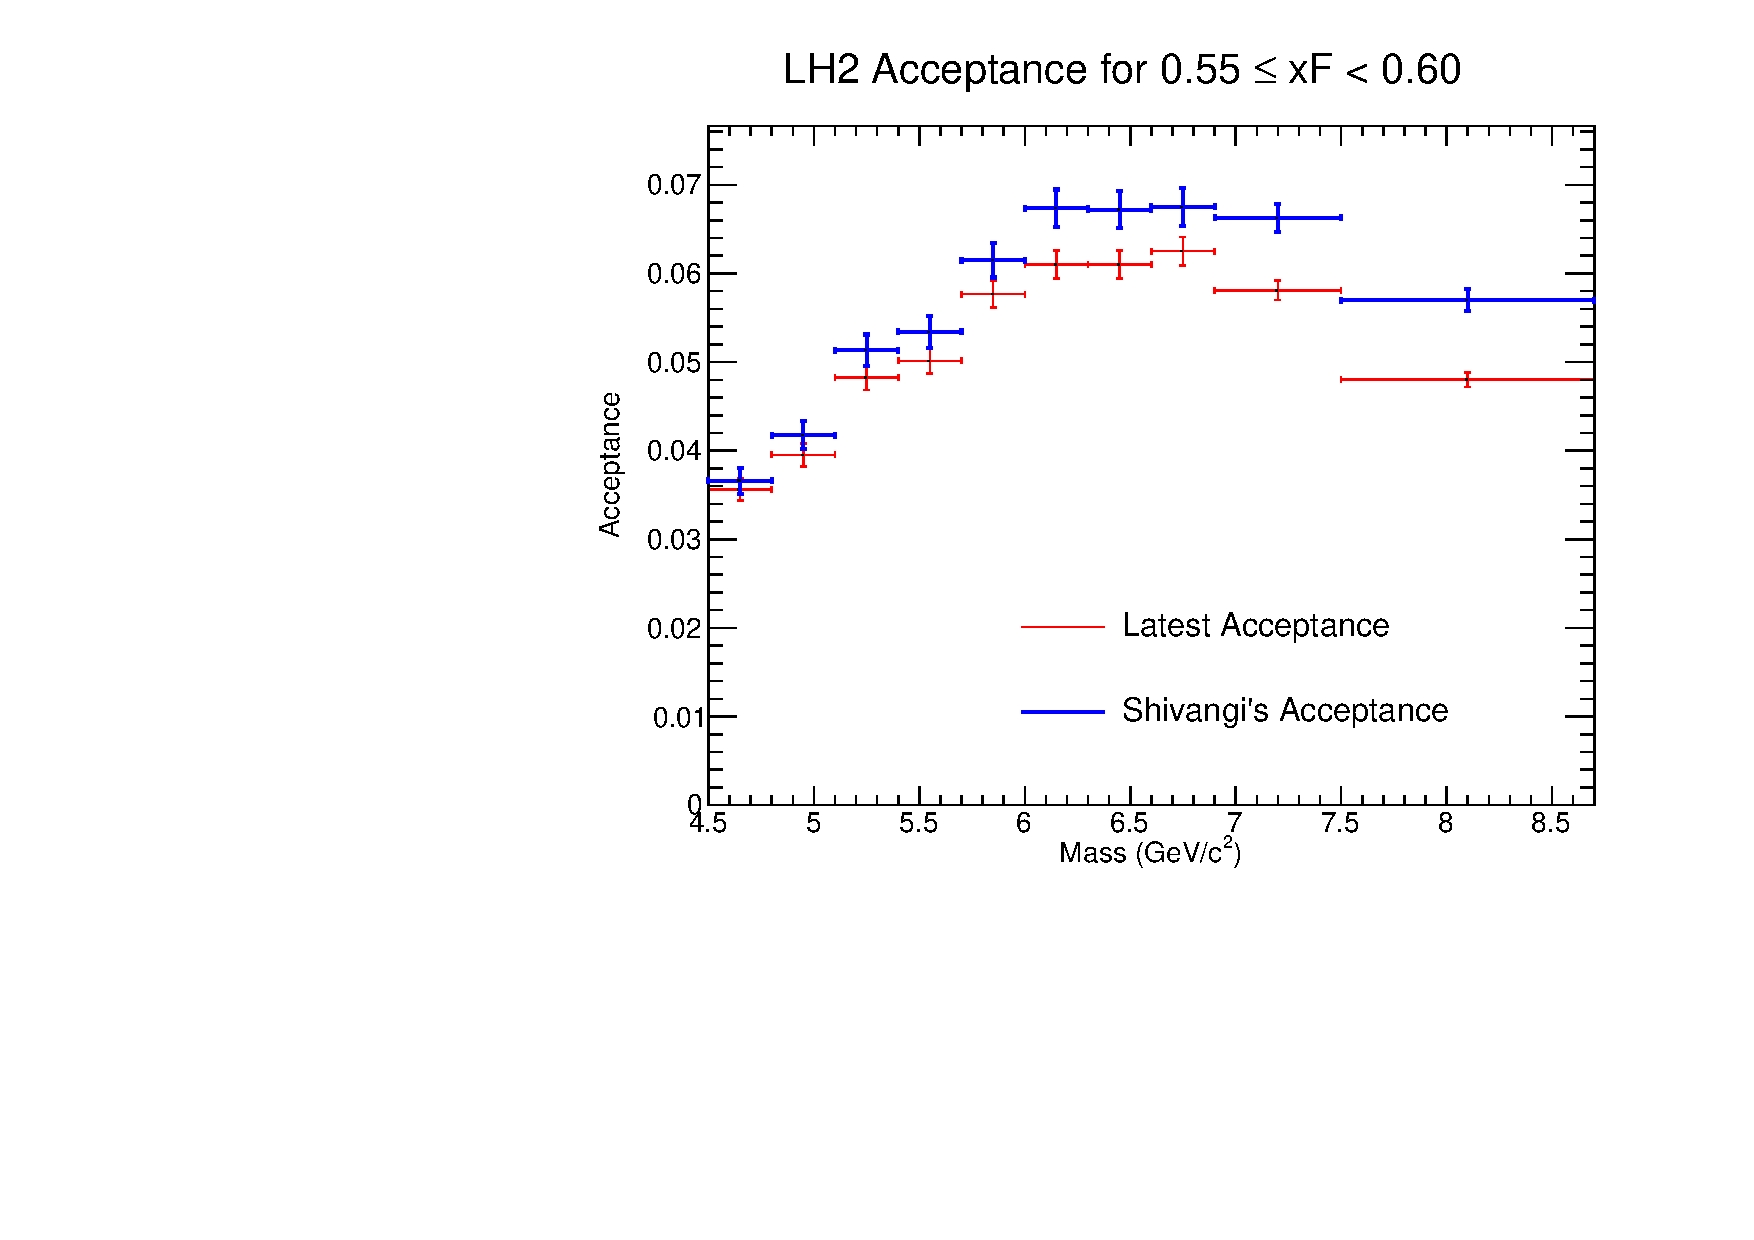
\includegraphics[width=\linewidth]{LH2_acceptance_xF_bin_11.pdf}
       \caption{Acceptance for LH2}
    \end{subfigure}
    \hfill
    \begin{subfigure}[b]{0.48\textwidth}
       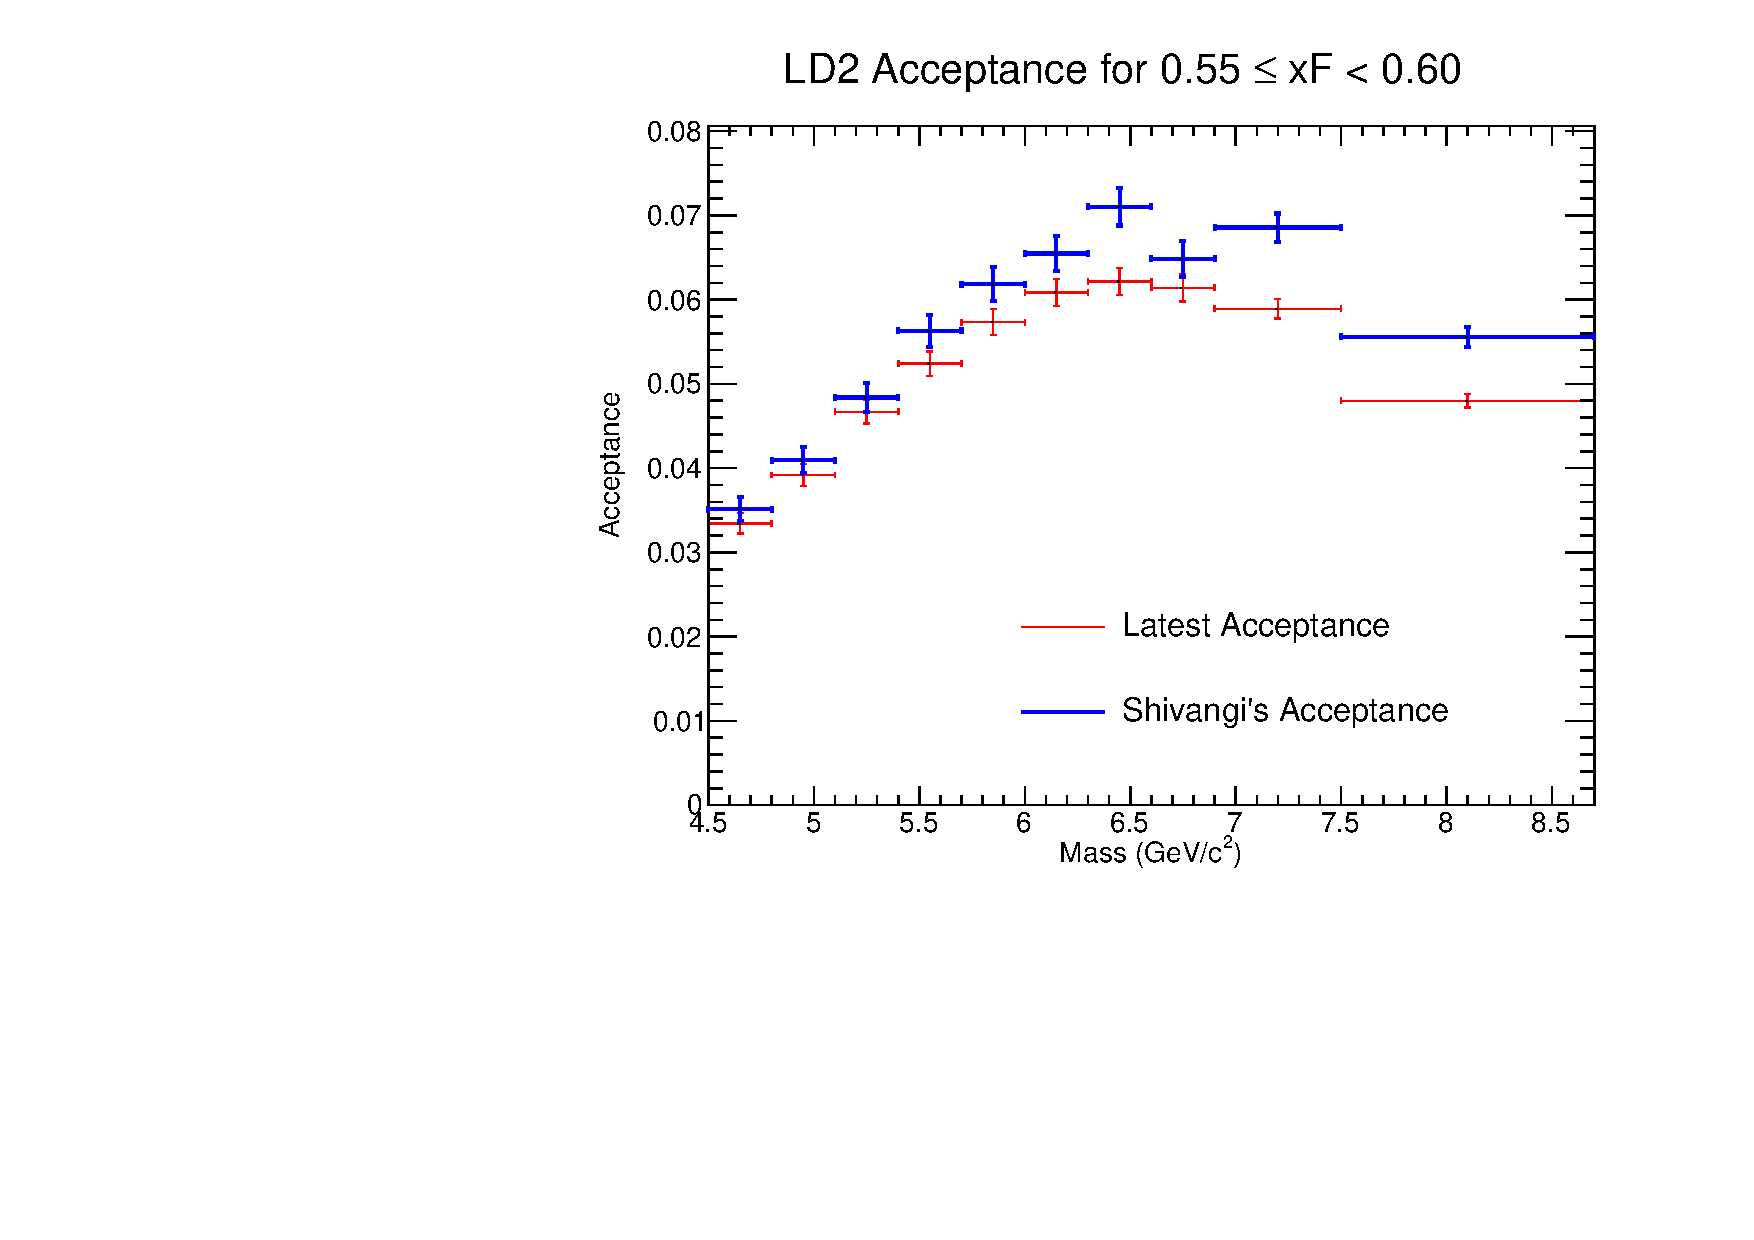
\includegraphics[width=\linewidth]{LD2_acceptance_xF_bin_11.pdf}
       \caption{Acceptance for LD2}
    \end{subfigure}

    \begin{subfigure}[b]{0.48\textwidth}
       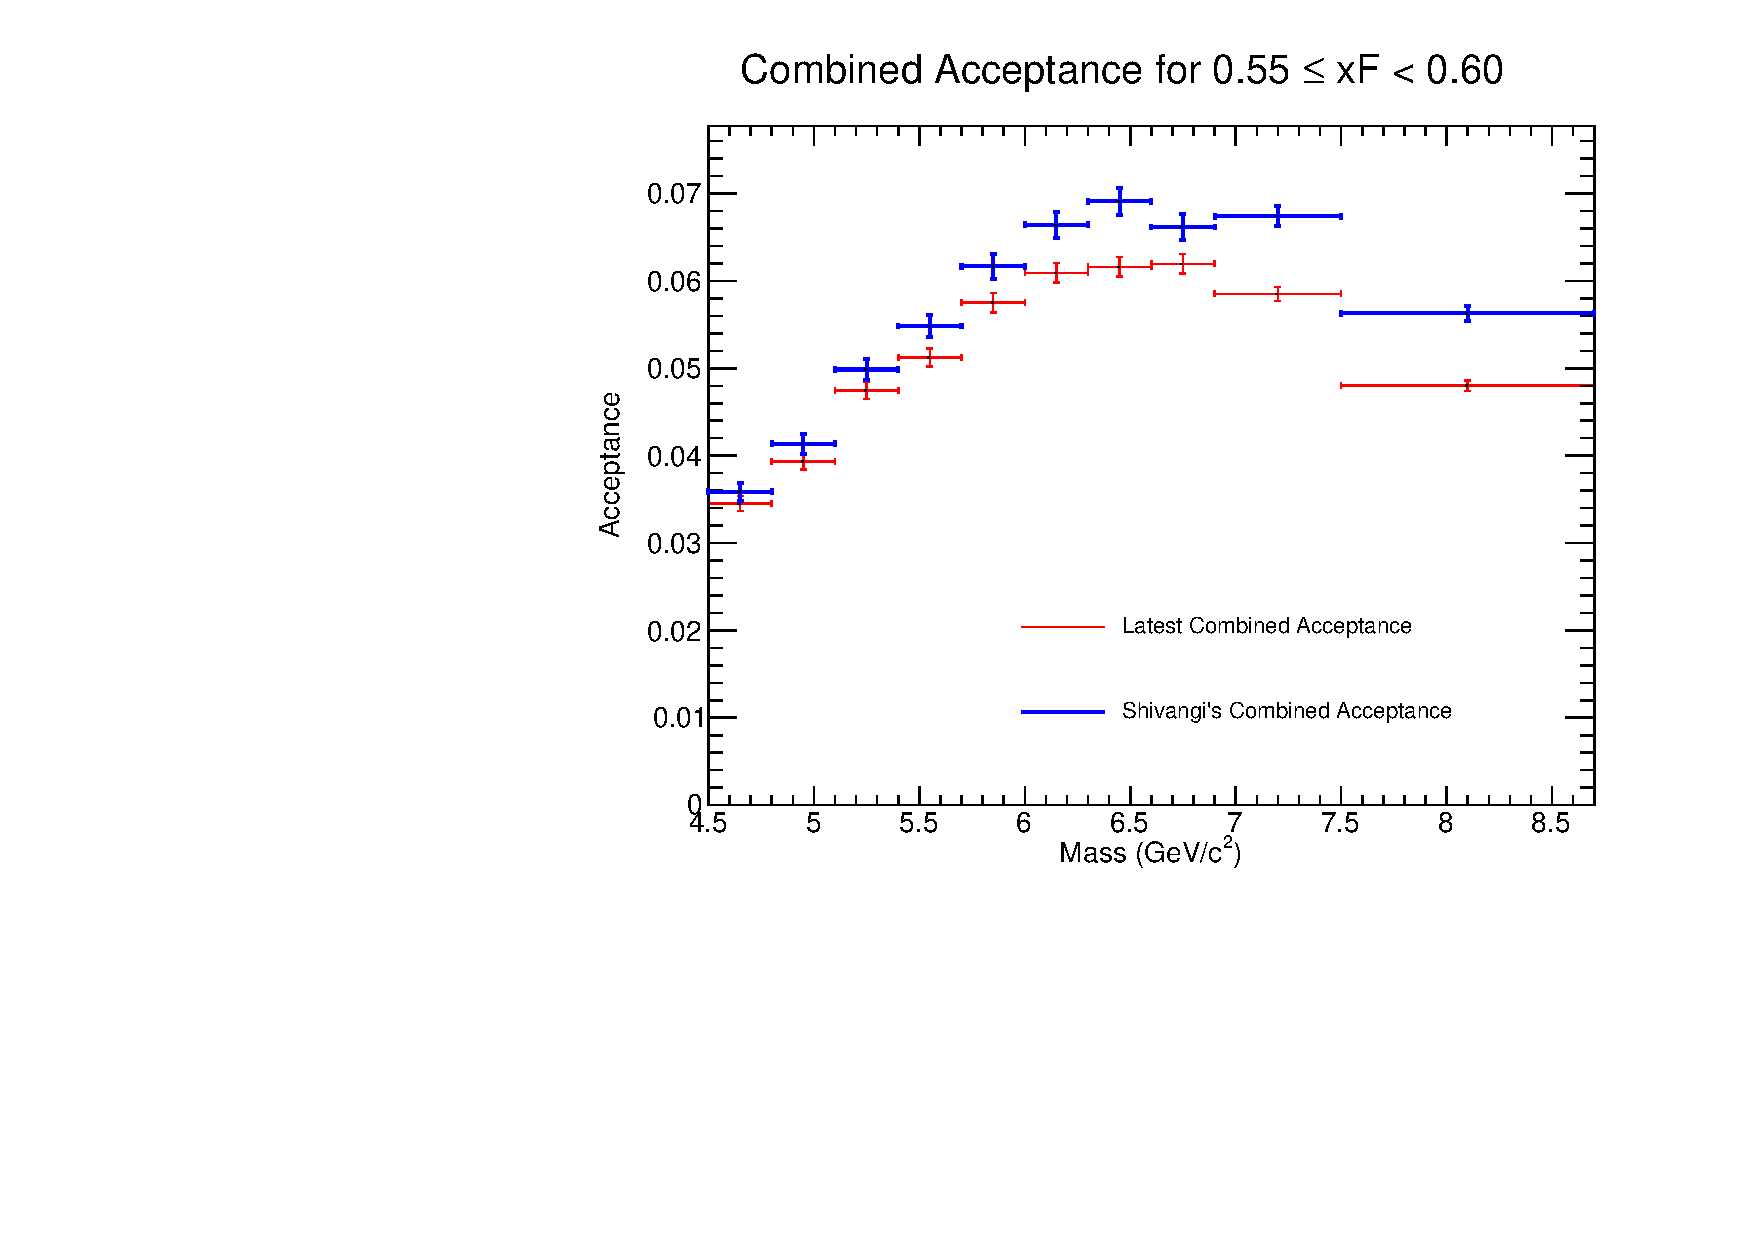
\includegraphics[width=\linewidth]{Combined_acceptance_xF_bin_11.pdf}
       \caption{Combined Acceptance}
    \end{subfigure}
    \hfill
    \begin{subfigure}[b]{0.48\textwidth}
       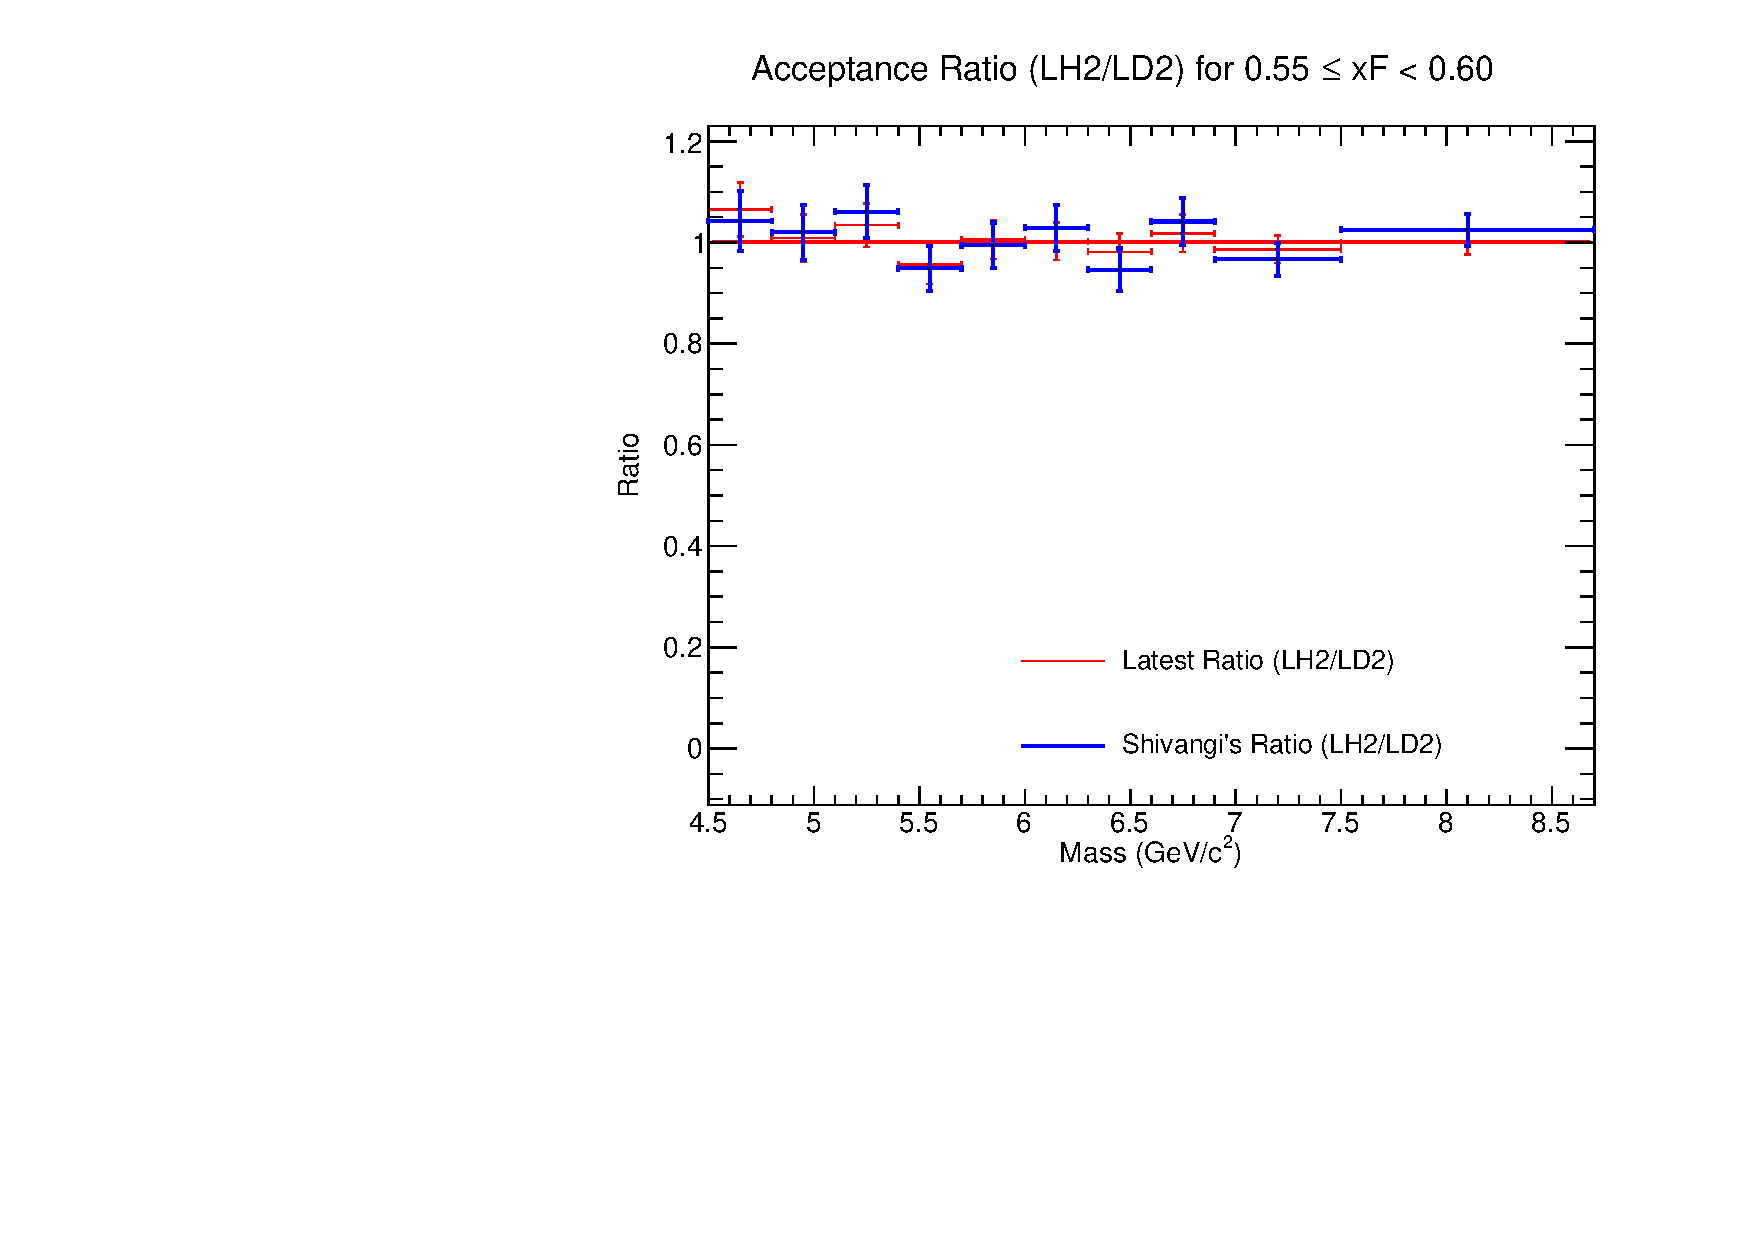
\includegraphics[width=\linewidth]{Acceptance_ratio_xF_bin_11.pdf}
       \caption{Acceptance Ratio (LH2/LD2)}
    \end{subfigure}
    \caption{Acceptance plots for $0.55 \le x_F < 0.60$.}
\end{figure}

\begin{figure}[H]
    \centering
    \begin{subfigure}[b]{0.48\textwidth}
       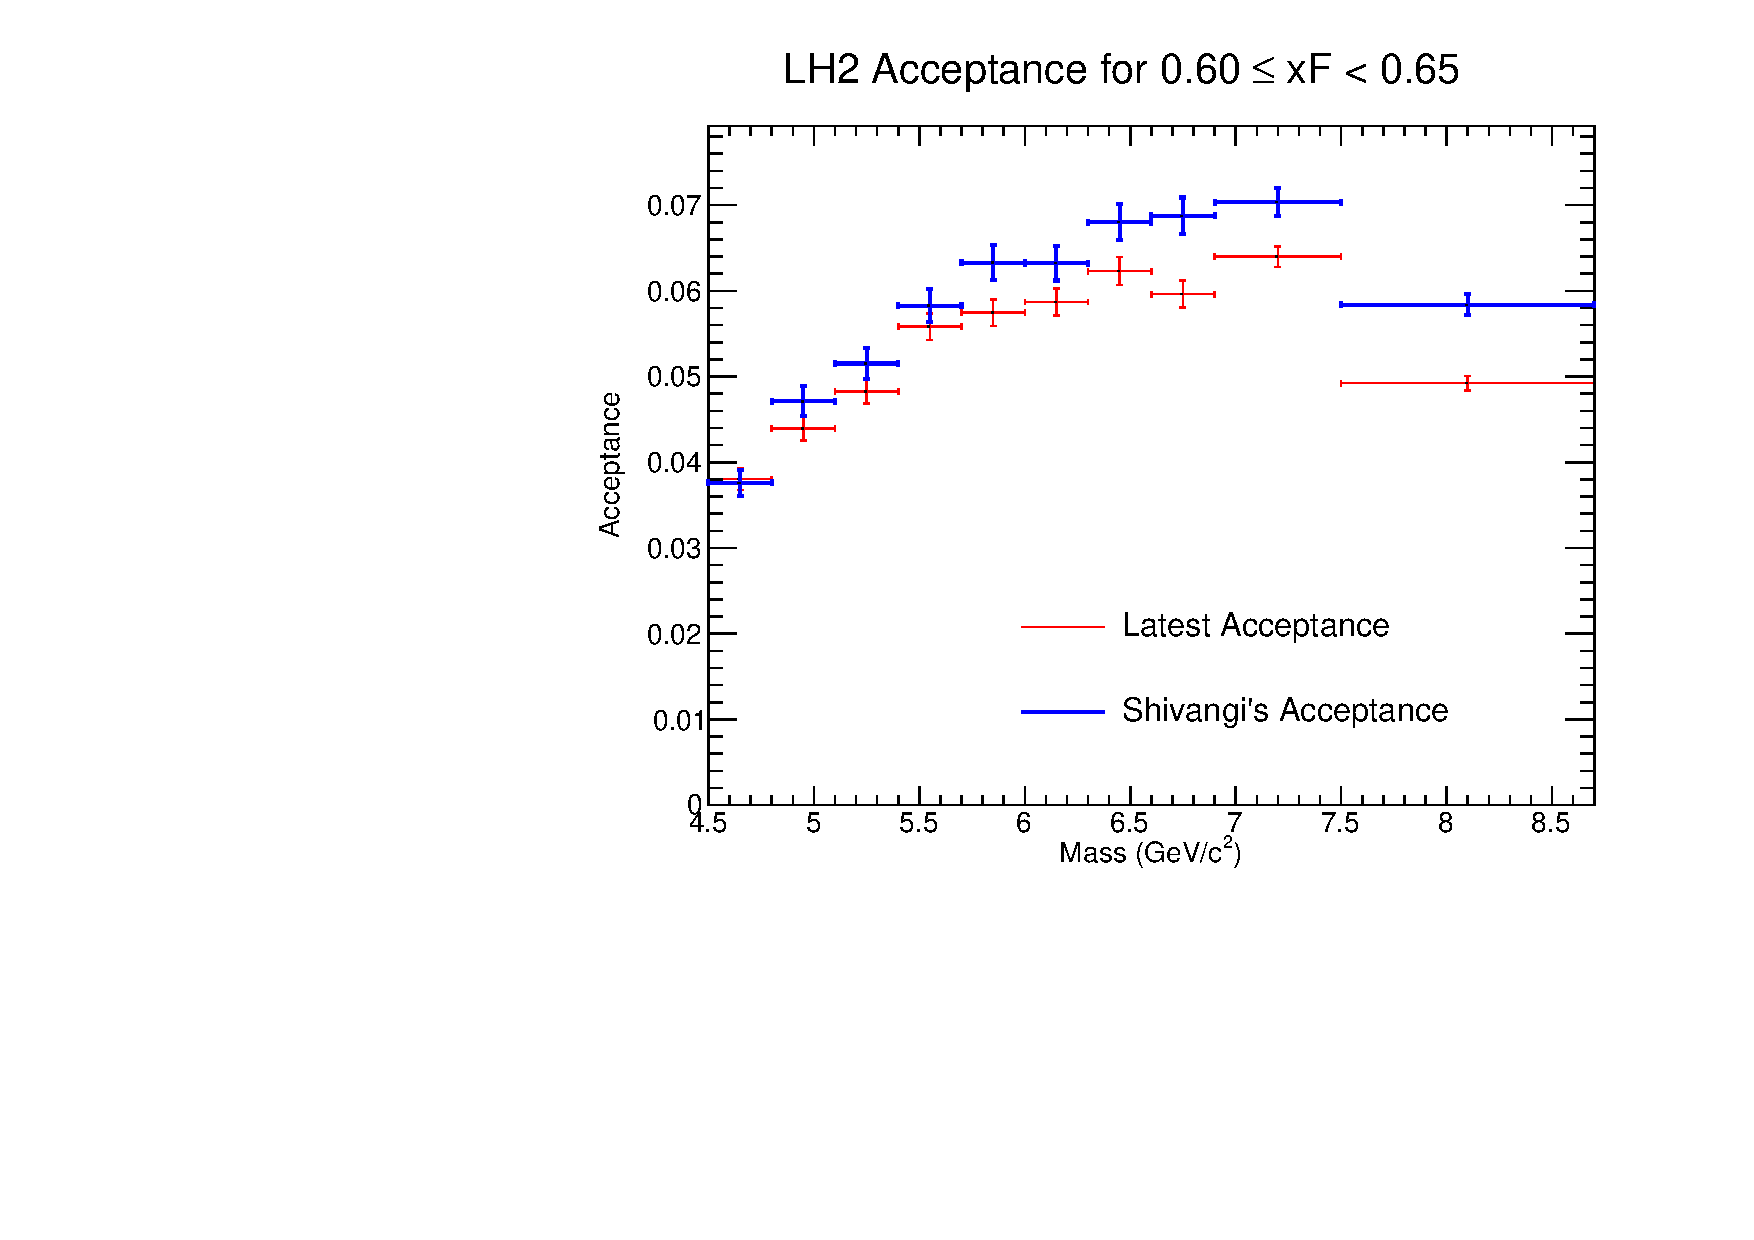
\includegraphics[width=\linewidth]{LH2_acceptance_xF_bin_12.pdf}
       \caption{Acceptance for LH2}
    \end{subfigure}
    \hfill
    \begin{subfigure}[b]{0.48\textwidth}
       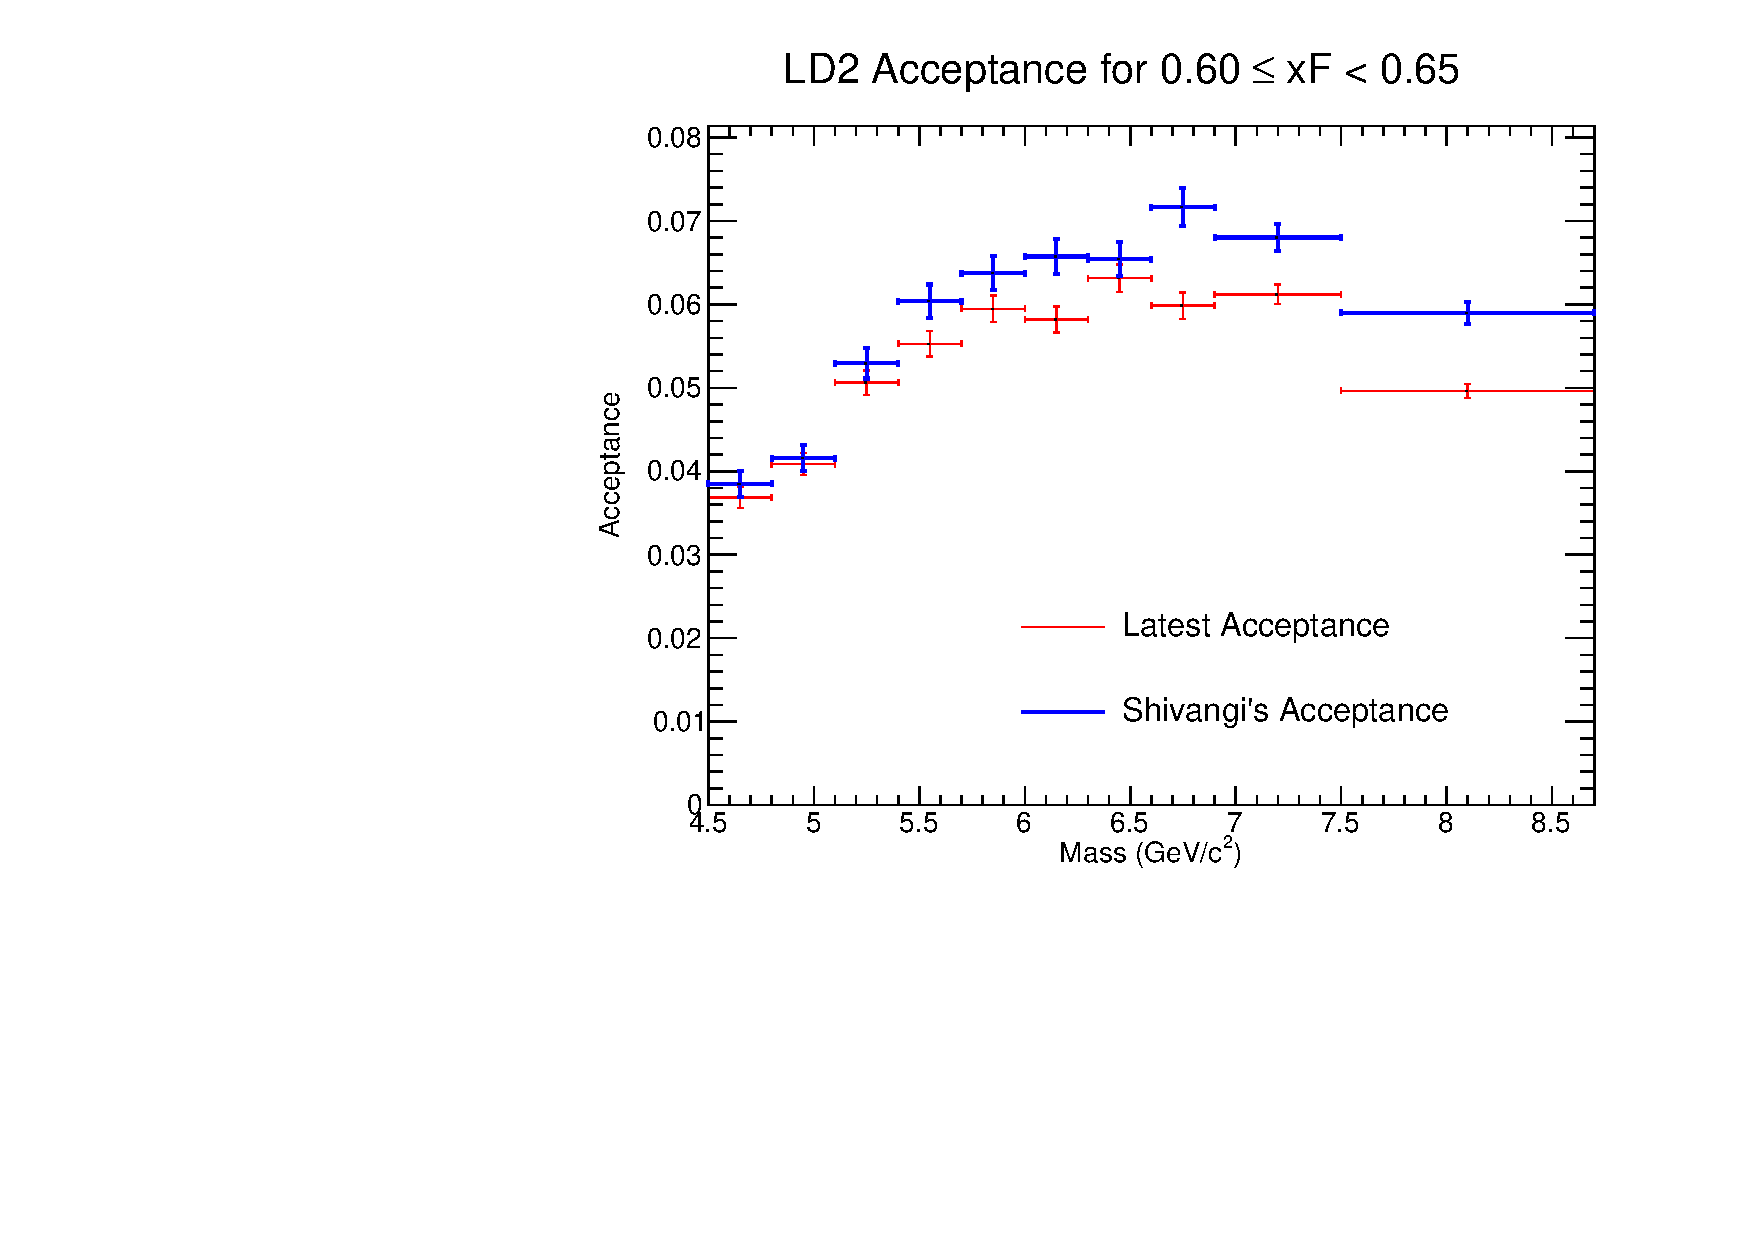
\includegraphics[width=\linewidth]{LD2_acceptance_xF_bin_12.pdf}
       \caption{Acceptance for LD2}
    \end{subfigure}

    \begin{subfigure}[b]{0.48\textwidth}
       \includegraphics[width=\linewidth]{Combined_acceptance_xF_bin_12.pdf}
       \caption{Combined Acceptance}
    \end{subfigure}
    \hfill
    \begin{subfigure}[b]{0.48\textwidth}
       \includegraphics[width=\linewidth]{Acceptance_ratio_xF_bin_12.pdf}
       \caption{Acceptance Ratio (LH2/LD2)}
    \end{subfigure}
    \caption{Acceptance plots for $0.60 \le x_F < 0.65$.}
\end{figure}

\begin{figure}[H]
    \centering
    \begin{subfigure}[b]{0.48\textwidth}
       \includegraphics[width=\linewidth]{LH2_acceptance_xF_bin_13.pdf}
       \caption{Acceptance for LH2}
    \end{subfigure}
    \hfill
    \begin{subfigure}[b]{0.48\textwidth}
       \includegraphics[width=\linewidth]{LD2_acceptance_xF_bin_13.pdf}
       \caption{Acceptance for LD2}
    \end{subfigure}

    \begin{subfigure}[b]{0.48\textwidth}
       \includegraphics[width=\linewidth]{Combined_acceptance_xF_bin_13.pdf}
       \caption{Combined Acceptance}
    \end{subfigure}
    \hfill
    \begin{subfigure}[b]{0.48\textwidth}
       \includegraphics[width=\linewidth]{Acceptance_ratio_xF_bin_13.pdf}
       \caption{Acceptance Ratio (LH2/LD2)}
    \end{subfigure}
    \caption{Acceptance plots for $0.65 \le x_F < 0.70$.}
\end{figure}

\begin{figure}[H]
    \centering
    \begin{subfigure}[b]{0.48\textwidth}
       \includegraphics[width=\linewidth]{LH2_acceptance_xF_bin_14.pdf}
       \caption{Acceptance for LH2}
    \end{subfigure}
    \hfill
    \begin{subfigure}[b]{0.48\textwidth}
       \includegraphics[width=\linewidth]{LD2_acceptance_xF_bin_14.pdf}
       \caption{Acceptance for LD2}
    \end{subfigure}

    \begin{subfigure}[b]{0.48\textwidth}
       \includegraphics[width=\linewidth]{Combined_acceptance_xF_bin_14.pdf}
       \caption{Combined Acceptance}
    \end{subfigure}
    \hfill
    \begin{subfigure}[b]{0.48\textwidth}
       \includegraphics[width=\linewidth]{Acceptance_ratio_xF_bin_14.pdf}
       \caption{Acceptance Ratio (LH2/LD2)}
    \end{subfigure}
    \caption{Acceptance plots for $0.70 \le x_F < 0.75$.}
\end{figure}

\begin{figure}[H]
    \centering
    \begin{subfigure}[b]{0.48\textwidth}
       \includegraphics[width=\linewidth]{LH2_acceptance_xF_bin_15.pdf}
       \caption{Acceptance for LH2}
    \end{subfigure}
    \hfill
    \begin{subfigure}[b]{0.48\textwidth}
       \includegraphics[width=\linewidth]{LD2_acceptance_xF_bin_15.pdf}
       \caption{Acceptance for LD2}
    \end{subfigure}

    \begin{subfigure}[b]{0.48\textwidth}
       \includegraphics[width=\linewidth]{Combined_acceptance_xF_bin_15.pdf}
       \caption{Combined Acceptance}
    \end{subfigure}
    \hfill
    \begin{subfigure}[b]{0.48\textwidth}
       \includegraphics[width=\linewidth]{Acceptance_ratio_xF_bin_15.pdf}
       \caption{Acceptance Ratio (LH2/LD2)}
    \end{subfigure}
    \caption{Acceptance plots for $0.75 \le x_F < 0.80$.}
\end{figure}


\end{document}
